\documentclass{article}
\usepackage[framed,numbered,autolinebreaks,useliterate]{mcode}
\usepackage[utf8]{inputenc}
\usepackage[T1]{fontenc}
\usepackage[polish]{babel}
\usepackage{lmodern}
\selectlanguage{polish}
\usepackage{float}
\usepackage{hyperref}
\usepackage{color}
\usepackage{graphicx} 
\usepackage{float}
\usepackage{enumerate}
\usepackage{framed}
\hypersetup{
    colorlinks,
    citecolor=black,
    filecolor=black,
    linkcolor=black,
    urlcolor=black
}
\author{Bartosz Rajkowski}
\title{Projekt I STP\\zadanie 1.9}
\date{30 kwietnia 2017}

\begin{document}
\maketitle
\newpage
\tableofcontents
\newpage

\section*{Dane}
$$
G(s)=\frac{0,5s^2+3,5s+5,625}{s^3+8s^2-36s-288}
$$
\section{Zadanie 1}
\subsection{Treść}

Wyznaczyć transmitancję dyskretną $G(z)$, stosując ekstrapolator zerowego rzędu i przyjmując okres próbkowania $T_p=0,1s$. Określić zera i bieguny obydwu transmitancji. Odpowiedzieć na pytanie, czy obiekt jest stabilny.

\subsection{Program}
\lstinputlisting[caption={zad1.m}, label={lst:zad1}]{../zad1.m}
\subsection{Wyniki}
\subsubsection{Transmitancja dyskretna}
$$
G(z)=\frac{0.05183 z^2 - 0.07375 z + 0.0259}{z^3 - 2.82 z^2 + 2.065 z - 0.4493}
$$
\subsubsection[Bieguny i zera]{Bieguny i zera transmitancji ciągłej i dyskretnej}
\begin{enumerate}
\item Transmitancja ciągła
\begin{itemize}
\item Bieguny: \verb+6 -8 -6+
\item Zera: \verb+-4.5 -2.5+
\end{itemize}

\item Transmitancja dyskretna
\begin{itemize}
\item Bieguny: \verb+1.8221 0.5488 0.4493+
\item Zera: \verb+ -4.5 -2.5+
\end{itemize}
\end{enumerate}
\begin{figure}[t]
\centering
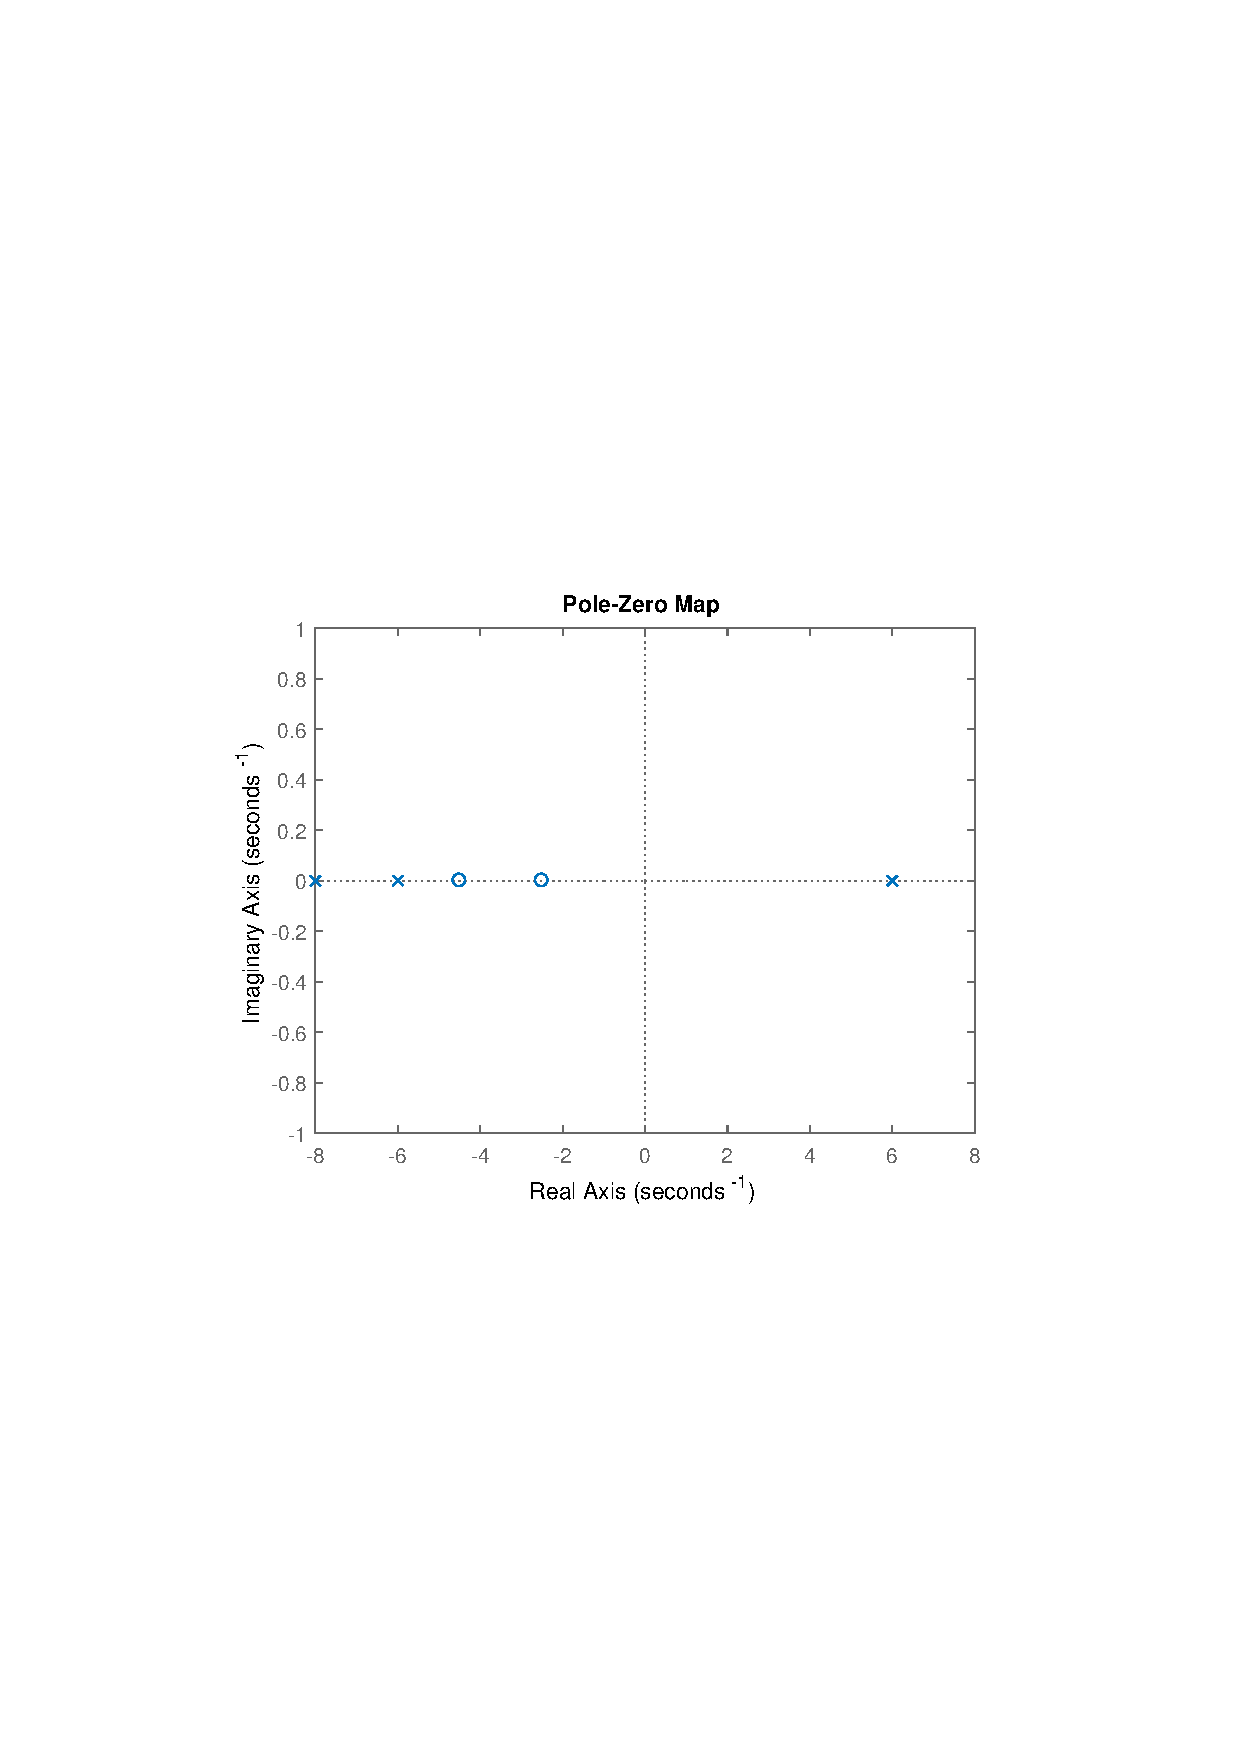
\includegraphics[clip, trim=3cm 9cm 3cm 9.5cm, width=9.5cm]{../rys/zad1_rys1.pdf}
\caption{Zera i bieguny transmitancji ciągłej}
\label{fig:rys 1}
\end{figure}

\begin{figure}[H]
\centering
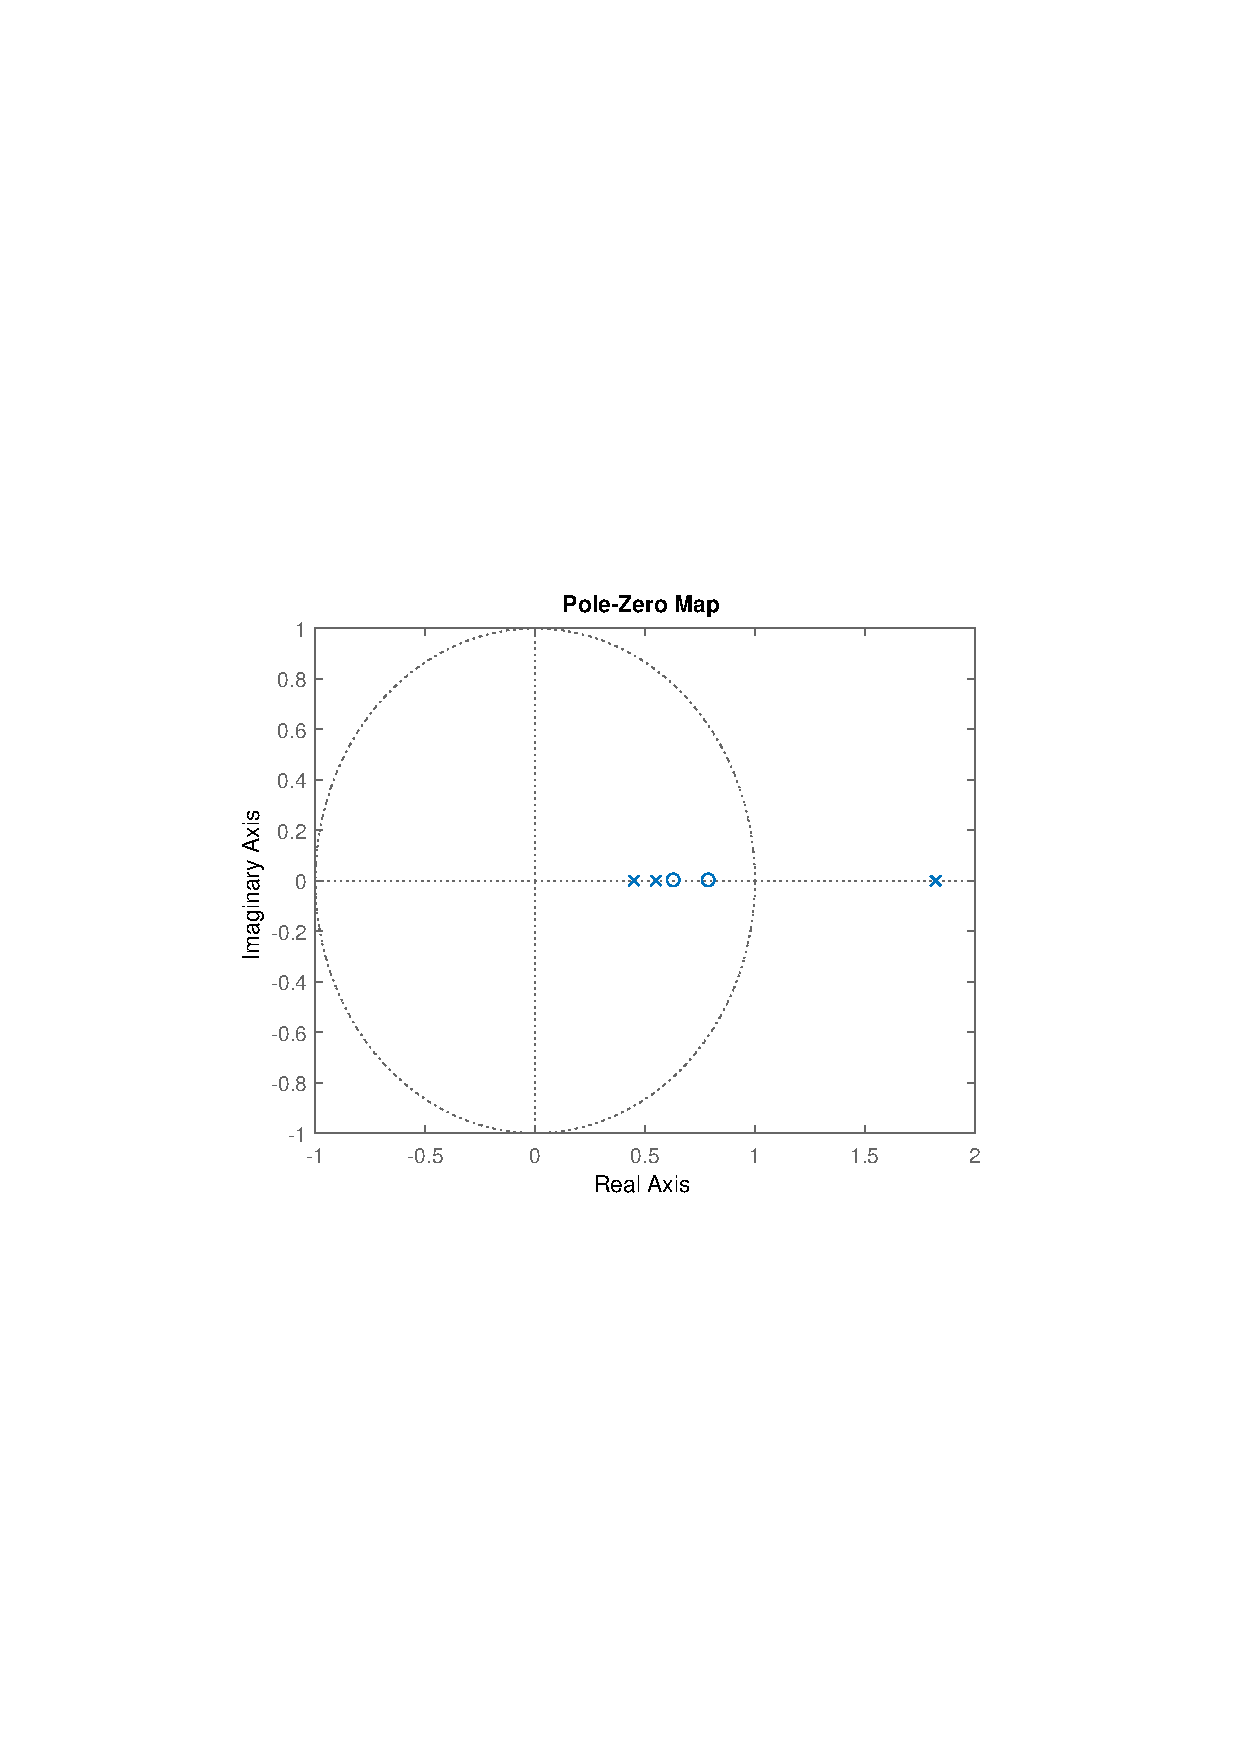
\includegraphics[clip, trim=3cm 9cm 3cm 9.5cm, width=9.5cm]{../rys/zad1_rys2.pdf}
\caption{Zera i bieguny transmitancji dyskretnej}
\label{fig:rys 2}
\end{figure}

\subsubsection{Wnioski}
Układ dyskretny jest stabilny tylko wtedy, gdy wszystkie jego bieguny leżą w~kole o promieniu 1 i środku w początku układu współrzędnych. Jak widać na~rysunku jeden z biegunów leży poza kołem, zatem układ nie jest stabilny.
\section{Zadanie 2}
\subsection{Treść}
Znaleźć reprezentację modelu dyskretnego w przestrzeni stanów stosując dwa warianty
metody bezpośredniej wyznaczania równań stanu na podstawie transmitancji, a następnie
narysować schematy otrzymanych modeli.
\subsection{Sposób rozwiązania}
Transmitancję dyskretną można obliczyć ze wzoru:
$$
G(z)=C(zI-A)^{-1}B+D
$$
W Matlabie służy do tego polecenie \verb+tf2ss+.
Wariant drugi możemy wyznaczyć z pierwszego.
Wtedy
$$
A2=A^T, B2=C^T, C2=B^T, D2=D
$$
\subsection{Program}
\lstinputlisting[caption={zad2.m}, label={lst:zad2}]{../zad2.m}
\vbox{
\subsection{Wyniki}
\subsubsection{Wariant pierwszy}
\begin{tabular}{l}
$
A=\left[\begin{array}{ccc} 2.82 & -2.065 & 0.4493\\ 1 & 0 & 0\\ 0 & 1 & 0 \end{array}\right]
$\\\\
$
B=\left[\begin{array}{c} 1\\ 0\\ 0 \end{array}\right],
C=\left[\begin{array}{ccc} 0.05183 & -0.07375 & 0.0259 \end{array}\right],
D=0
$
\end{tabular}
\begin{figure}[H]
                                                     
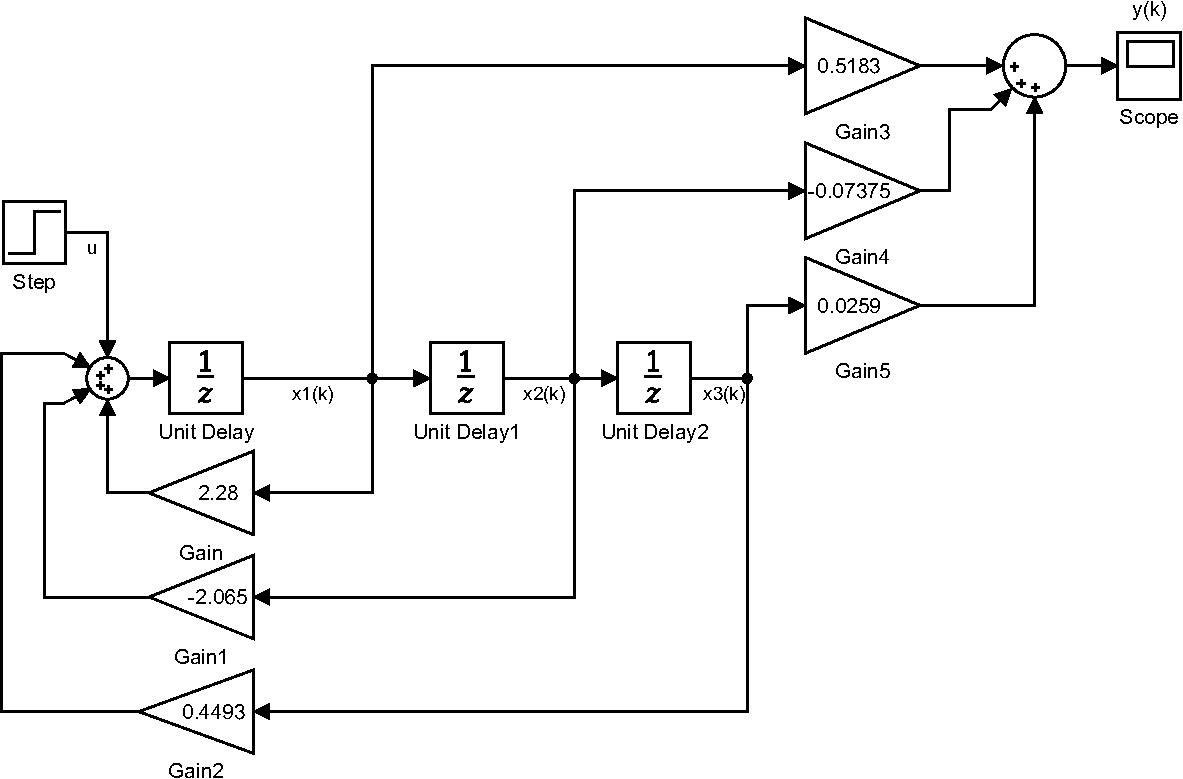
\includegraphics[ width=1.00\textwidth]{../rys/zad2_wariant1.pdf}
\caption{Diagram wariant 1}
\label{fig:diag1}
\end{figure}
}
\vbox{
\subsubsection{Wariant drugi}
\begin{tabular}{l}
$
A=\left[\begin{array}{ccc} 2.82 & 1 & 0\\ -2.065 & 0 & 1\\ 0.4493 & 0 & 0 \end{array}\right]
$\\\\
$
B=\left[\begin{array}{c} 0.05183\\ -0.07375\\ 0.0259 \end{array}\right],
C=\left[\begin{array}{ccc} 1 & 0 & 0 \end{array}\right],
D=0
$
\end{tabular}

\begin{figure}[H]
                                                       
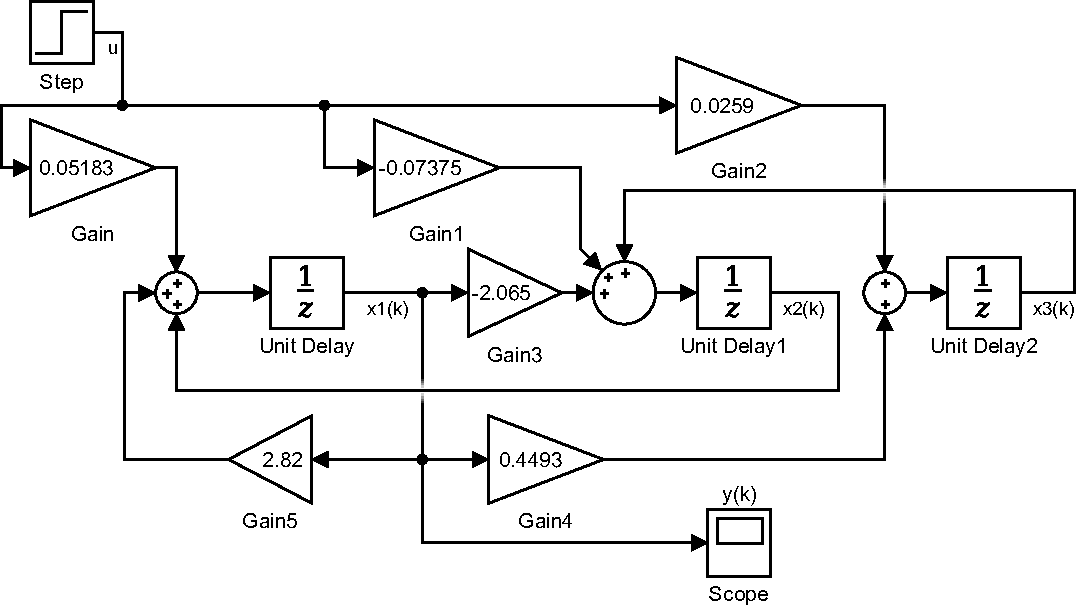
\includegraphics[ width=1.00\textwidth]{../rys/zad2_wariant2.pdf}
\caption{Diagram wariant 2}
\label{fig:diag2}
\end{figure}
}
\newpage
\section{Zadanie 3}
\subsection{Treść}
Wyznaczyć wektor sprzężeń zwrotnych K w taki sposób, aby układ zamknięty miał:
\begin{enumerate}[a)]
\item takie same bieguny, tzn. \verb+z1=z2=z3+,
\item biegun dominujący a dwa pozostałe bieguny dobrane tak, aby nie wpływały na działanie układu regulacji.
\end{enumerate}
\subsection{Układ zamknięty}
W układzie zamkniętym ze sprzężeniem od stanu sygnał \verb+u(k)+ wyraża się wzorem:
$$
u(k)=-Kx(k)=-[k_1 k_2 k_3]\left[\begin{array}{c} x_1\\ x_2\\ x_3 \end{array}\right]
$$
Zatem:
$$
x(k+1)=Ax(k)-BKx(k)=(A-BK)x(k)
$$
Odpowiednie dopasowanie wektora K pozwala na zadane ustalenie położenia biegunów.
\subsection{Program}
\vbox{
\lstinputlisting[caption={zad3a.m}, label={lst:zad3a}]{../zad3a.m}
}
\vbox{
\lstinputlisting[caption={zad3b.m}, label={lst:zad3b}]{../zad3b.m}
}
\vbox{
\lstinputlisting[caption={zad3max.m}, label={lst:zad3max}]{../zad3max.m}
}
\subsection{Zadanie a)}
\subsubsection{Wykresy}
\begin{figure}[H]
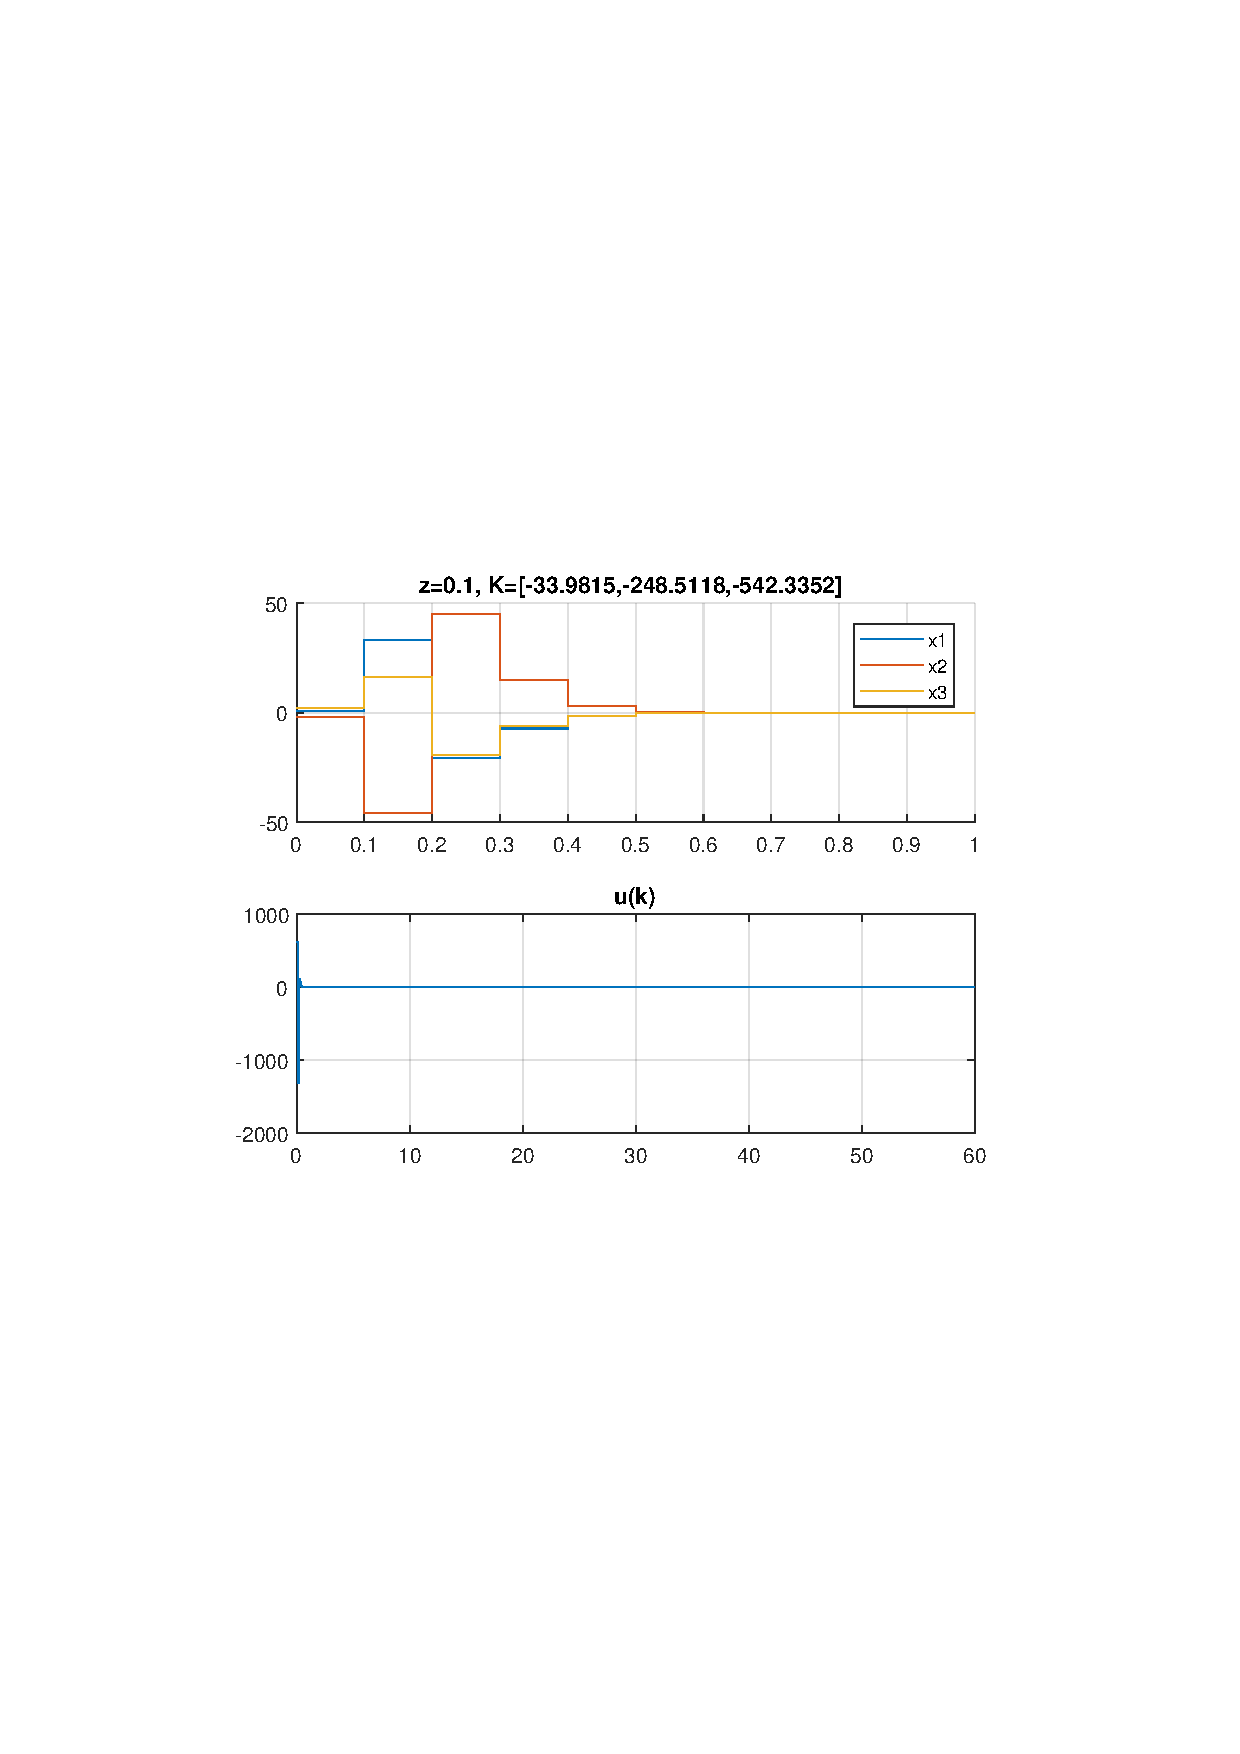
\includegraphics[clip, trim=0.5cm 9.5cm 0.5cm 9.5cm, width=1.00\textwidth]{../rys/zad3_rys1.pdf}
\label{fig:rys3.1.1}

\end{figure}
\vbox{
\begin{figure}[H]
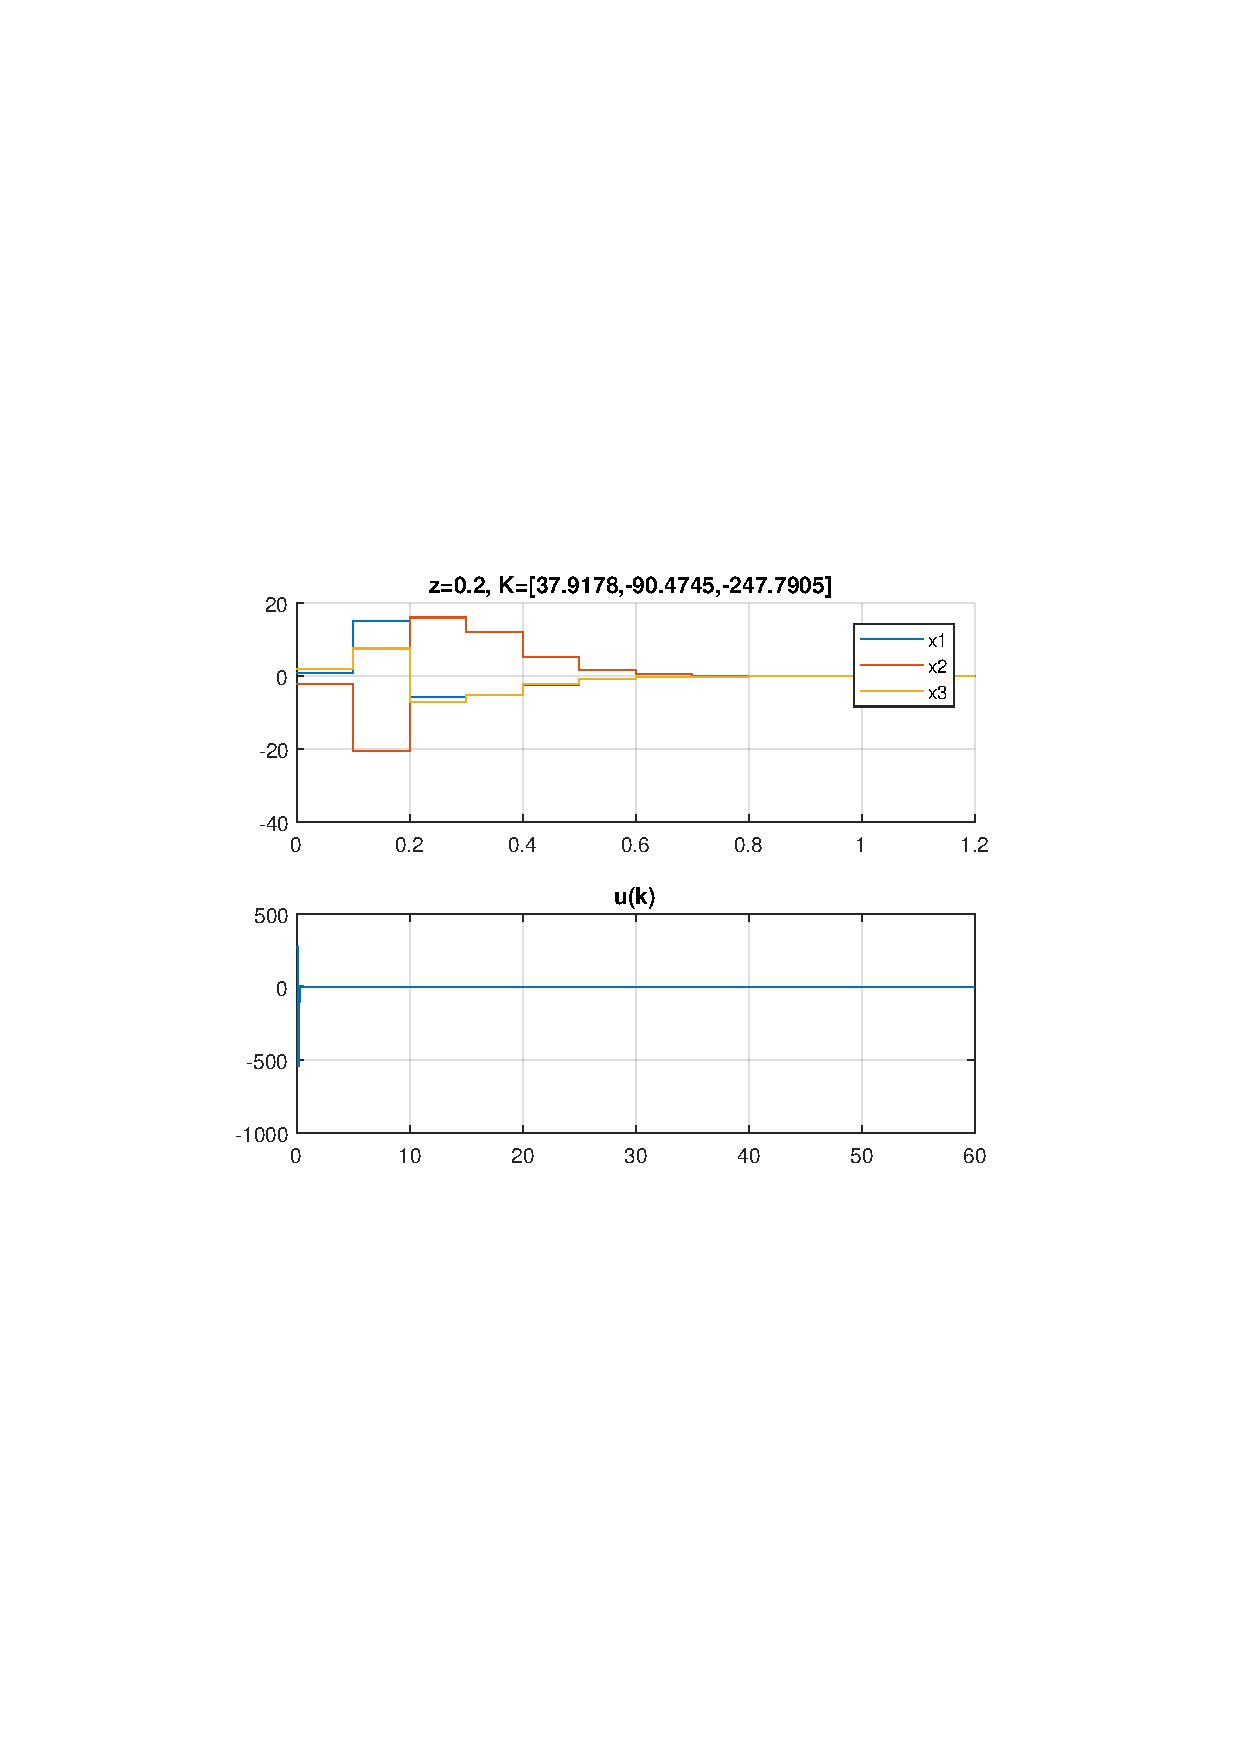
\includegraphics[clip, trim=0.5cm 9.5cm 0.5cm 9.5cm, width=1.00\textwidth]{../rys/zad3_rys2.pdf}
\label{fig:rys3.1.2}
\caption{1.2}
\end{figure}

\begin{figure}[H]
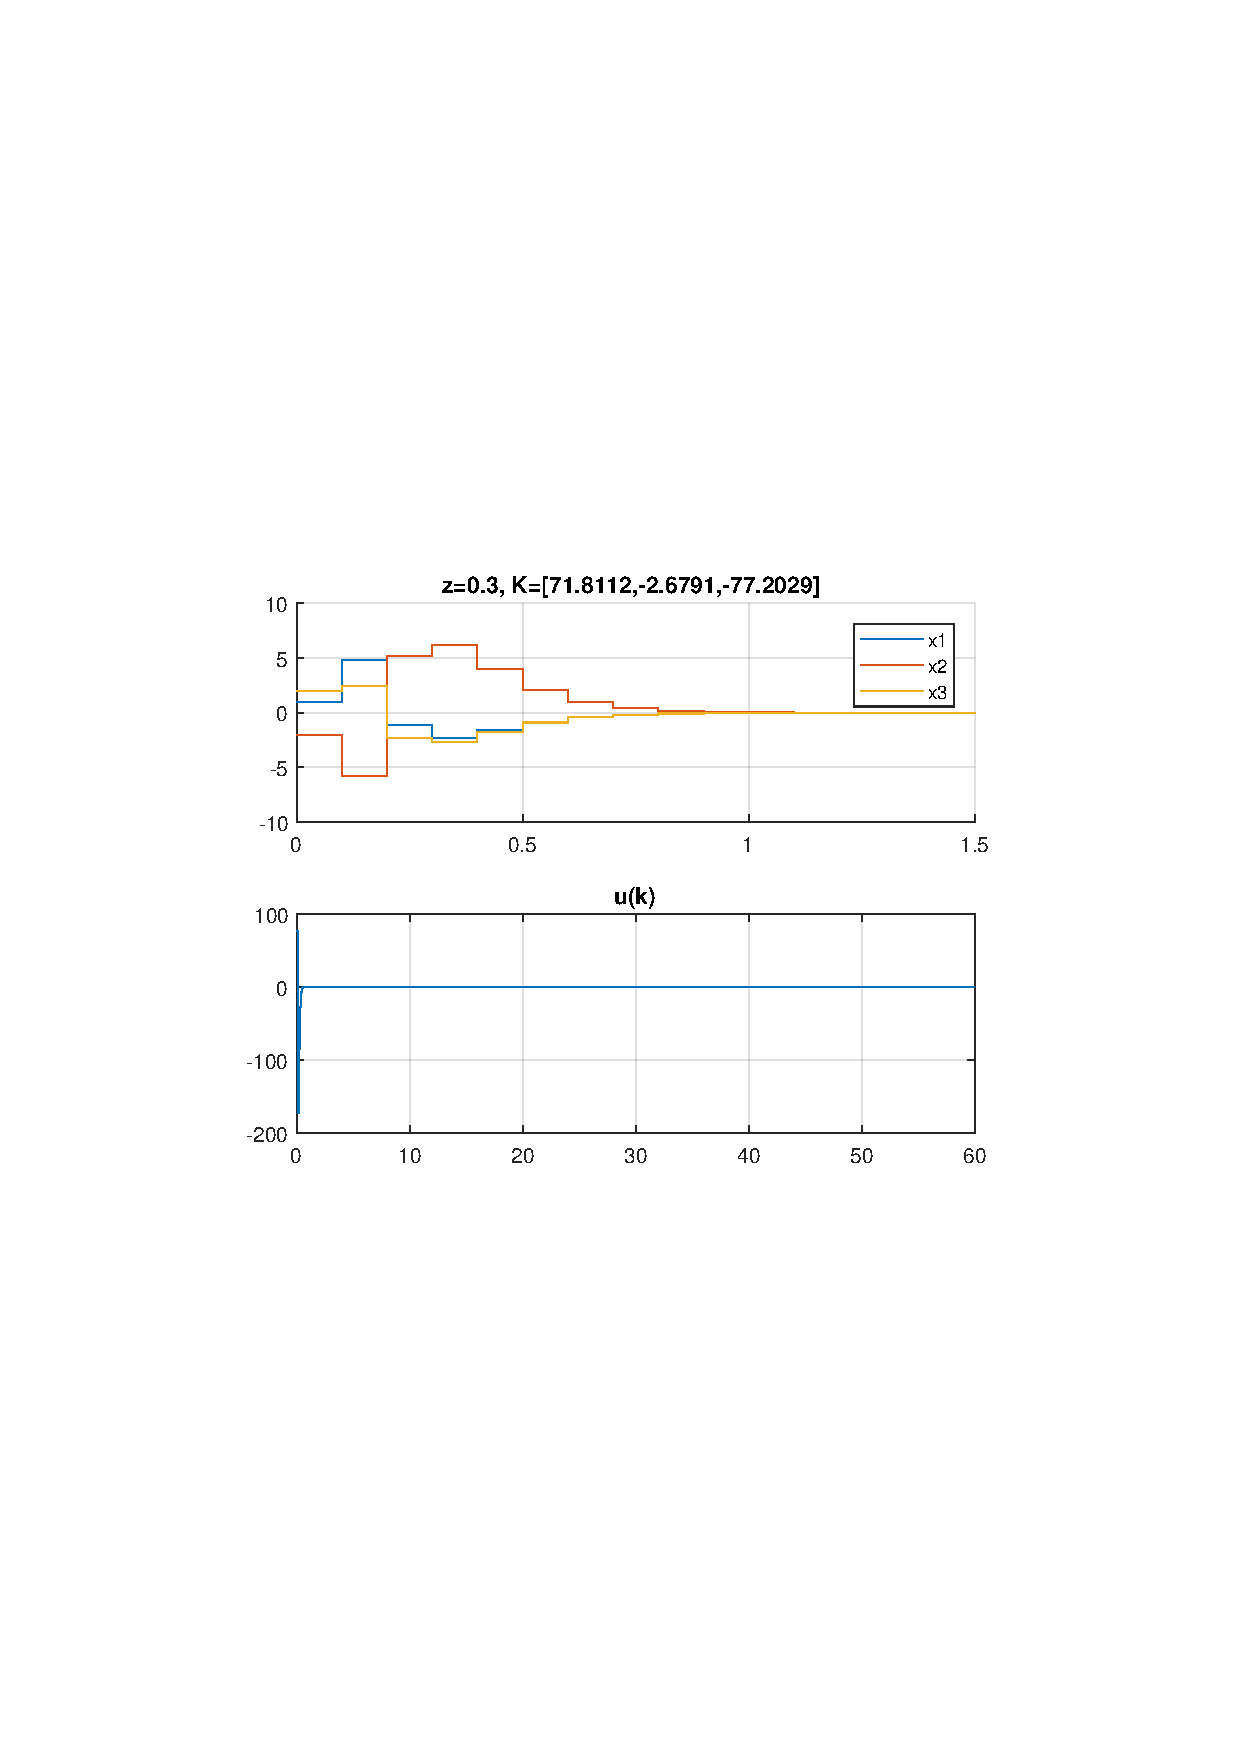
\includegraphics[clip, trim=0.5cm 9.5cm 0.5cm 9.5cm, width=1.00\textwidth]{../rys/zad3_rys3.pdf}
\label{fig:rys3.1.3}
\caption{1.3}
\end{figure}
}
\vbox{
\begin{figure}[H]
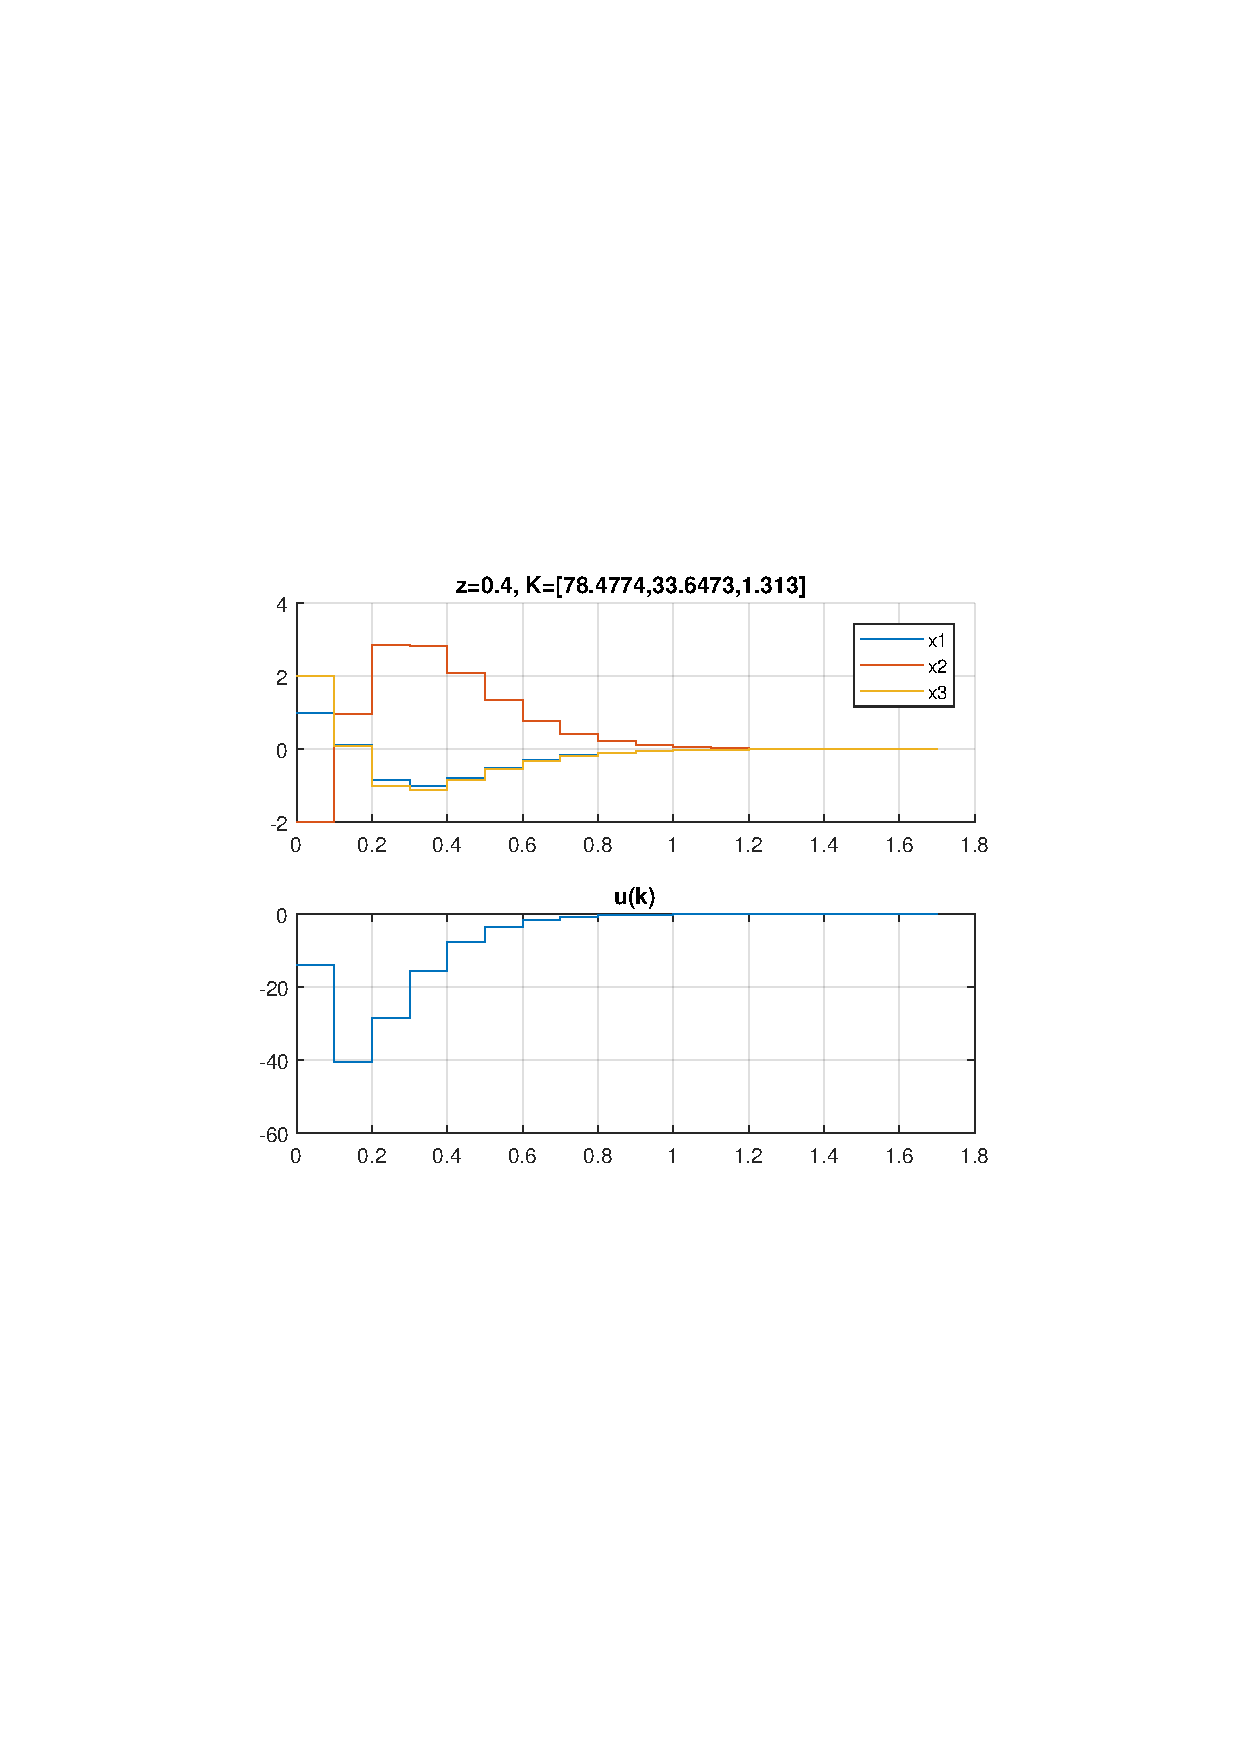
\includegraphics[clip, trim=0.5cm 9.5cm 0.5cm 9.5cm, width=1.00\textwidth]{../rys/zad3_rys4.pdf}
\label{fig:rys3.1.4}
\caption{1.4}
\end{figure}
\begin{figure}[H]
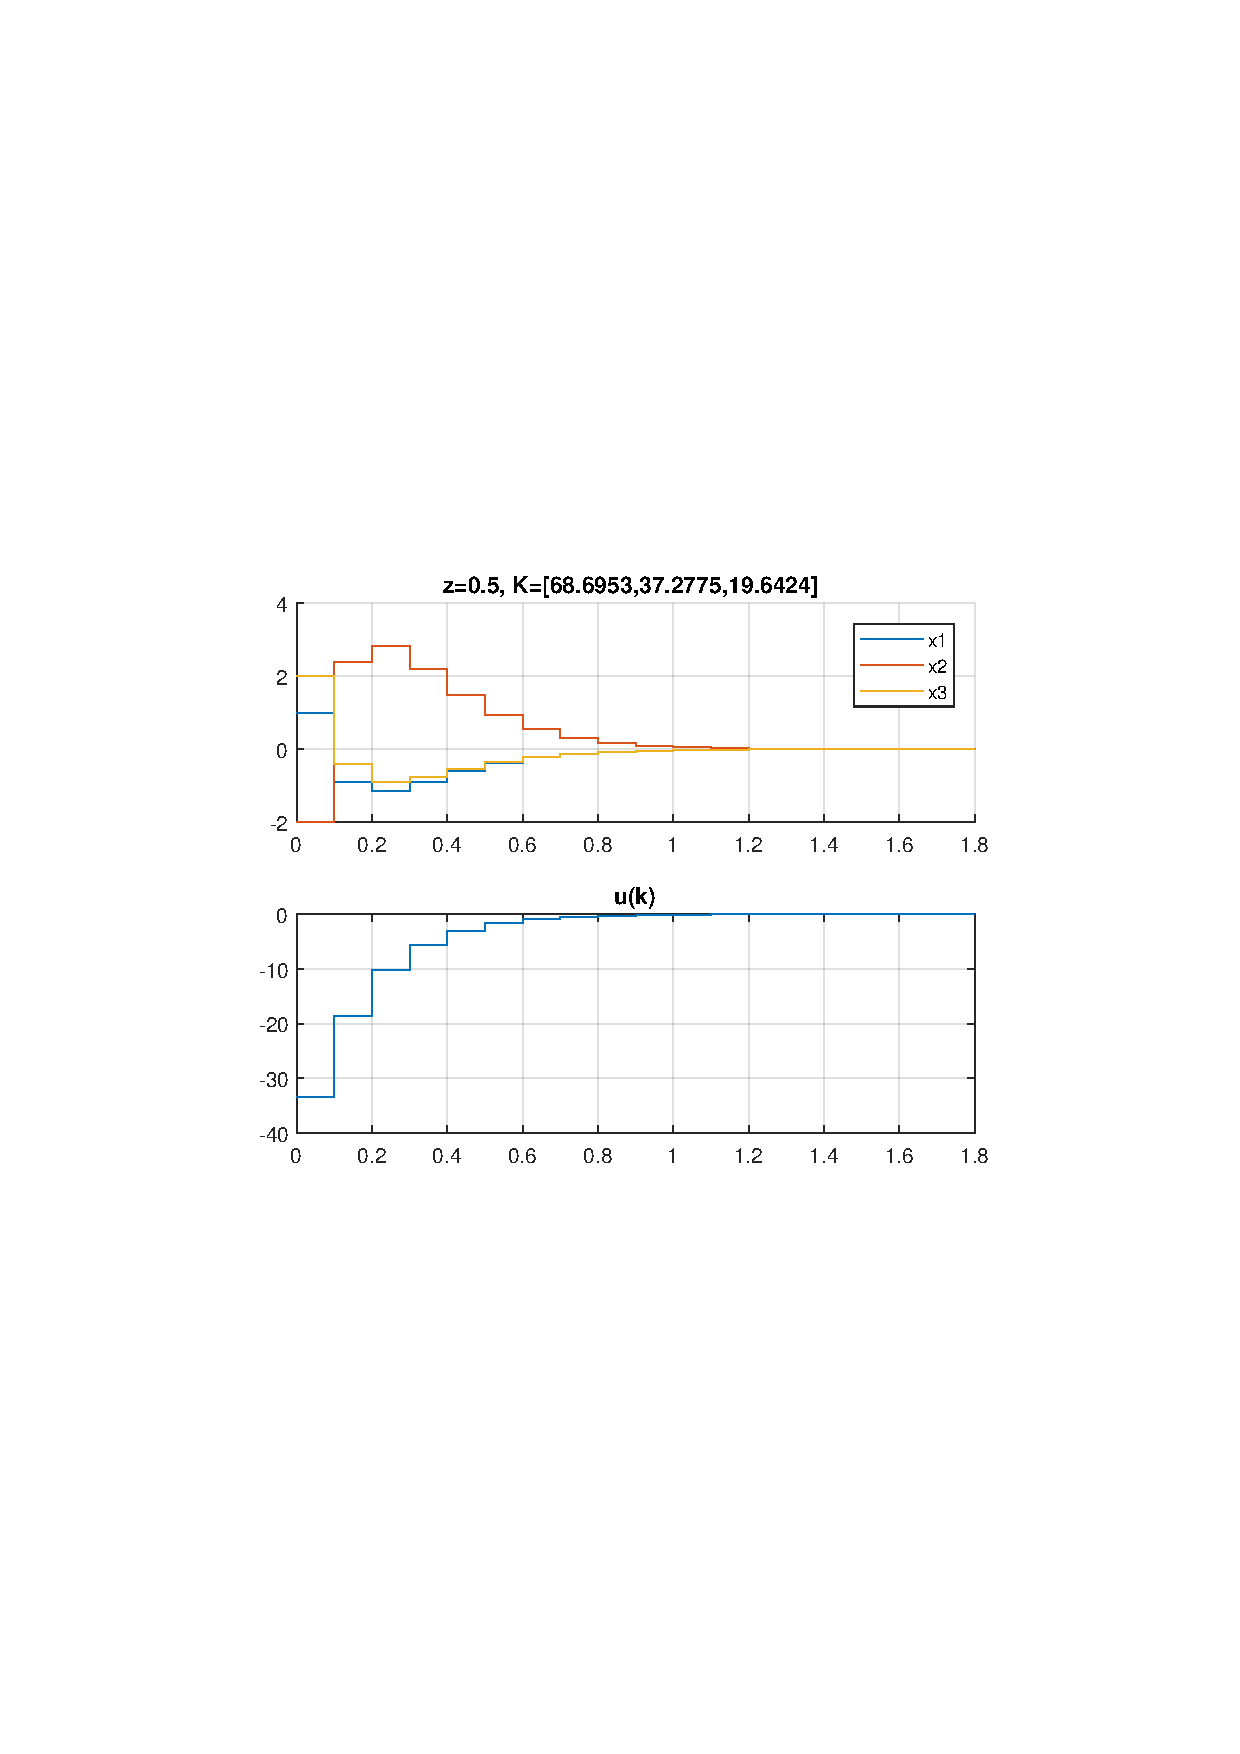
\includegraphics[clip, trim=0.5cm 9.5cm 0.5cm 9.5cm, width=1.00\textwidth]{../rys/zad3_rys5.pdf}
\label{fig:rys3.1.5}
\caption{1.5}
\end{figure}
}
\vbox{
\begin{figure}[H]
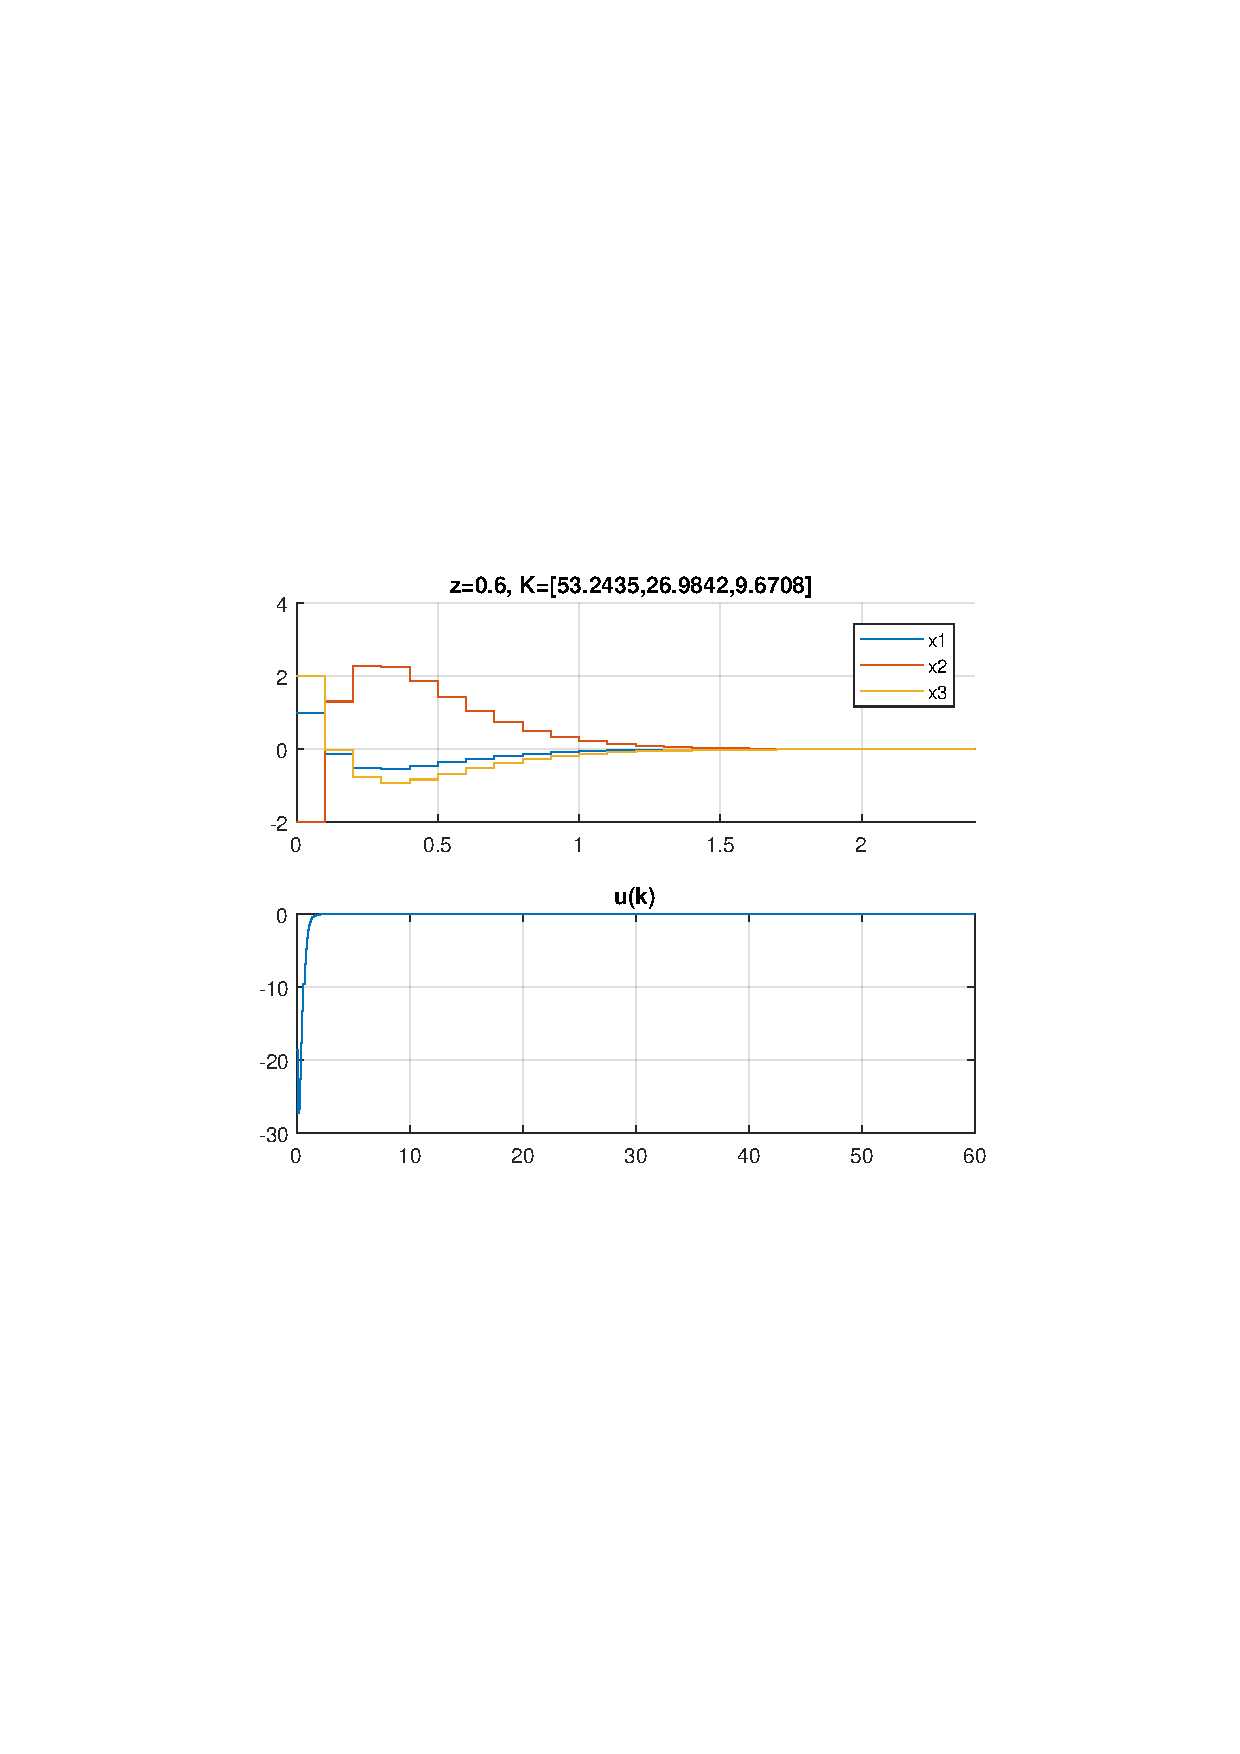
\includegraphics[clip, trim=0.5cm 9.5cm 0.5cm 9.5cm, width=1.00\textwidth]{../rys/zad3_rys6.pdf}
\label{fig:rys3.1.6}
\caption{1.6}
\end{figure}
\begin{figure}[H]
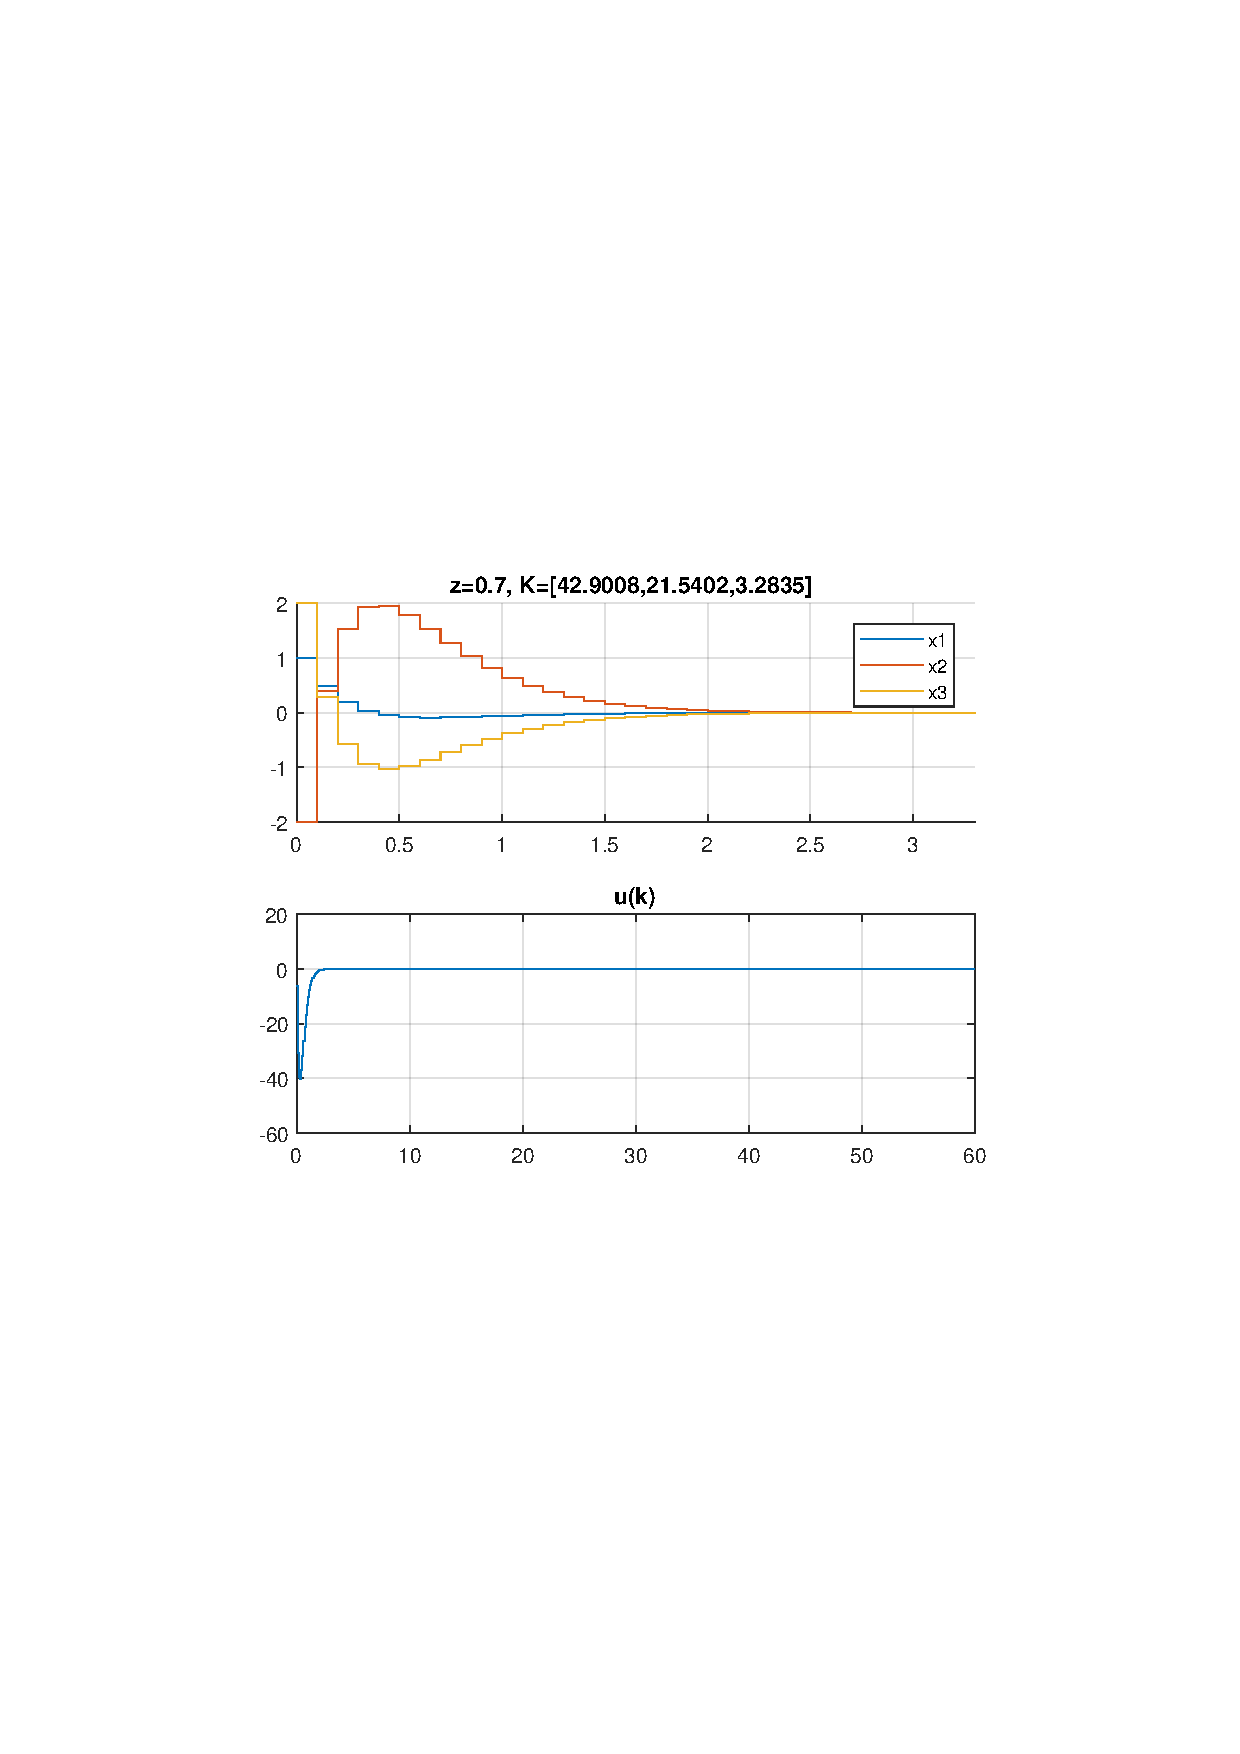
\includegraphics[clip, trim=0.5cm 9.5cm 0.5cm 9.5cm, width=1.00\textwidth]{../rys/zad3_rys7.pdf}
\label{fig:rys3.1.7}
\caption{1.7}
\end{figure}
}
\vbox{
\begin{figure}[H]
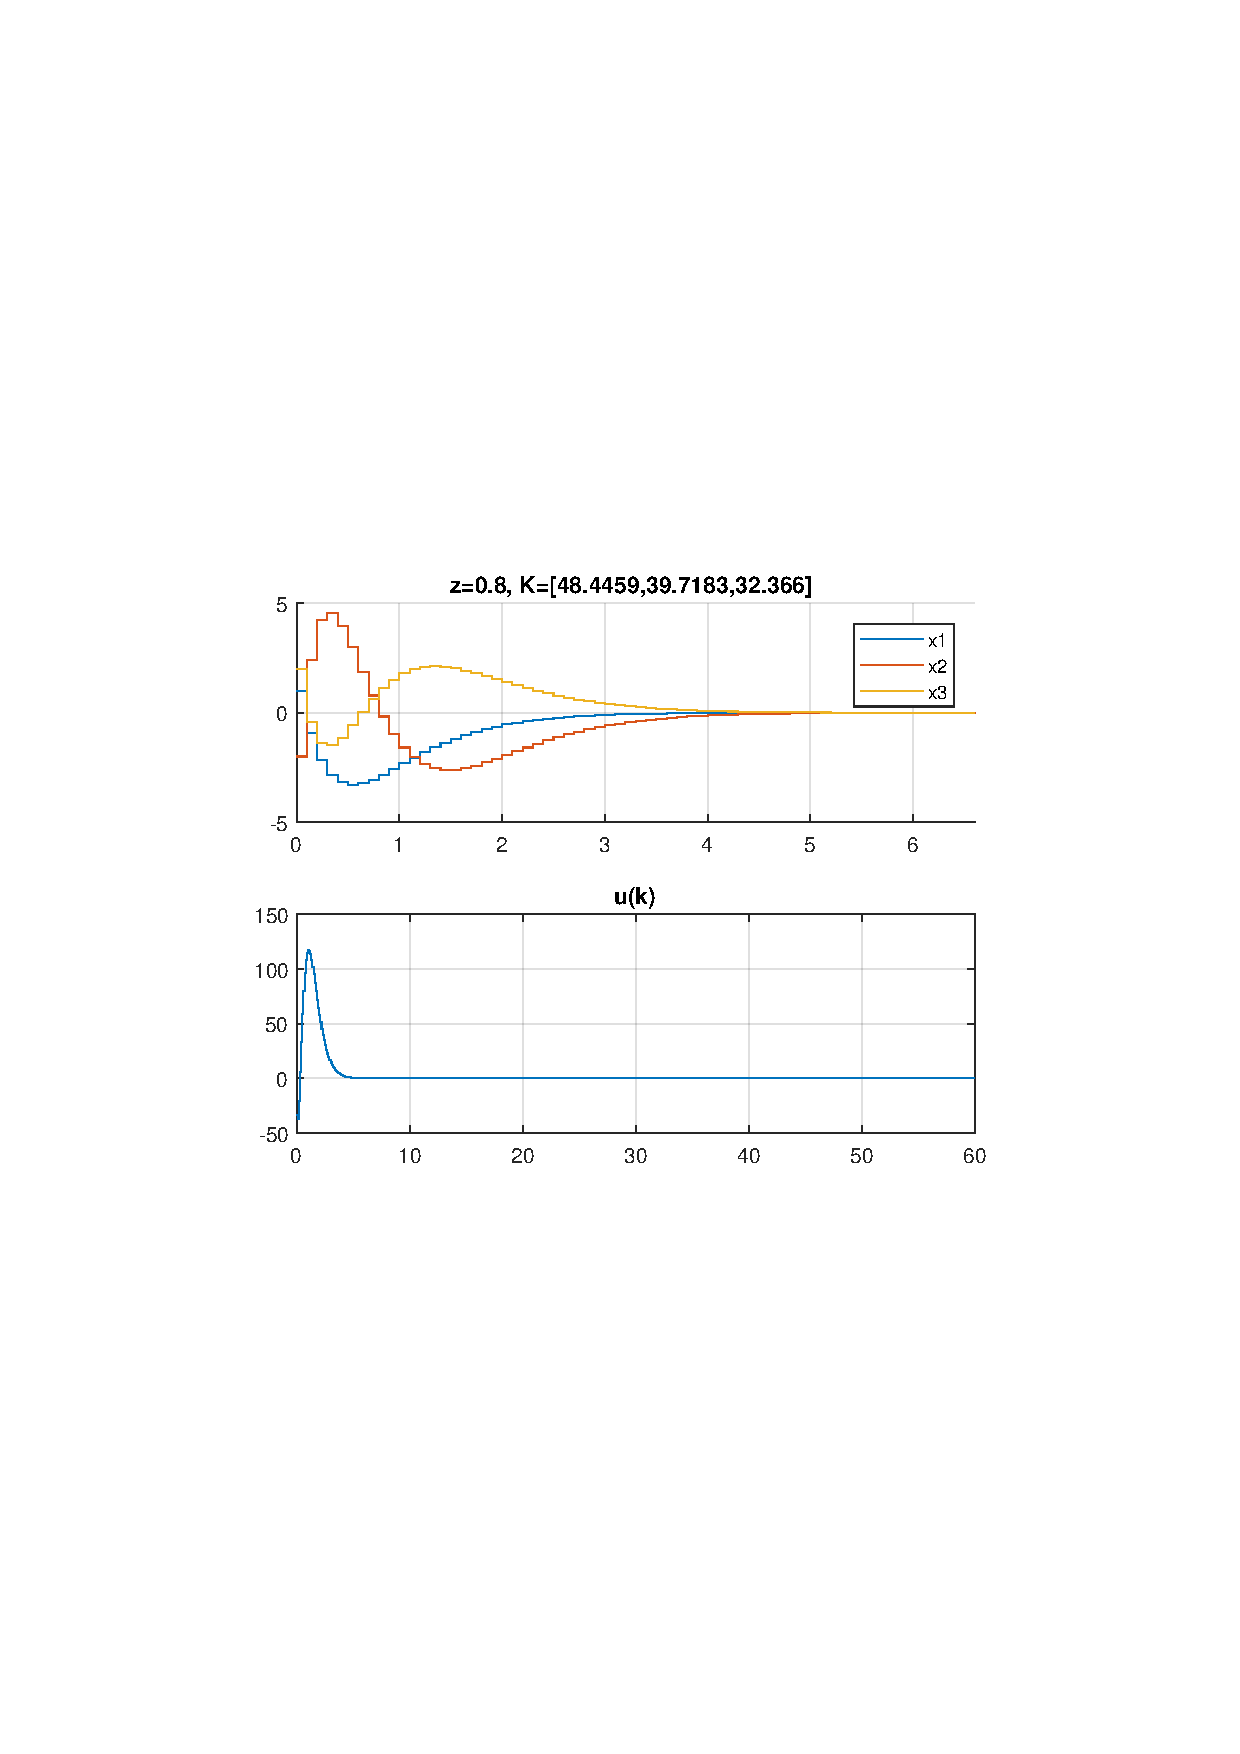
\includegraphics[clip, trim=0.5cm 9.5cm 0.5cm 9.5cm, width=1.00\textwidth]{../rys/zad3_rys8.pdf}
\label{fig:rys3.1.8}
\caption{1.8}
\end{figure}
\begin{figure}[H]
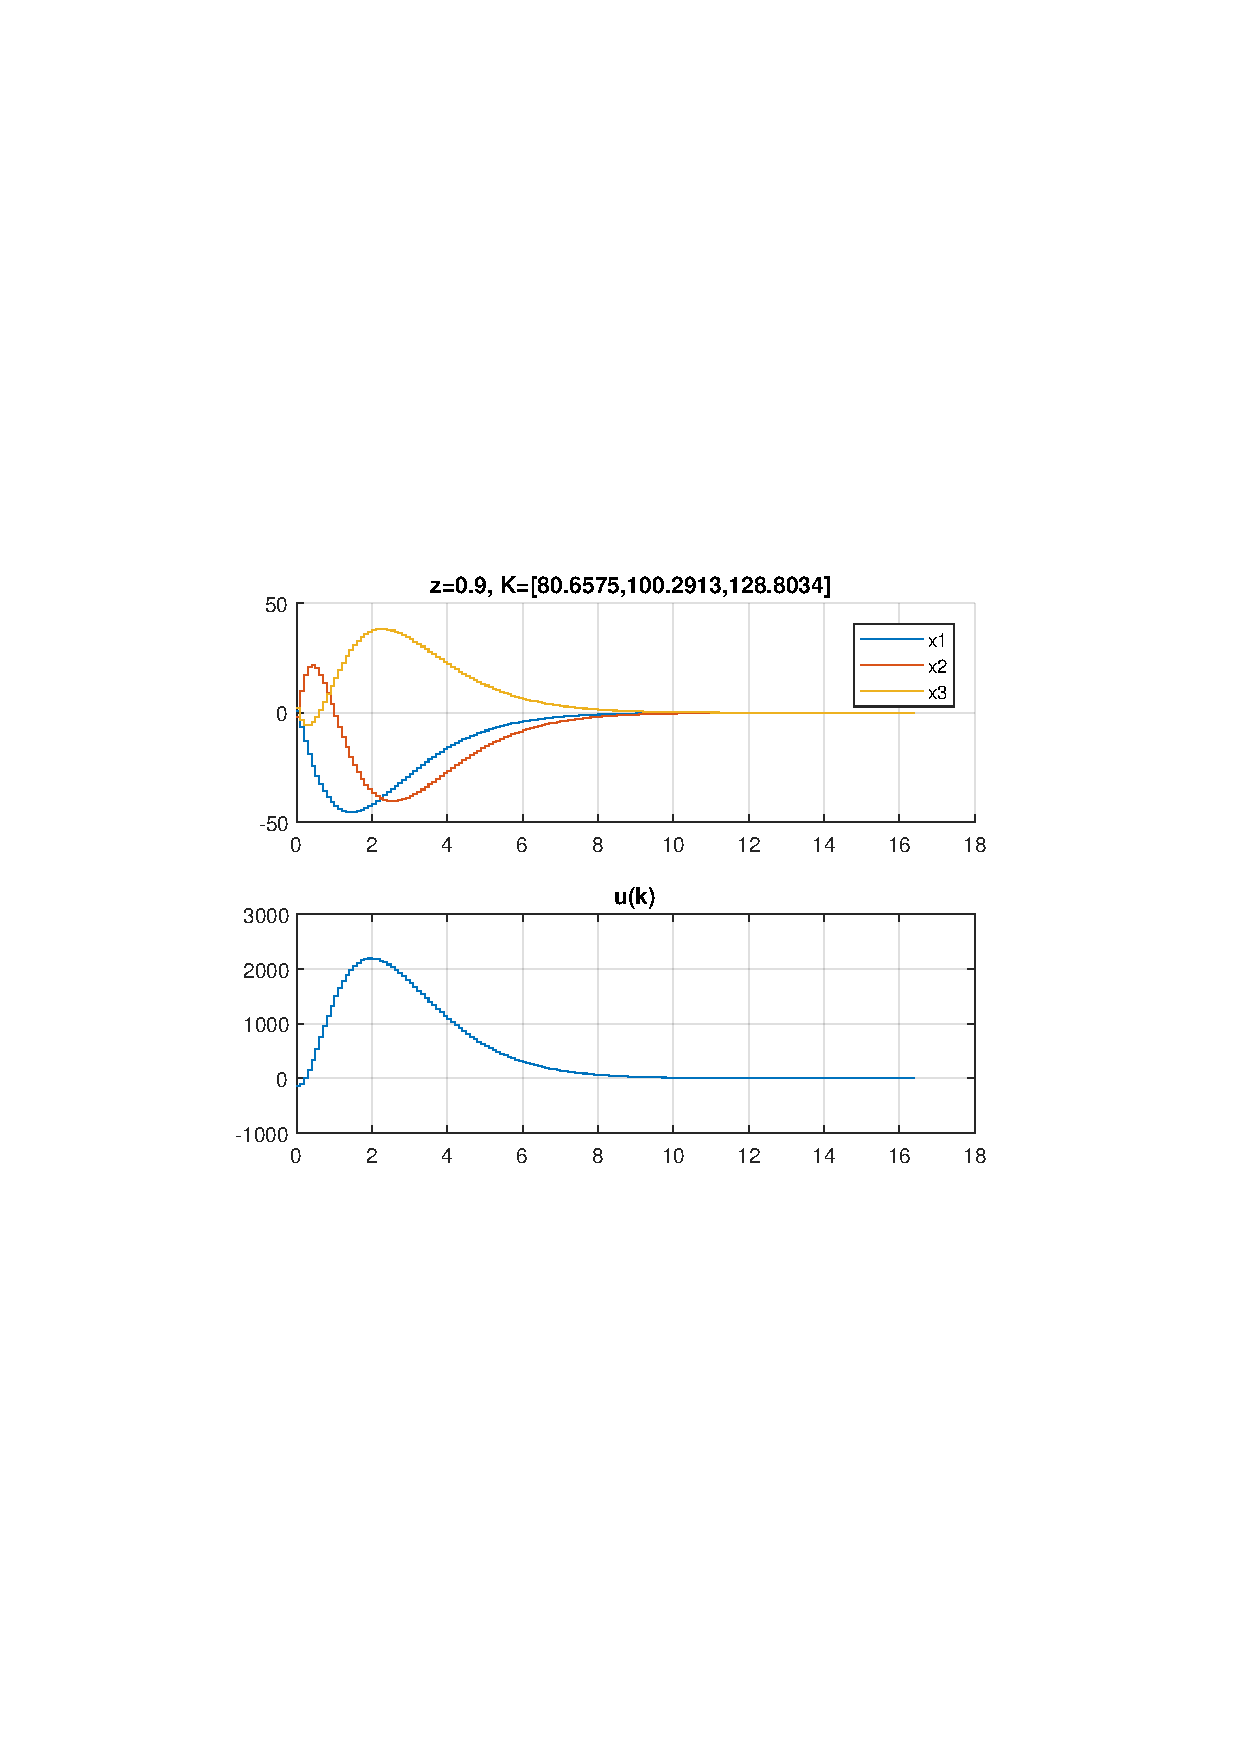
\includegraphics[clip, trim=0.5cm 9.5cm 0.5cm 9.5cm, width=1.00\textwidth]{../rys/zad3_rys9.pdf}
\label{fig:rys3.1.9}
\caption{1.9}
\end{figure}
}
\newpage
\subsubsection[Przyrost sterowania]{Zależność maksymalnego przyrostu sterowania od położenia biegunów}
Przeprowadziłem 19 eksperymentów dla $z \in\{0.05, 0.1, \ldots, 0.95\}$. Wynik na poniższym wykresie.
\begin{figure}[H]
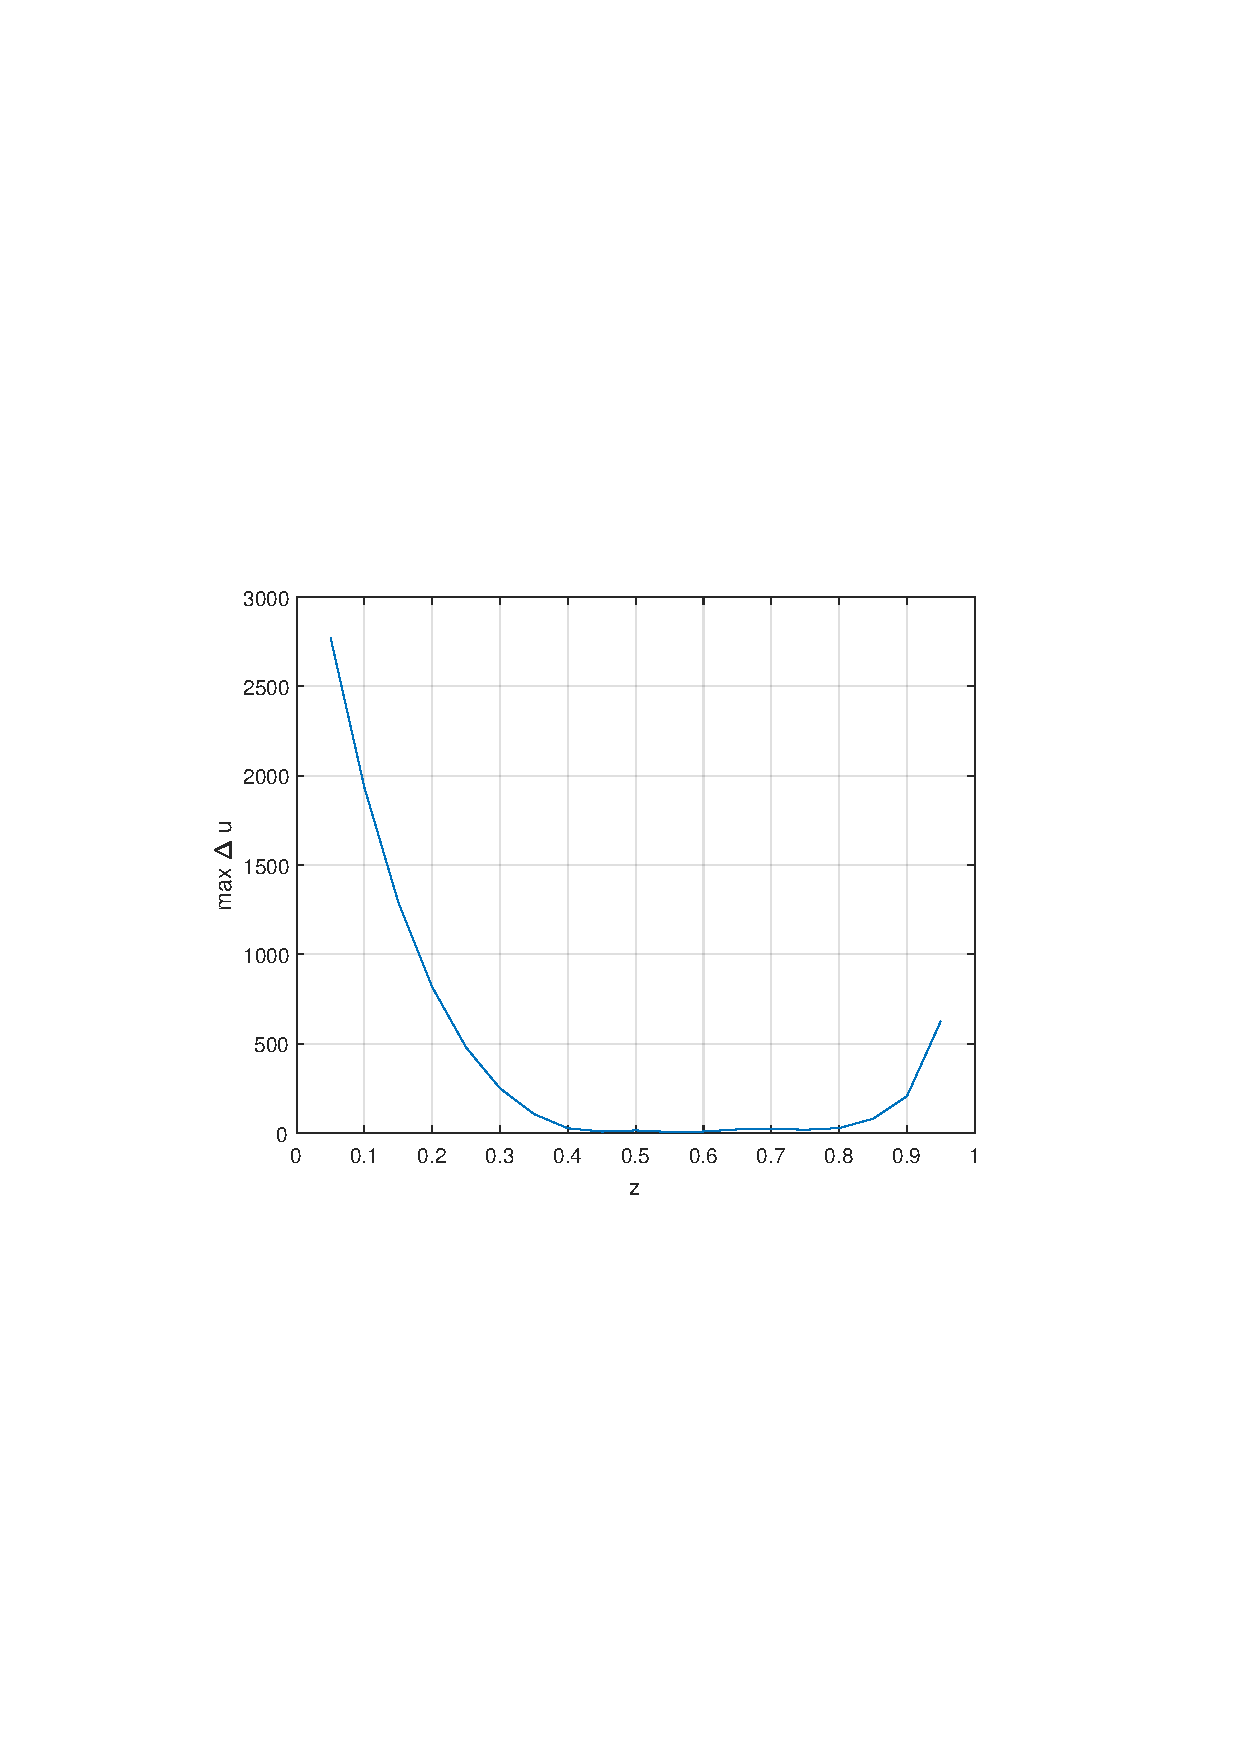
\includegraphics[clip, trim=0.5cm 10cm 0.5cm 9.5cm, width=1.00\textwidth]{../rys/zad3_max_u.pdf}
\label{fig:rys3.1.10}
\caption{Zależność maksymalnego przyrostu sterowania od położenia biegunów}
\end{figure}
\subsubsection{Wnioski}
Z otrzymanych wyników można zauważyć, że układ reaguje najłagodniej dla biegunów równych $0,6$.
Czas regulacji jest zbliżony dla biegunów $0,4 0,5$ i $0,6$. Wraz ze zmniejszaniem wartości biegunów maleje czas regulacji, jednak rośnie przeregulowanie. Najlepszy wydaje się układ z biegunami $z=0,5$. Jest  szybszy od $z=0,6$, a przeregulowanie jest niewiele większe.
\subsection{Zadanie b)}
\subsubsection{Wykresy}
\vbox{
\begin{figure}[H]
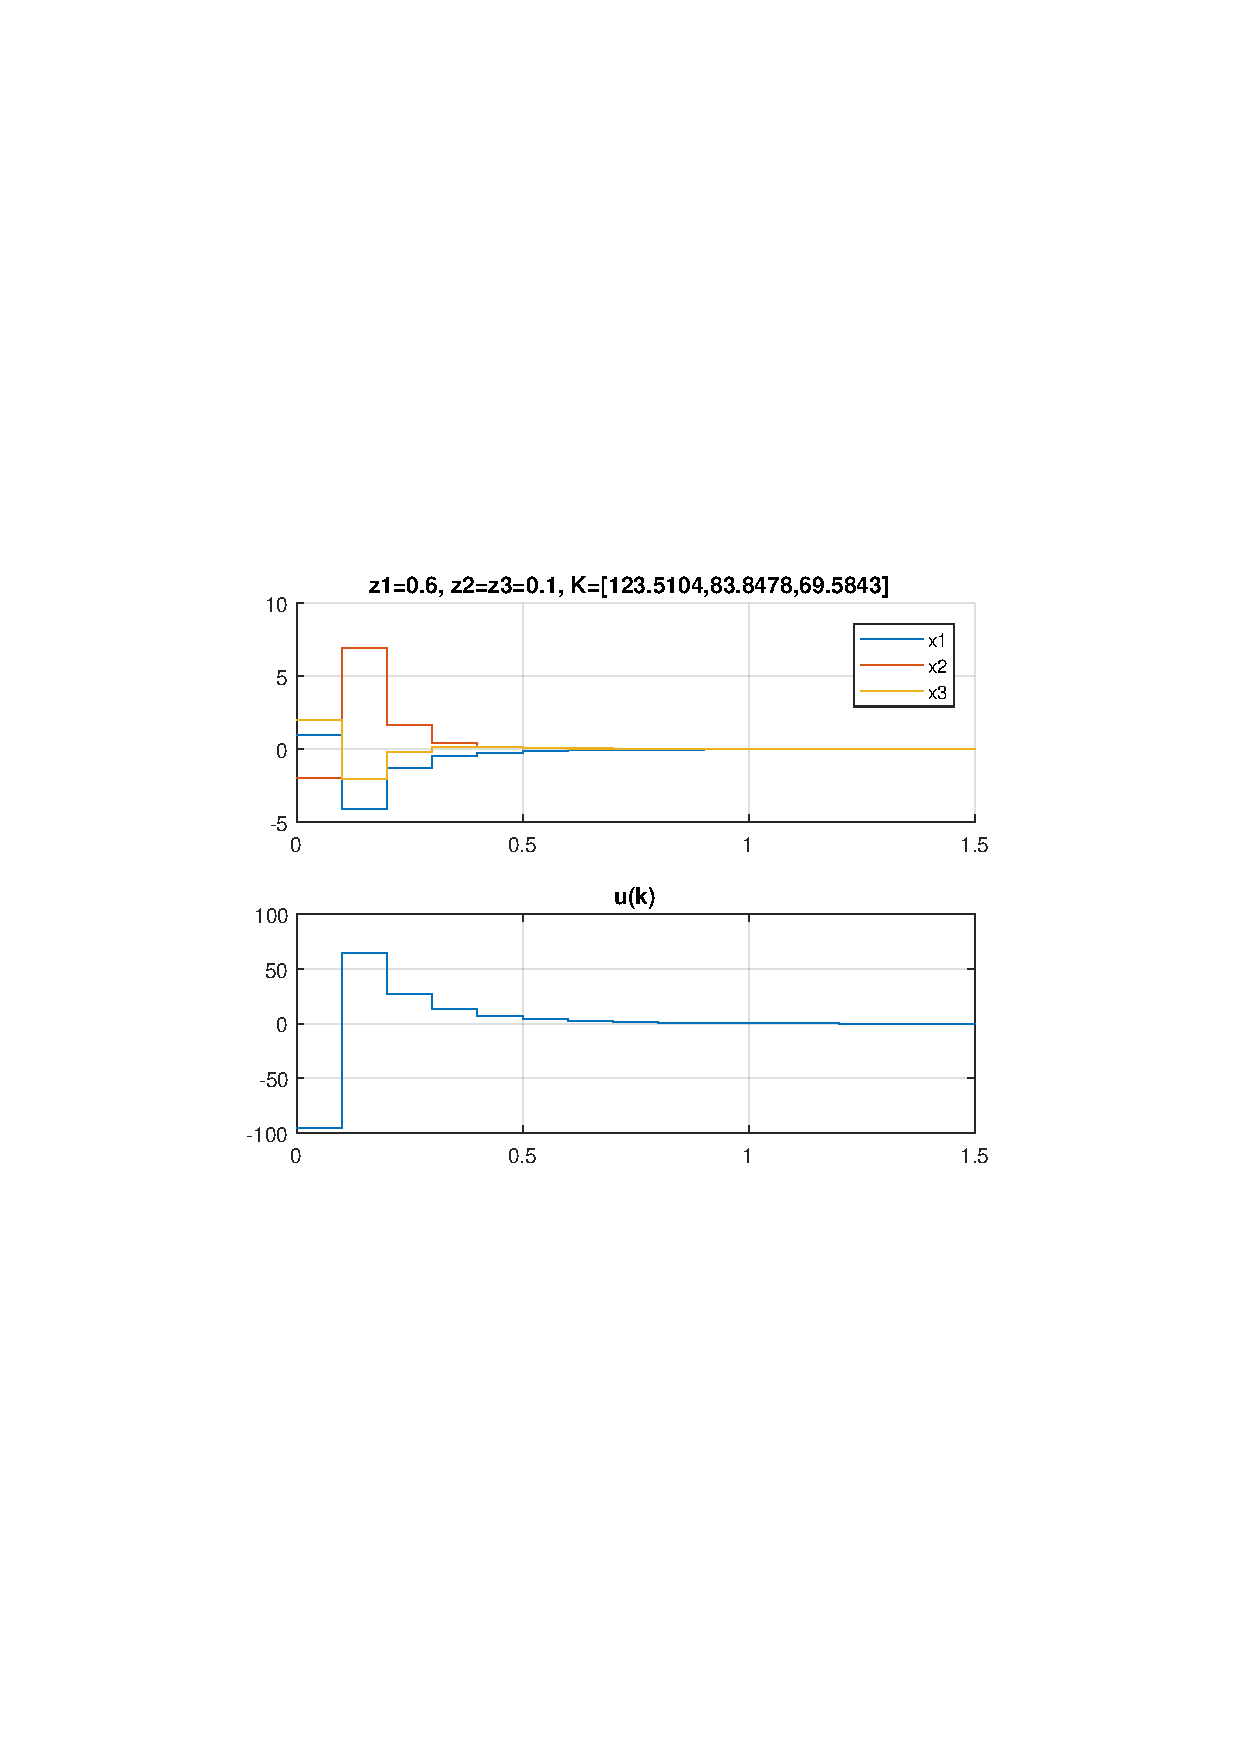
\includegraphics[clip, trim=0.5cm 9.5cm 0.5cm 9.5cm, width=1.00\textwidth]{../rys/zad3b_rys1.pdf}
\label{fig:rys3.2.1}
\caption{2.1}
\end{figure}

\begin{figure}[H]
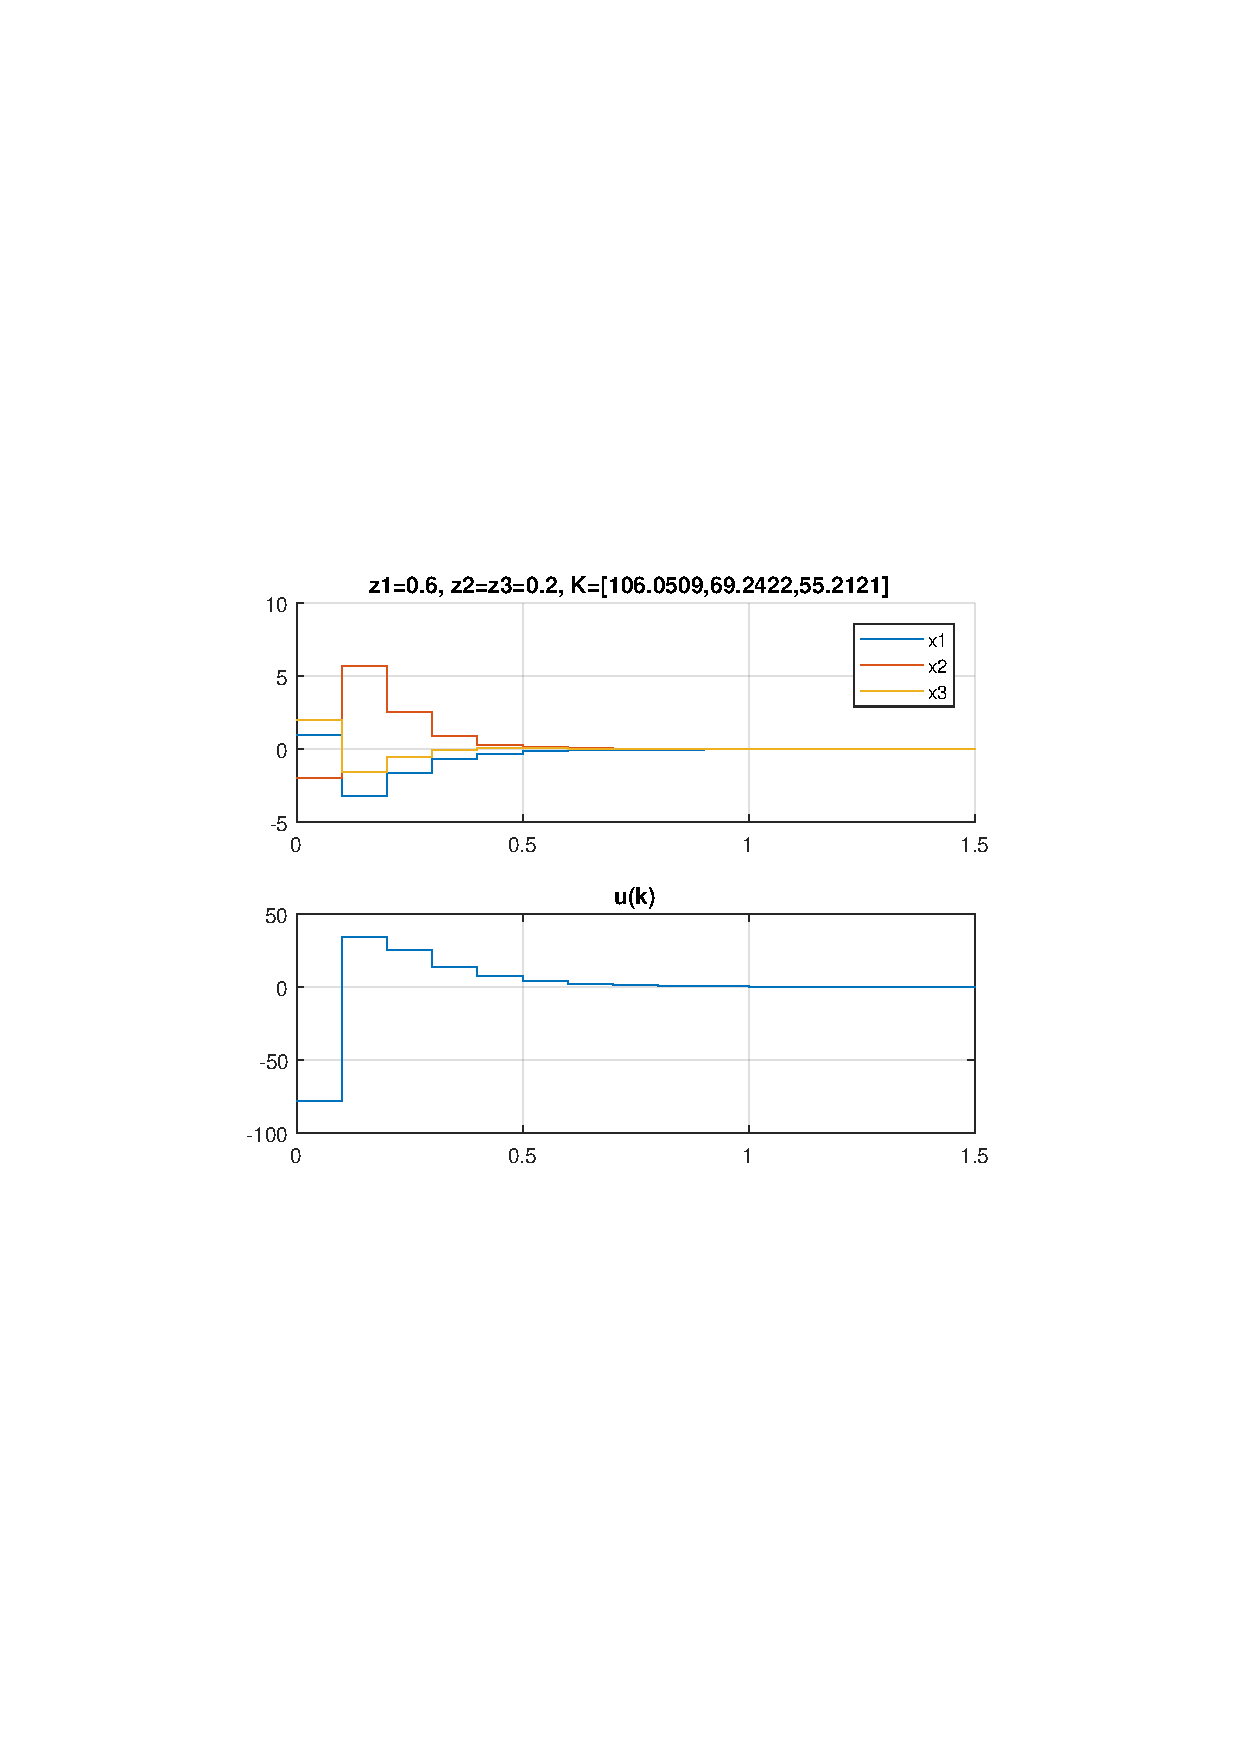
\includegraphics[clip, trim=0.5cm 9.5cm 0.5cm 9.5cm, width=1.00\textwidth]{../rys/zad3b_rys2.pdf}
\label{fig:rys3.2.2}
\caption{2.2}
\end{figure}
}
\vbox{
\begin{figure}[H]
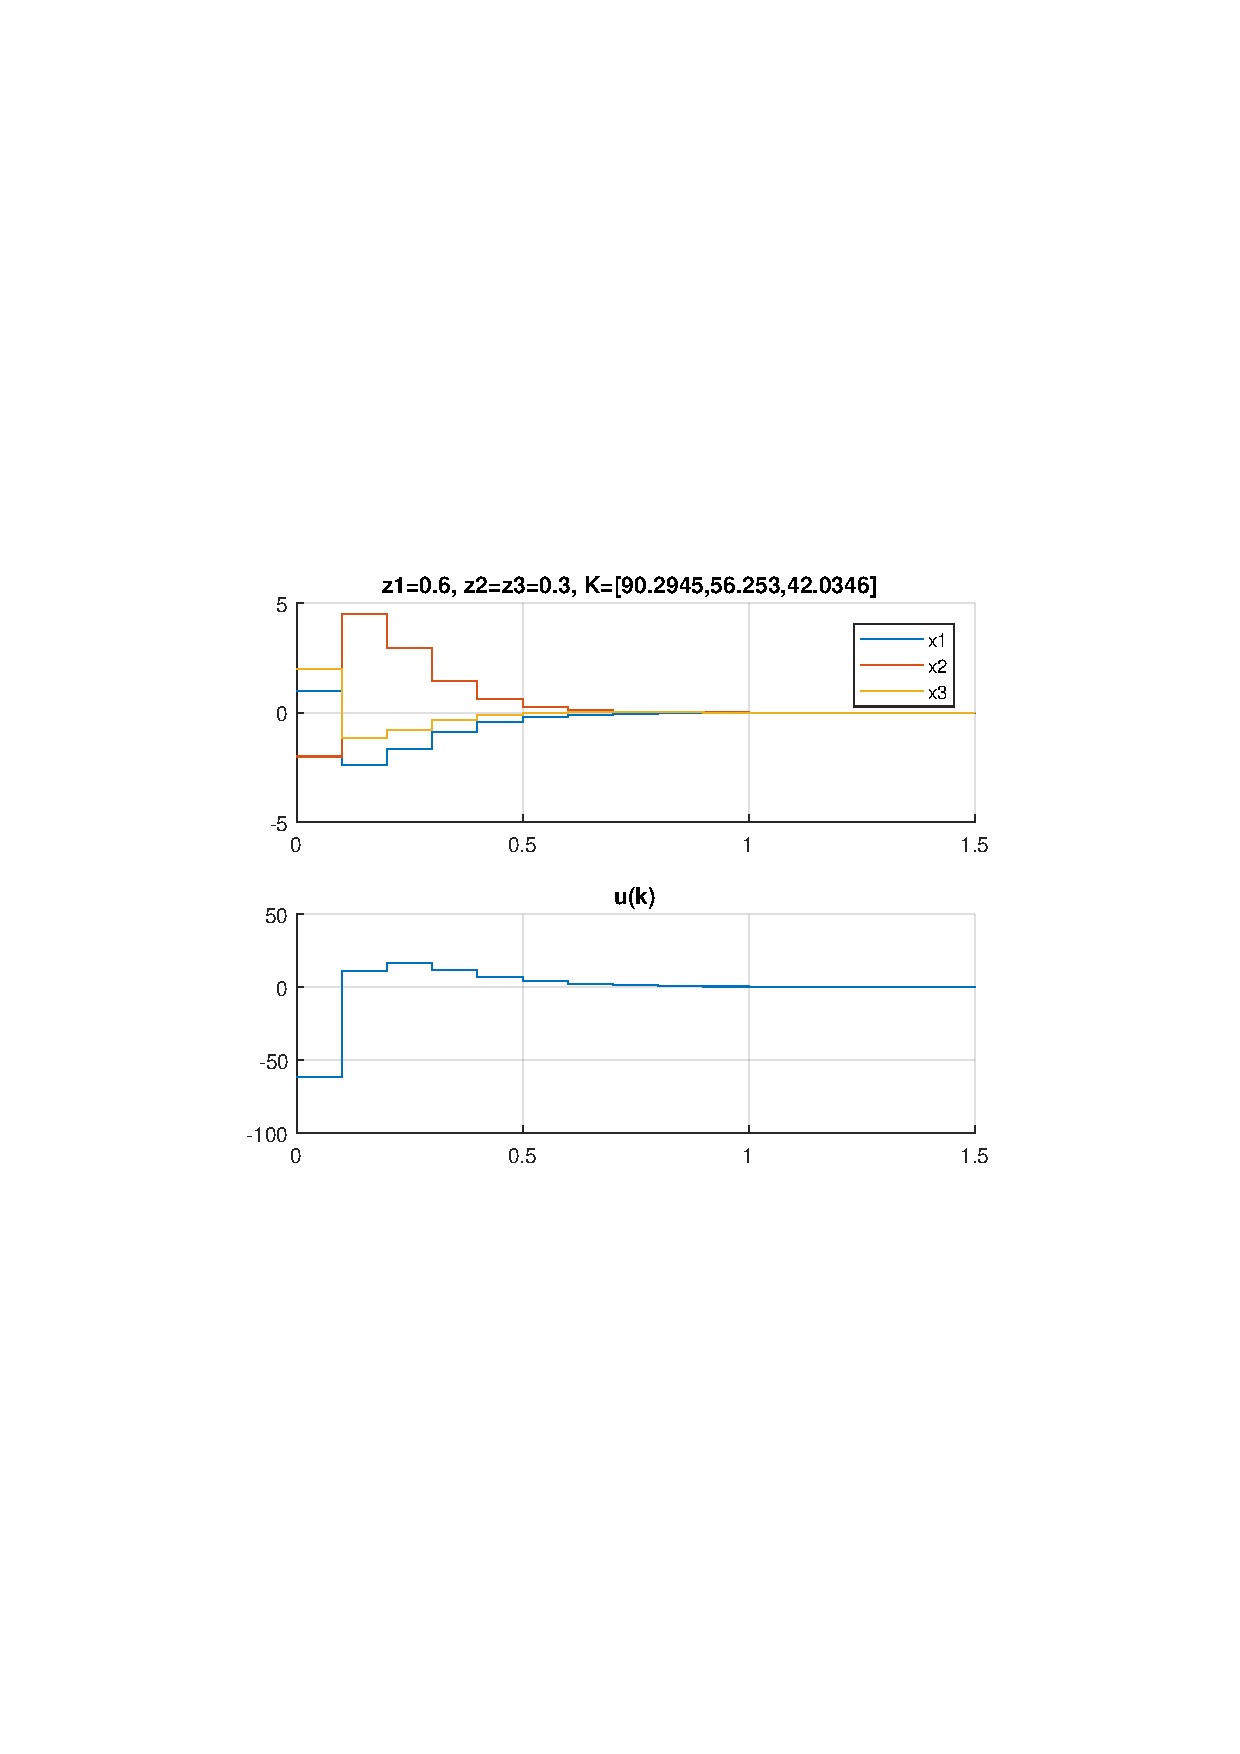
\includegraphics[clip, trim=0.5cm 9.5cm 0.5cm 9.5cm, width=1.00\textwidth]{../rys/zad3b_rys3.pdf}
\label{fig:rys3.2.3}
\caption{2.3}
\end{figure}

\begin{figure}[H]
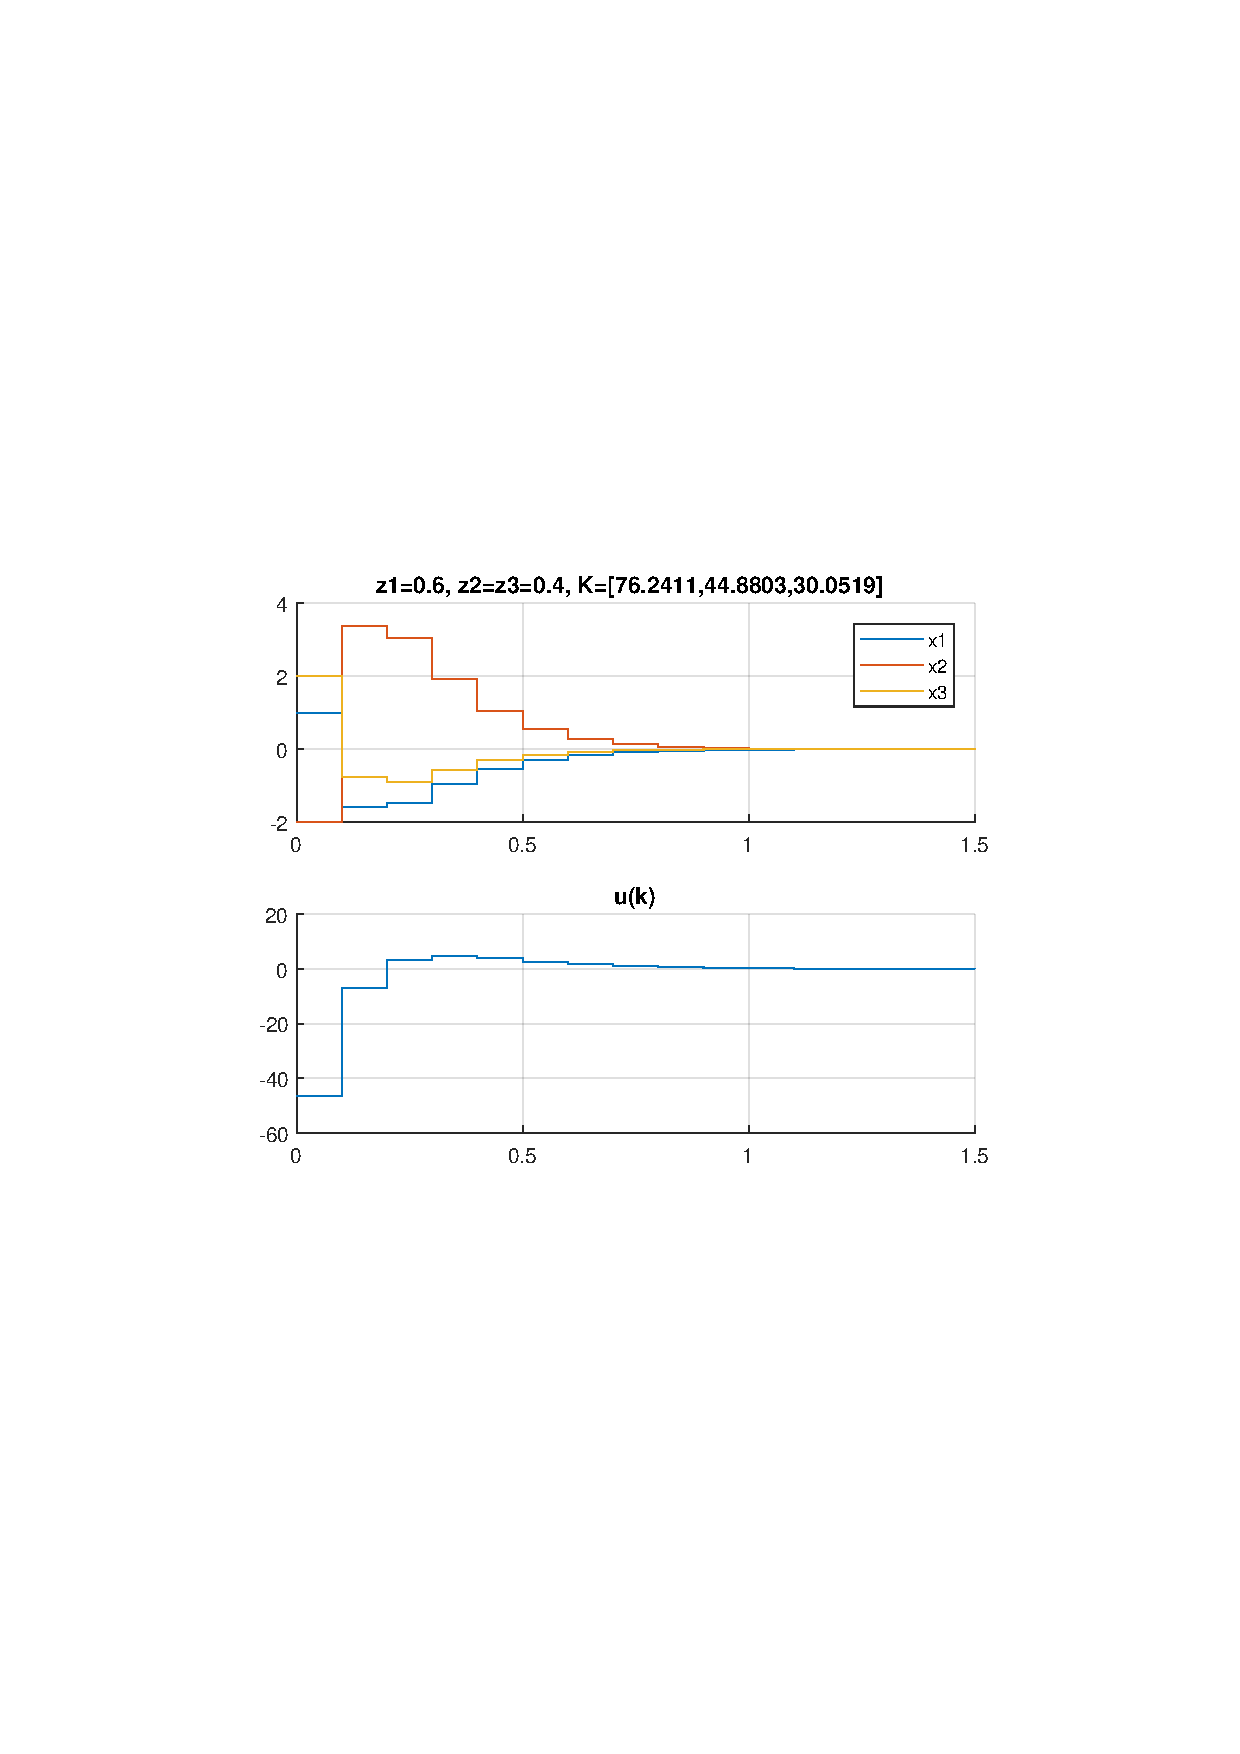
\includegraphics[clip, trim=0.5cm 9.5cm 0.5cm 9.5cm, width=1.00\textwidth]{../rys/zad3b_rys4.pdf}
\label{fig:rys3.2.4}
\caption{2.4}
\end{figure}
}
\vbox{
\begin{figure}[H]
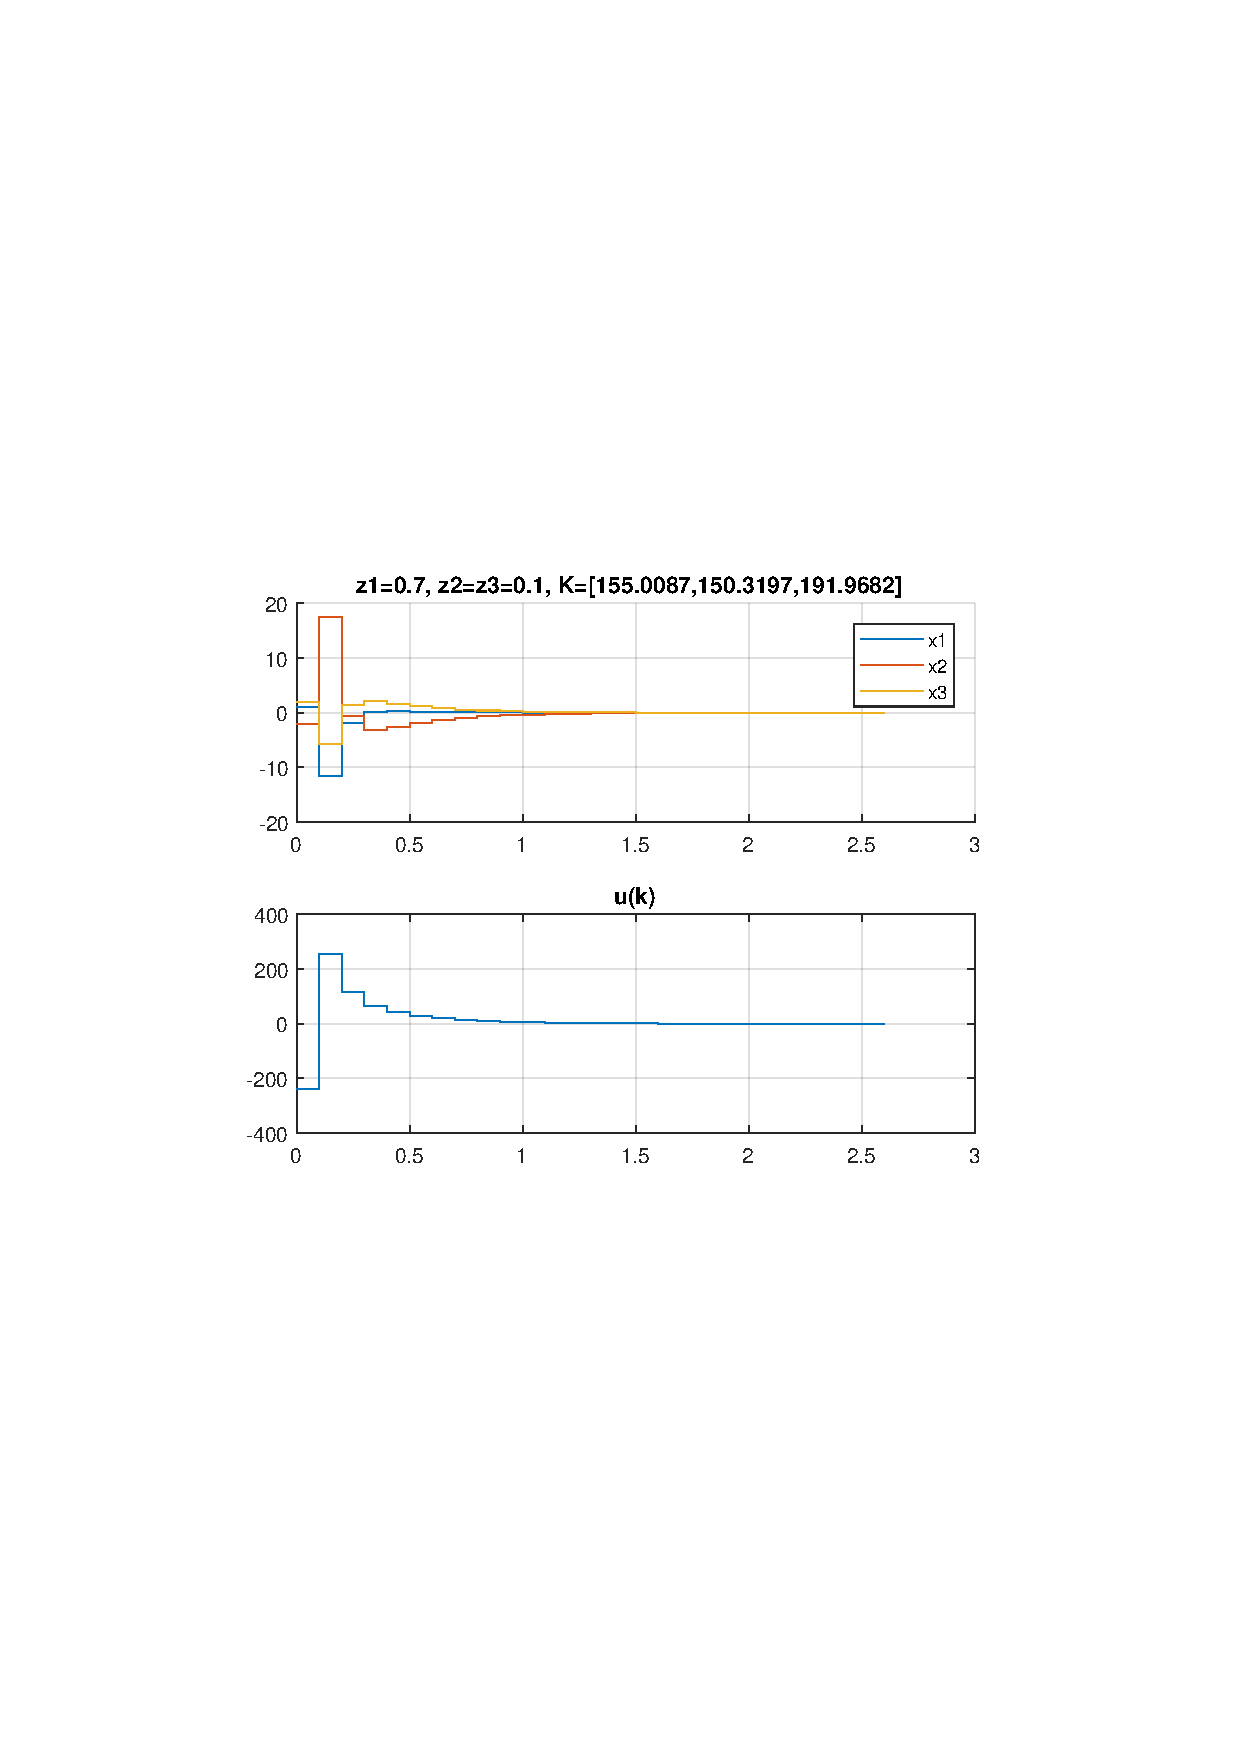
\includegraphics[clip, trim=0.5cm 9.5cm 0.5cm 9.5cm, width=1.00\textwidth]{../rys/zad3b_rys5.pdf}
\label{fig:rys3.2.5}
\caption{2.5}
\end{figure}

\begin{figure}[H]
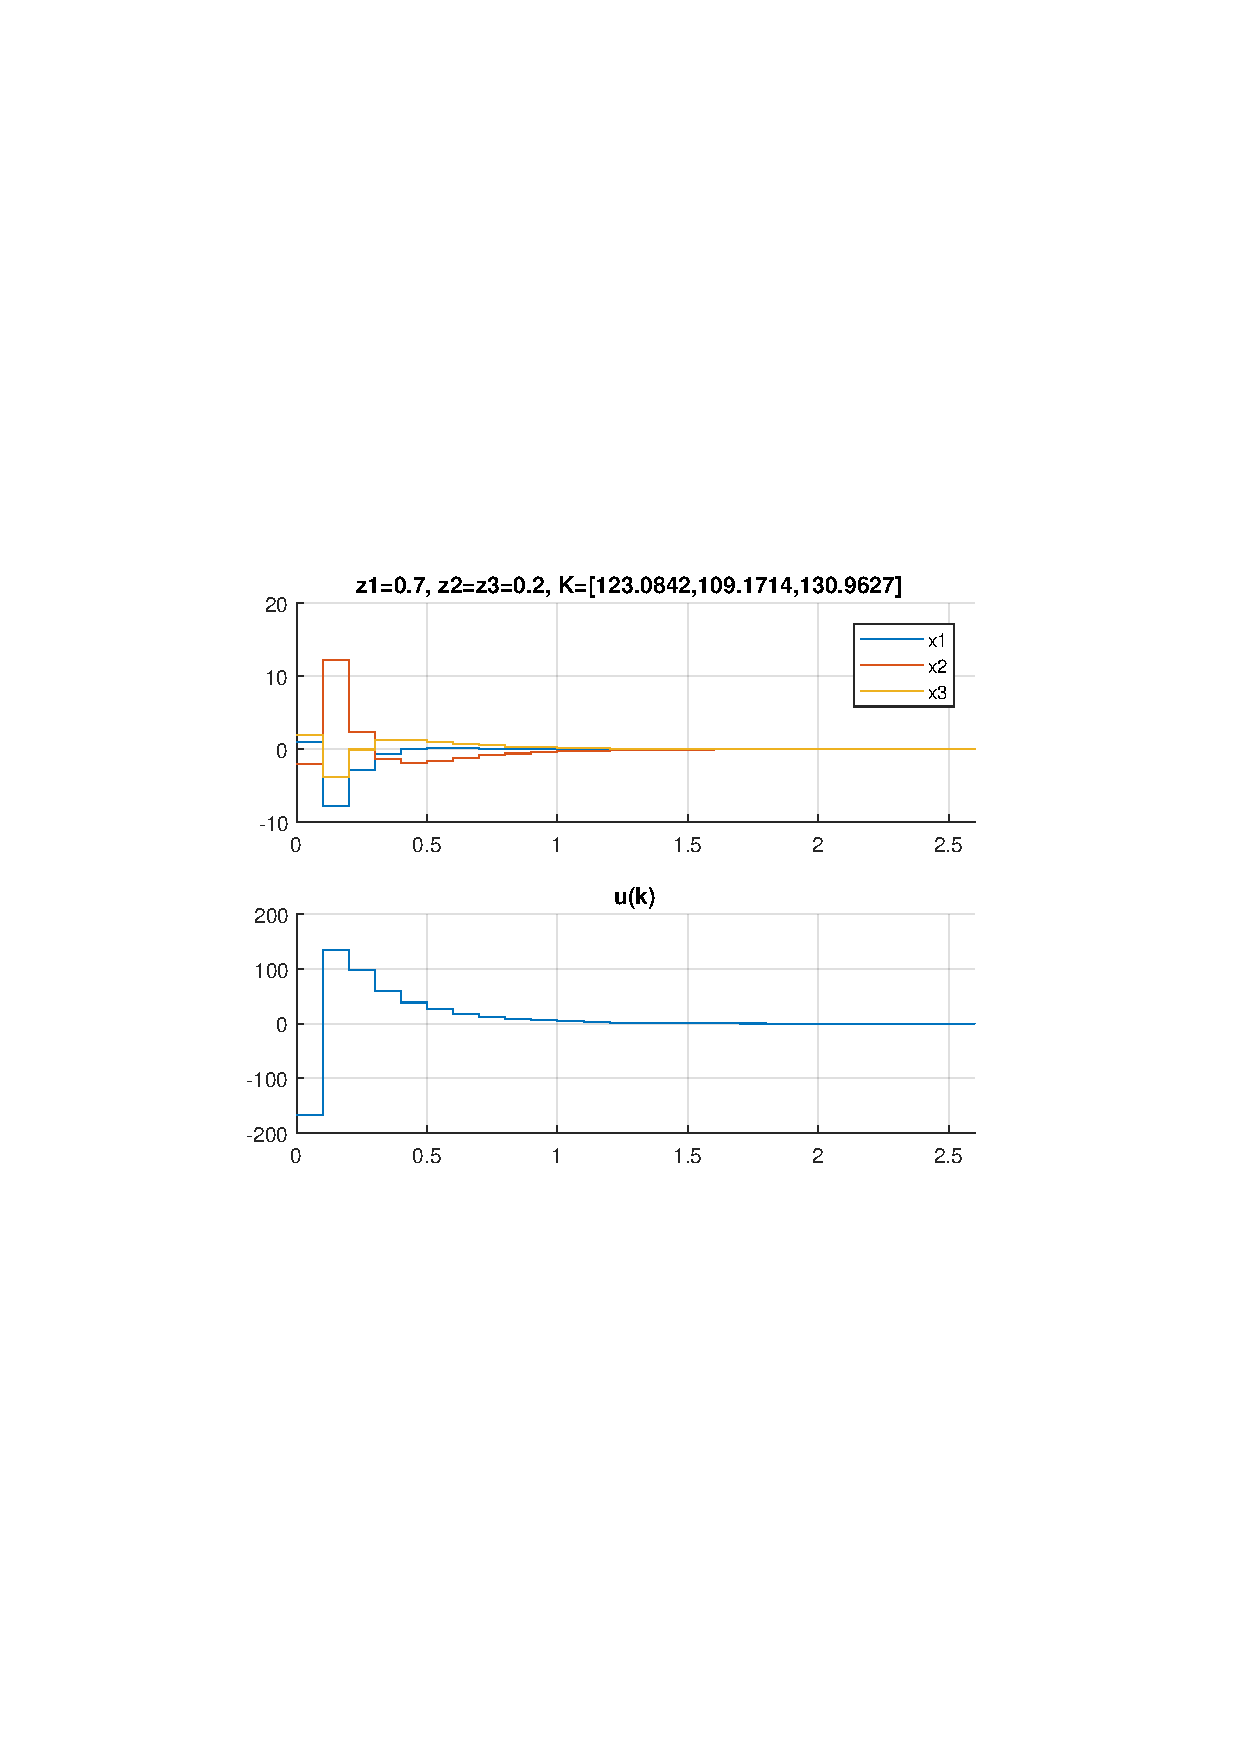
\includegraphics[clip, trim=0.5cm 9.5cm 0.5cm 9.5cm, width=1.00\textwidth]{../rys/zad3b_rys6.pdf}
\label{fig:rys3.2.6}
\caption{2.6}
\end{figure}
}
\vbox{
\begin{figure}[H]
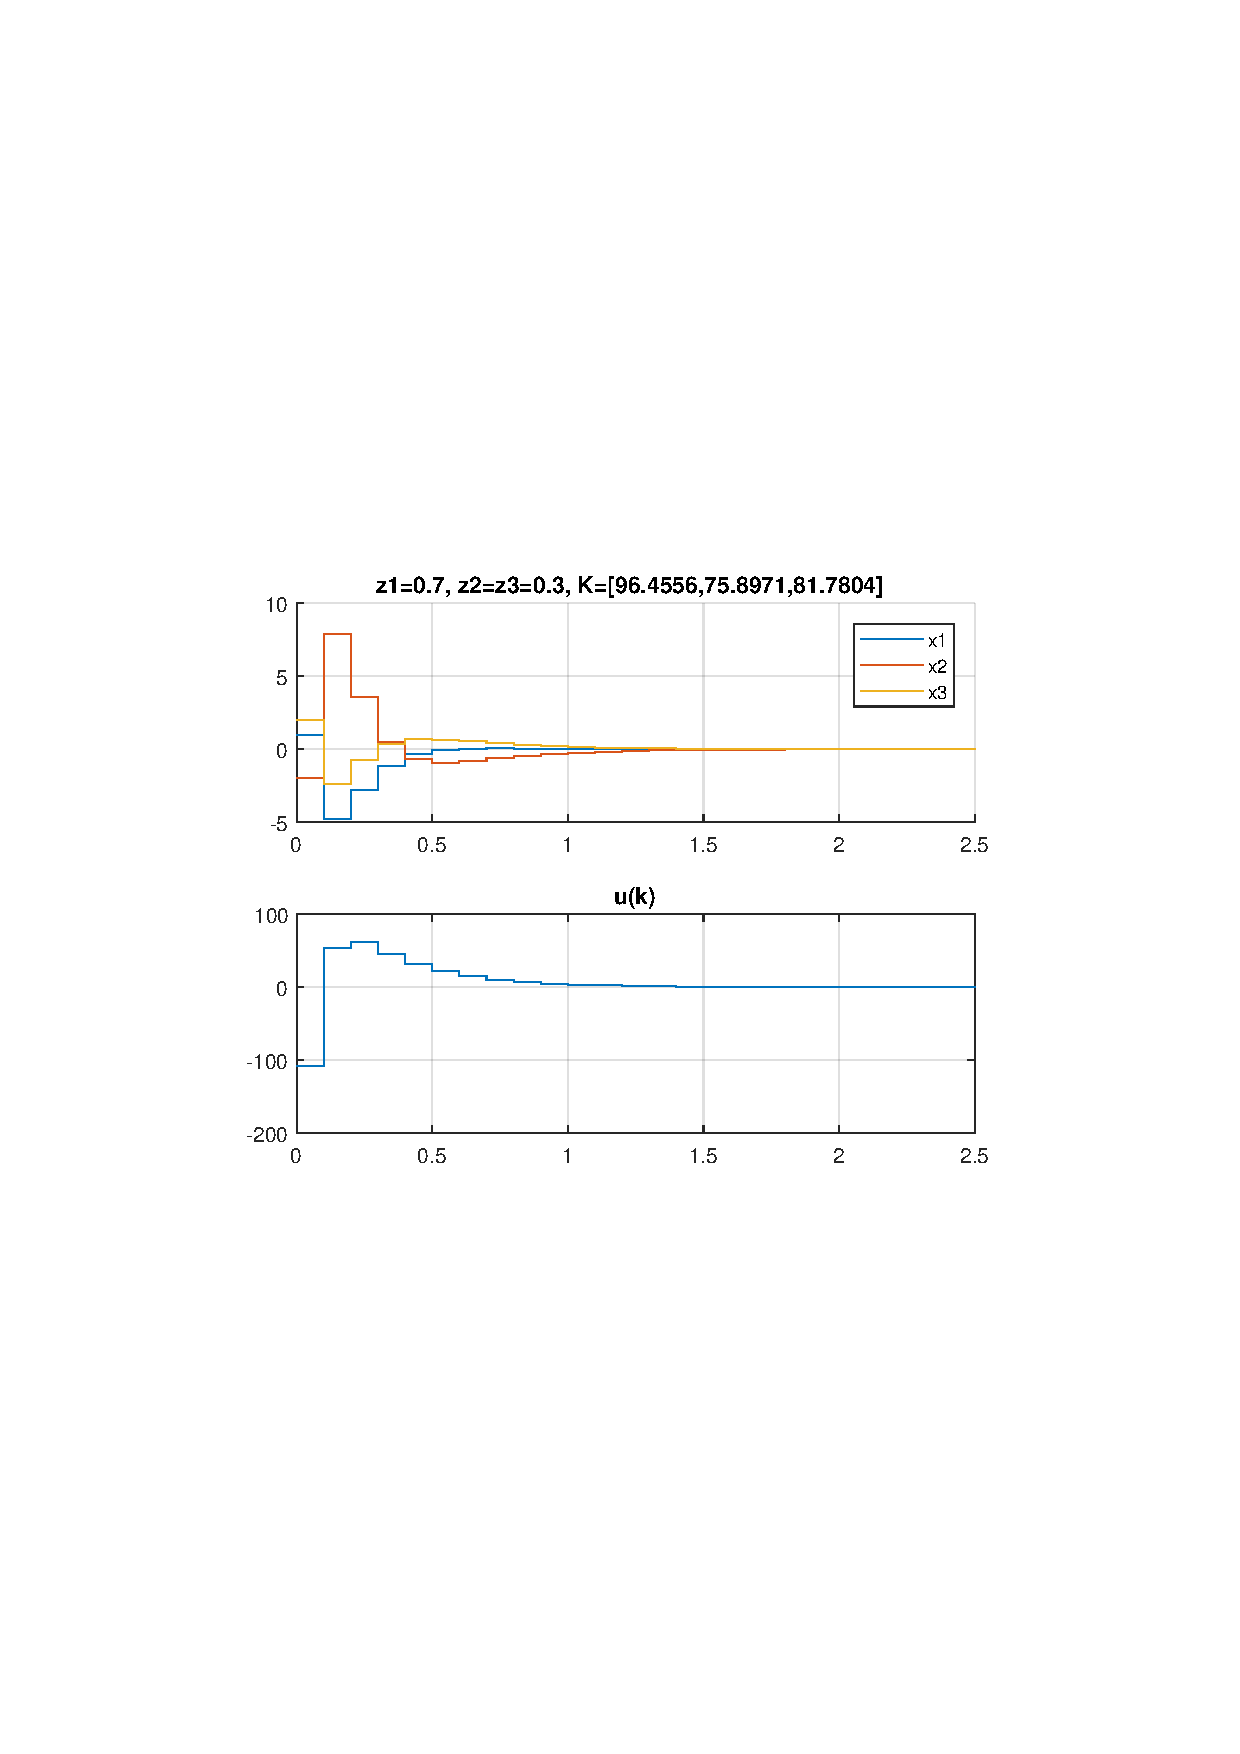
\includegraphics[clip, trim=0.5cm 9.5cm 0.5cm 9.5cm, width=1.00\textwidth]{../rys/zad3b_rys7.pdf}
\label{fig:rys3.2.7}
\caption{2.7}
\end{figure}

\begin{figure}[H]
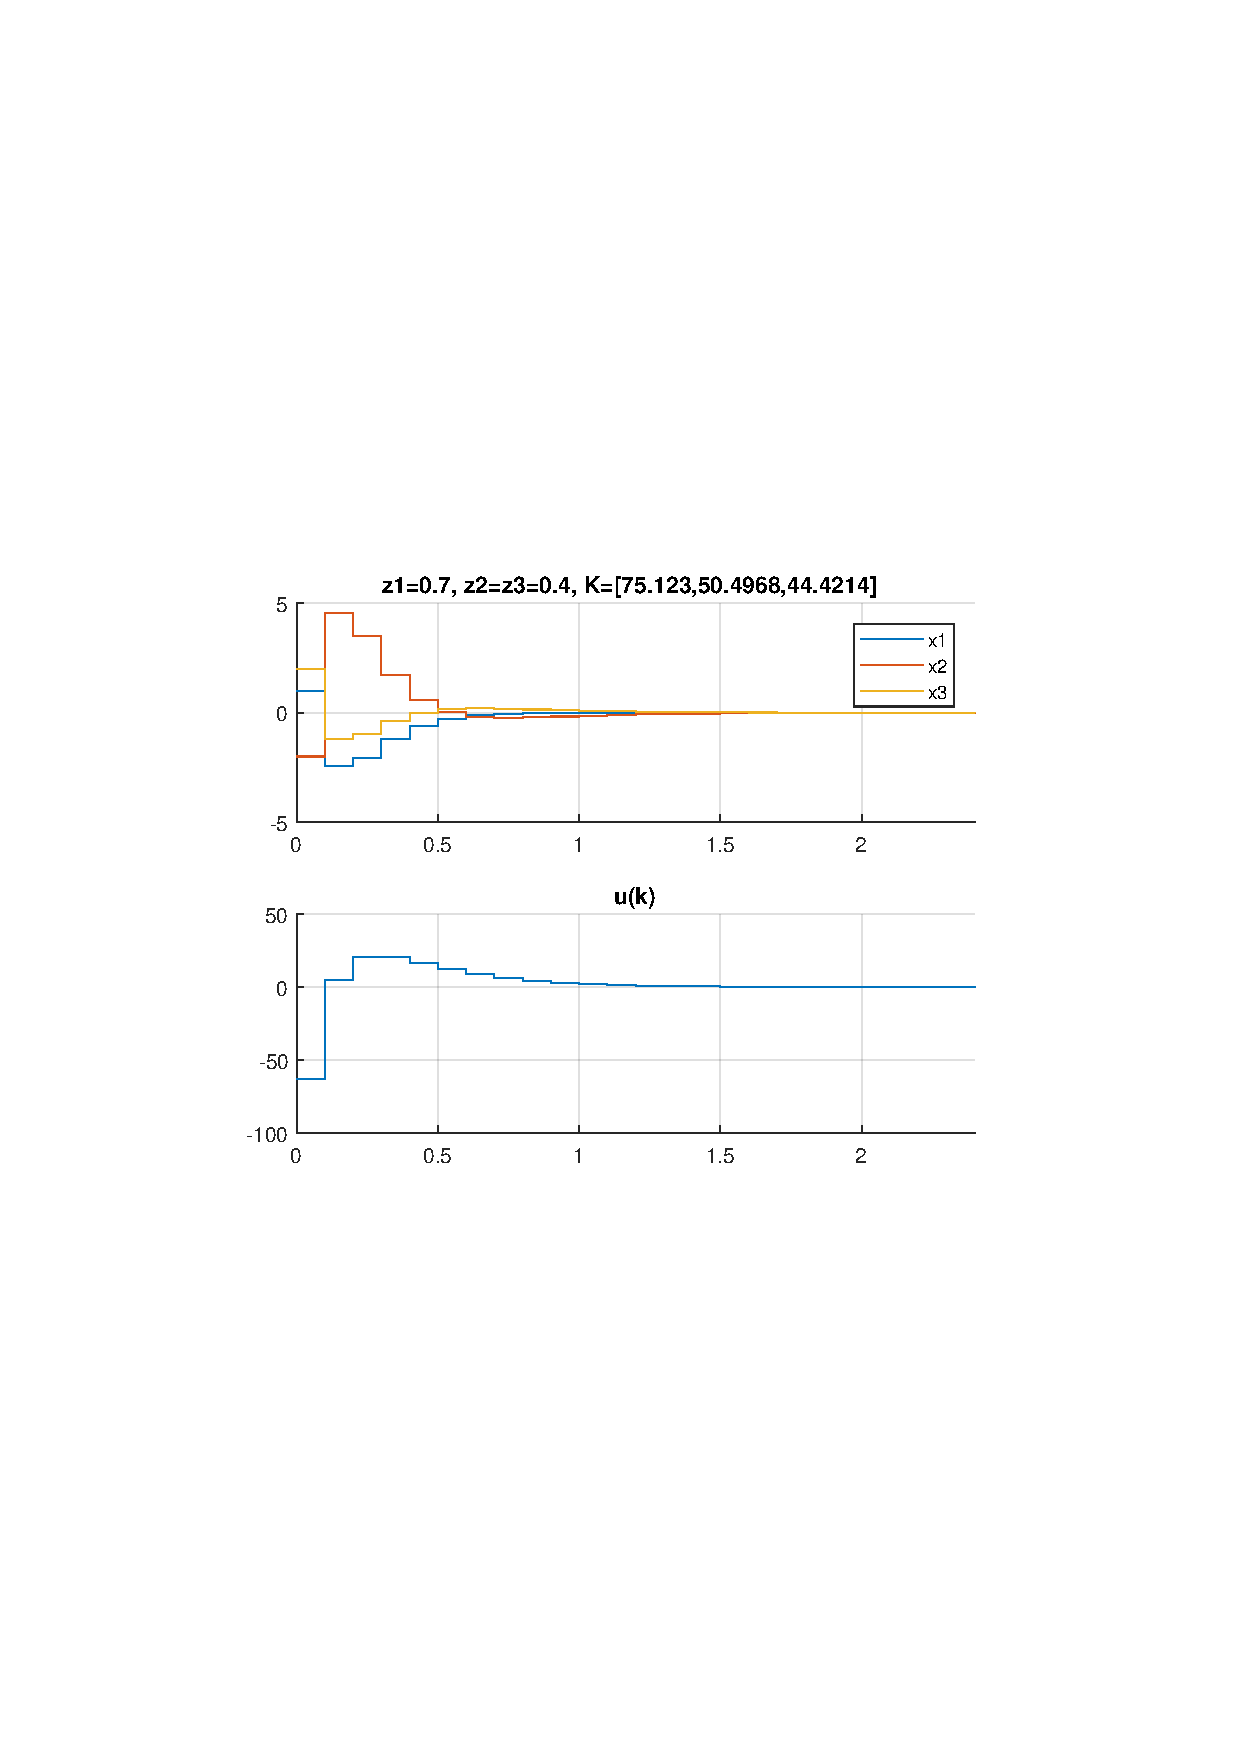
\includegraphics[clip, trim=0.5cm 9.5cm 0.5cm 9.5cm, width=1.00\textwidth]{../rys/zad3b_rys8.pdf}
\label{fig:rys3.2.8}
\caption{2.8}
\end{figure}
}
\vbox{
\begin{figure}[H]
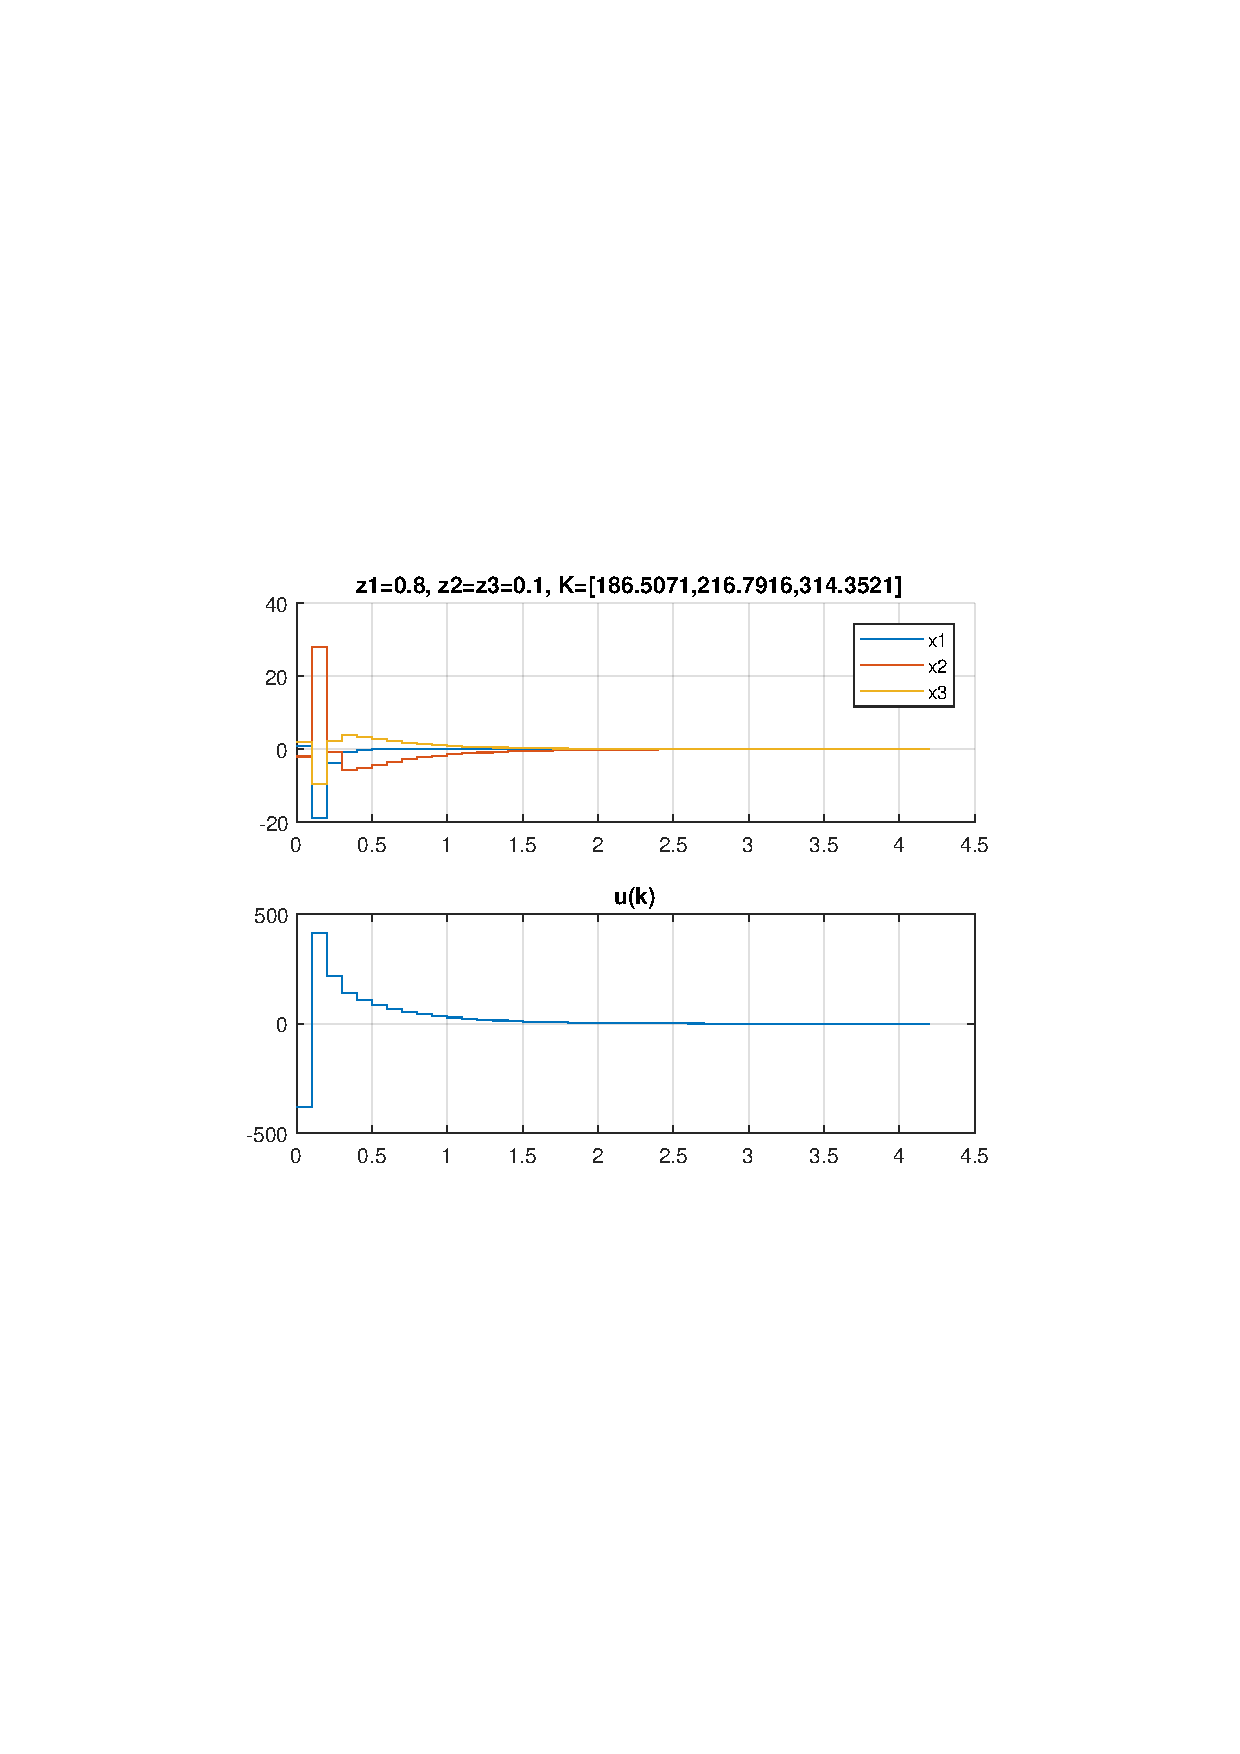
\includegraphics[clip, trim=0.5cm 9.5cm 0.5cm 9.5cm, width=1.00\textwidth]{../rys/zad3b_rys9.pdf}
\label{fig:rys3.2.9}
\caption{2.9}
\end{figure}

\begin{figure}[H]
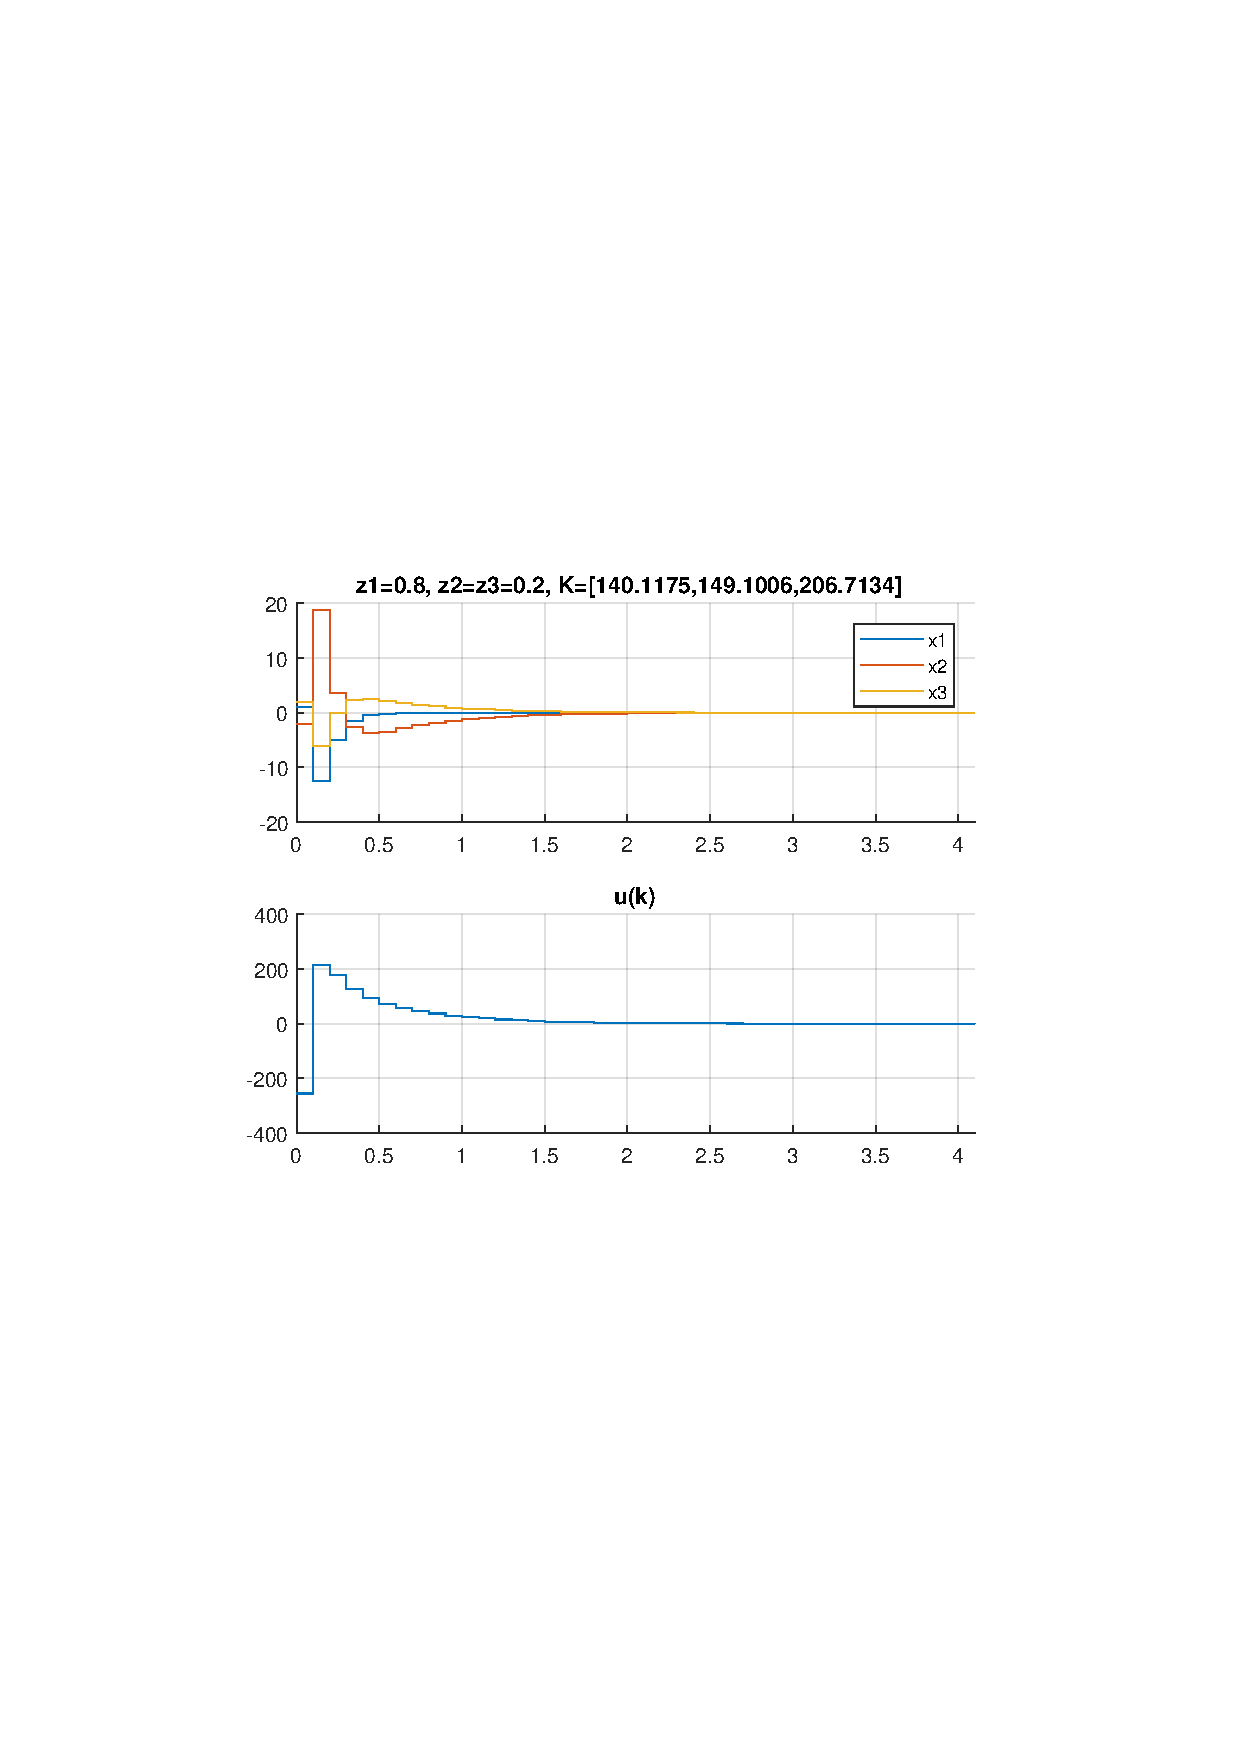
\includegraphics[clip, trim=0.5cm 9.5cm 0.5cm 9.5cm, width=1.00\textwidth]{../rys/zad3b_rys10.pdf}
\label{fig:rys3.2.10}
\caption{2.10}
\end{figure}
}
\vbox{
\begin{figure}[H]
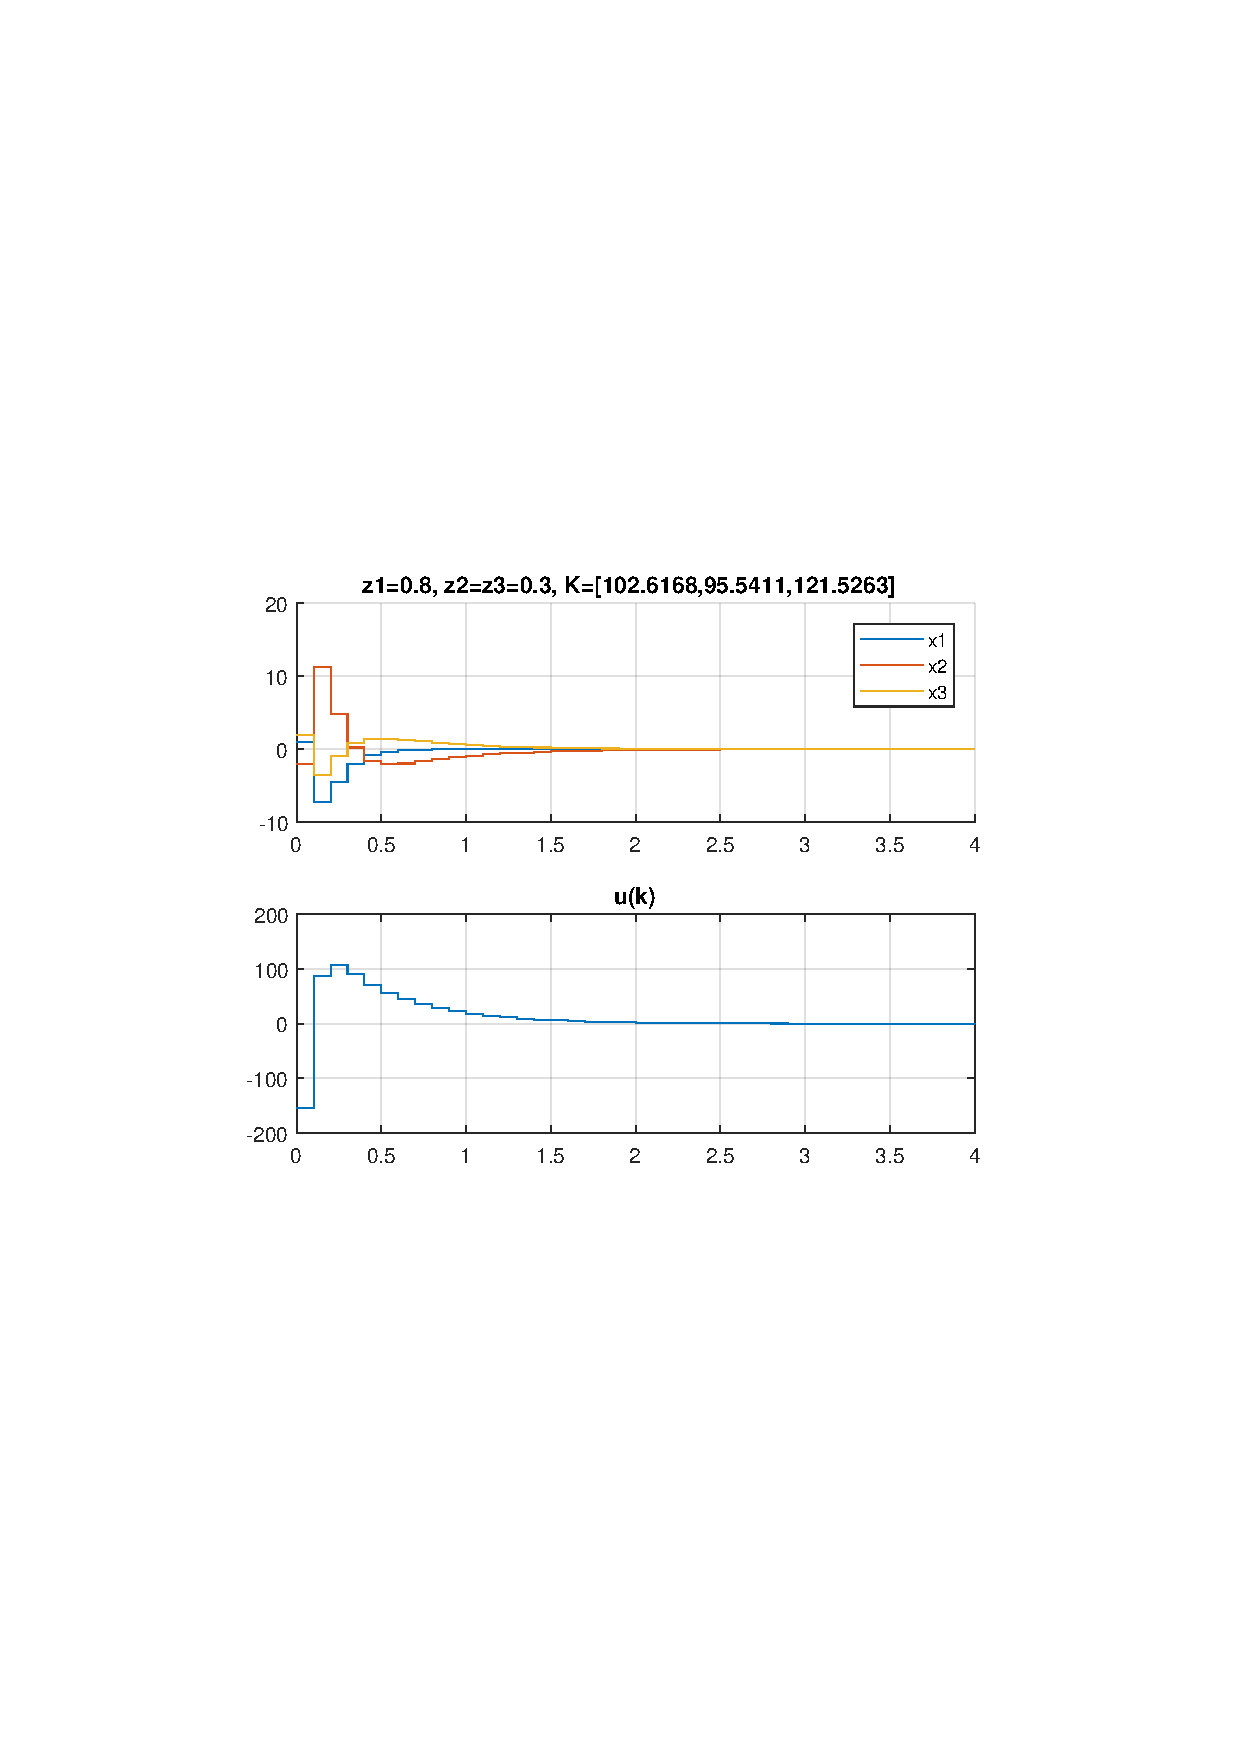
\includegraphics[clip, trim=0.5cm 9.5cm 0.5cm 9.5cm, width=1.00\textwidth]{../rys/zad3b_rys11.pdf}
\label{fig:rys3.2.11}
\caption{2.11}
\end{figure}

\begin{figure}[H]
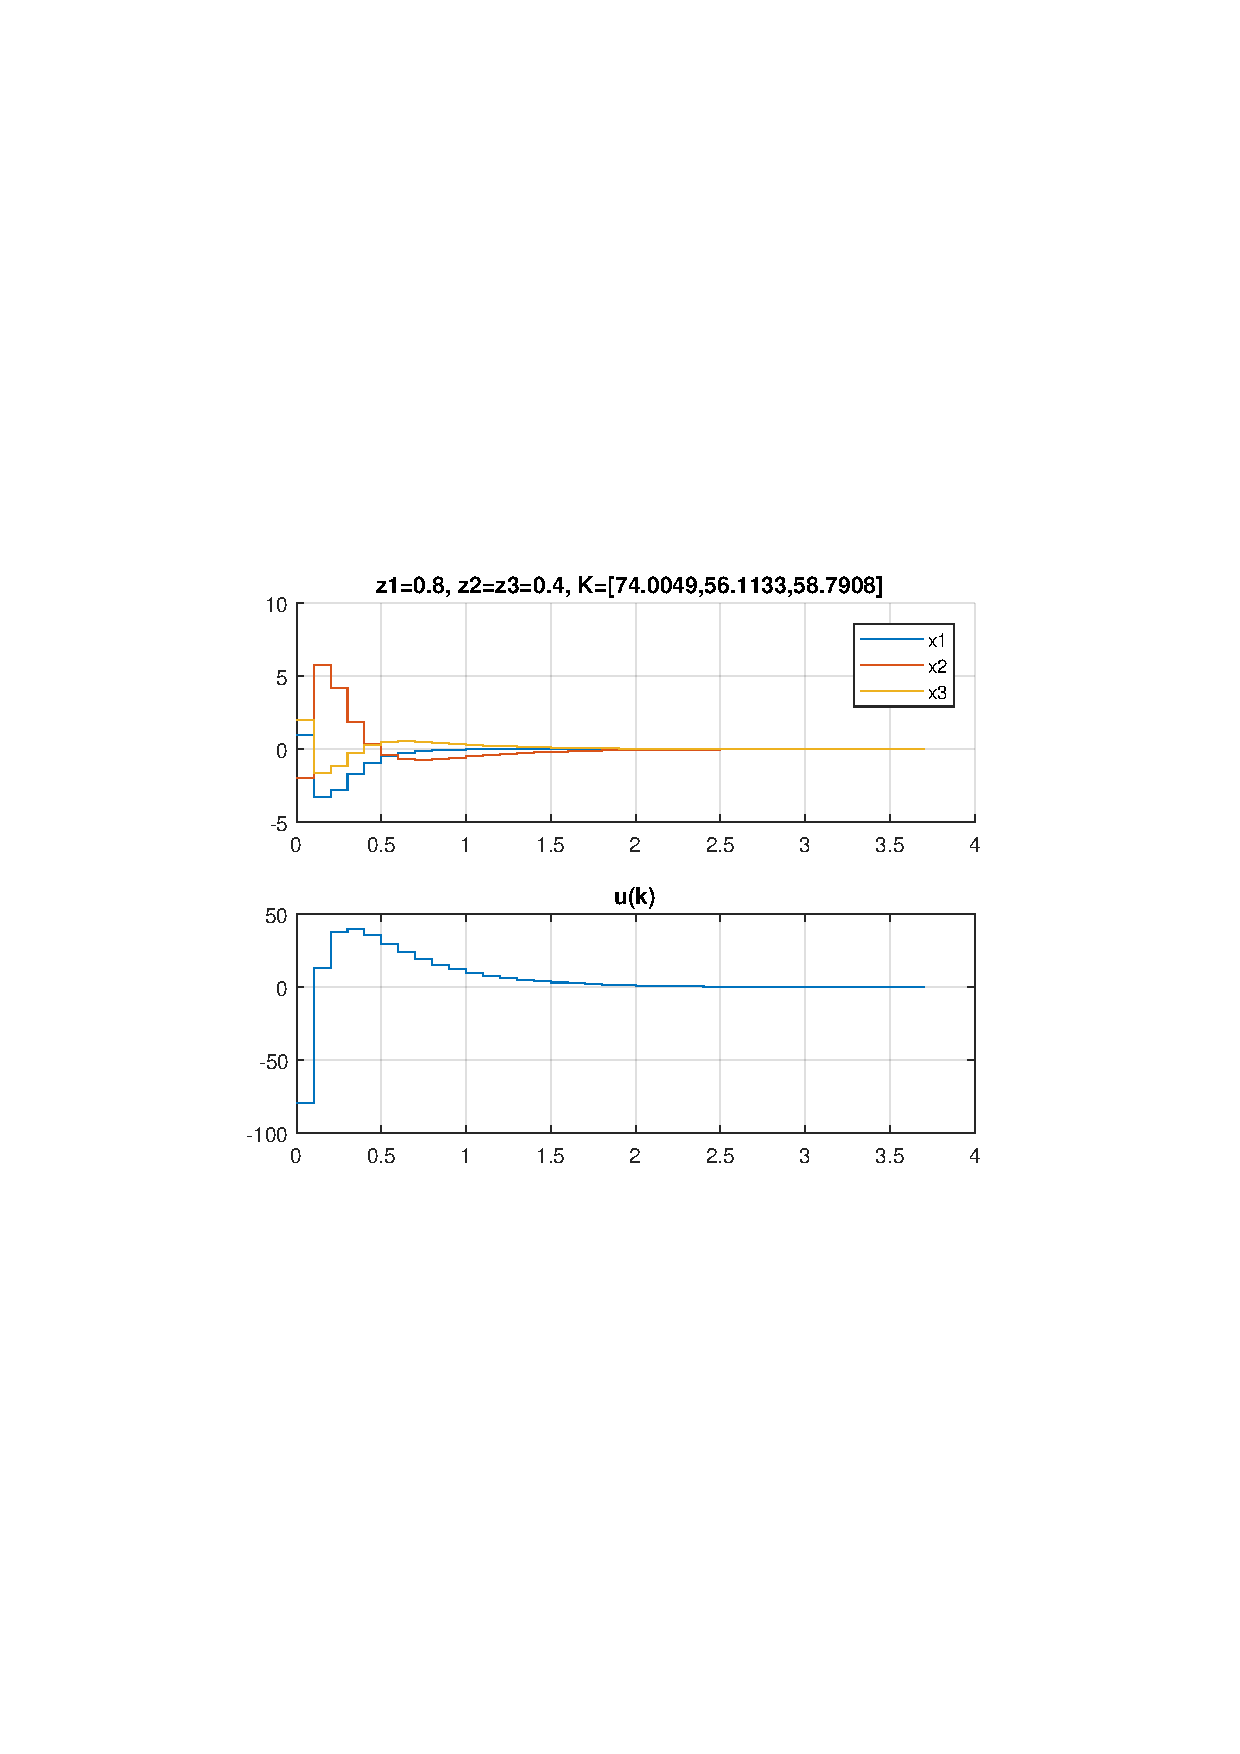
\includegraphics[clip, trim=0.5cm 9.5cm 0.5cm 9.5cm, width=1.00\textwidth]{../rys/zad3b_rys12.pdf}
\label{fig:rys3.2.12}
\caption{2.12}
\end{figure}
}
\vbox{
\begin{figure}[H]
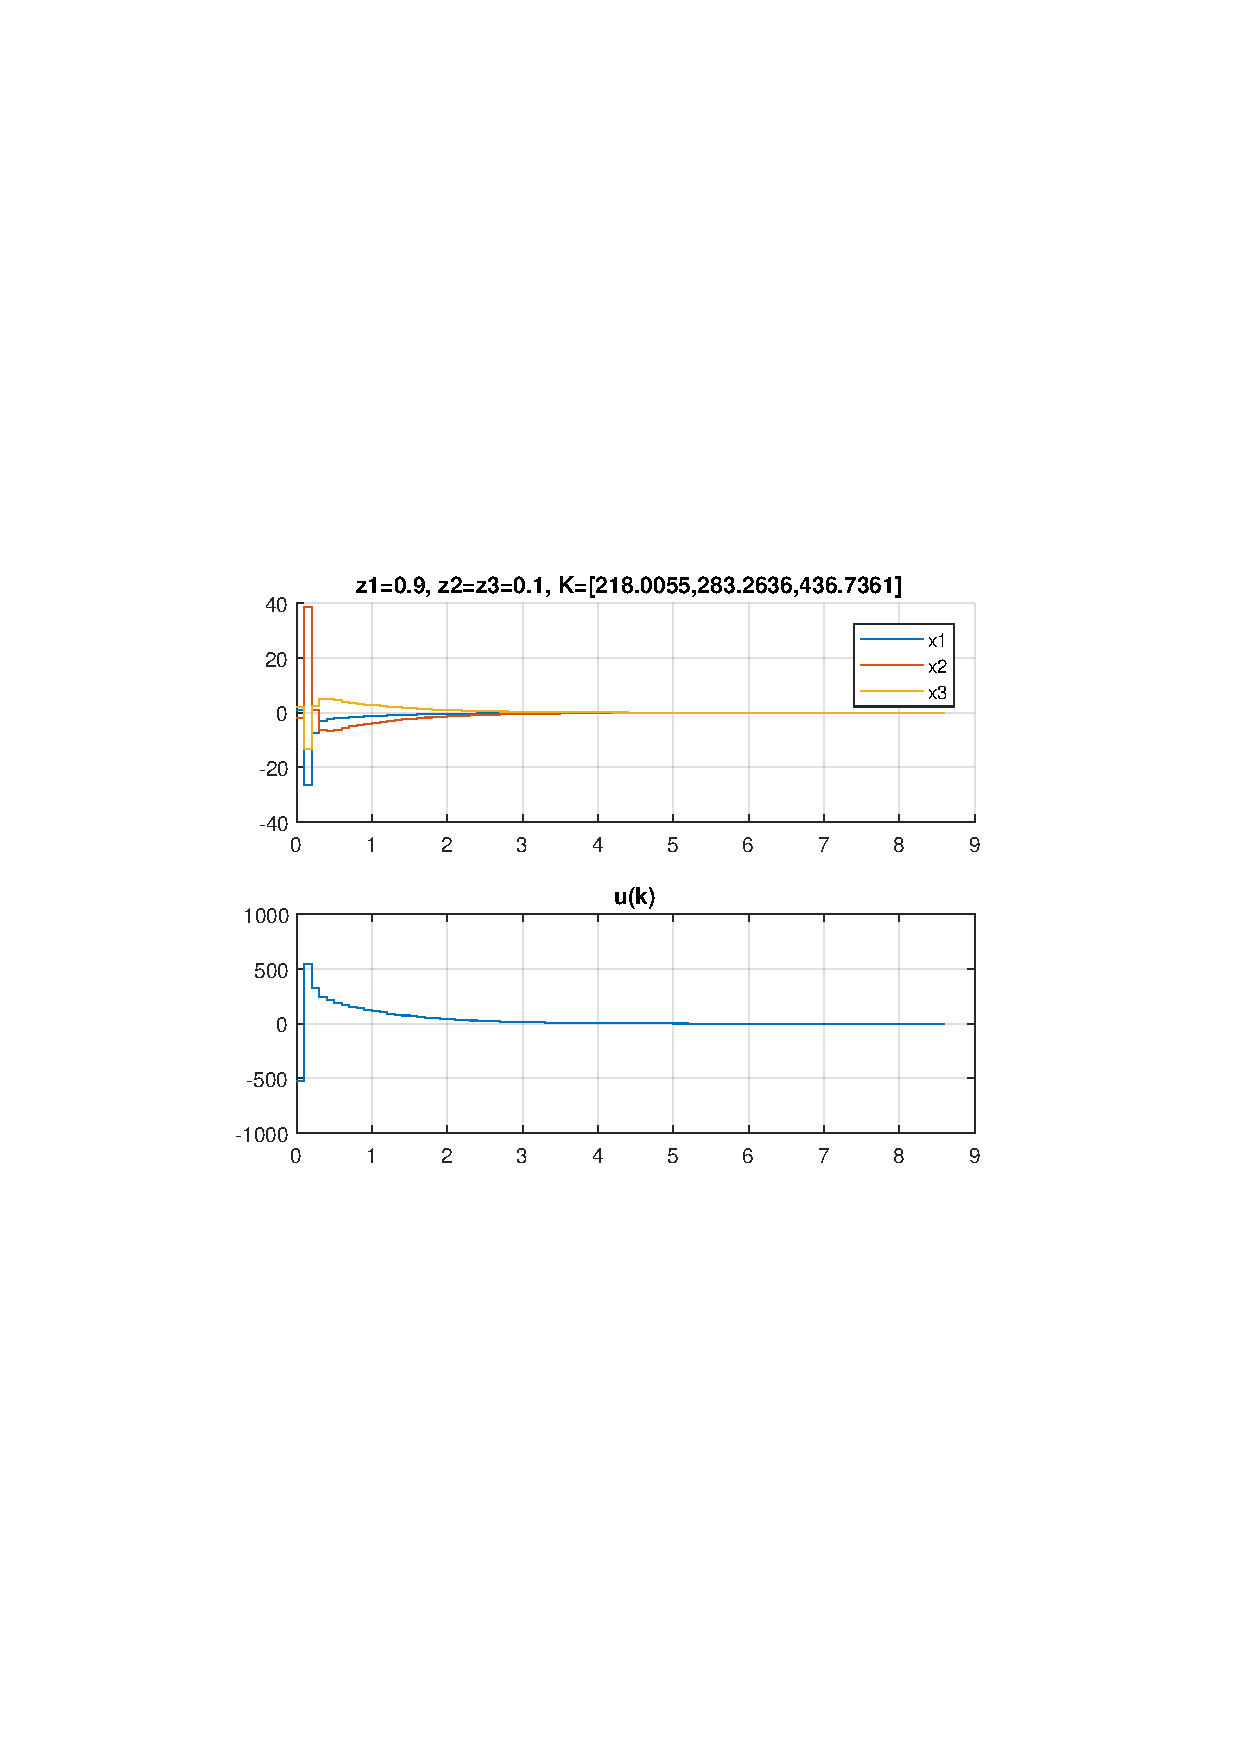
\includegraphics[clip, trim=0.5cm 9.5cm 0.5cm 9.5cm, width=1.00\textwidth]{../rys/zad3b_rys13.pdf}
\label{fig:rys3.2.13}
\caption{2.13}
\end{figure}

\begin{figure}[H]
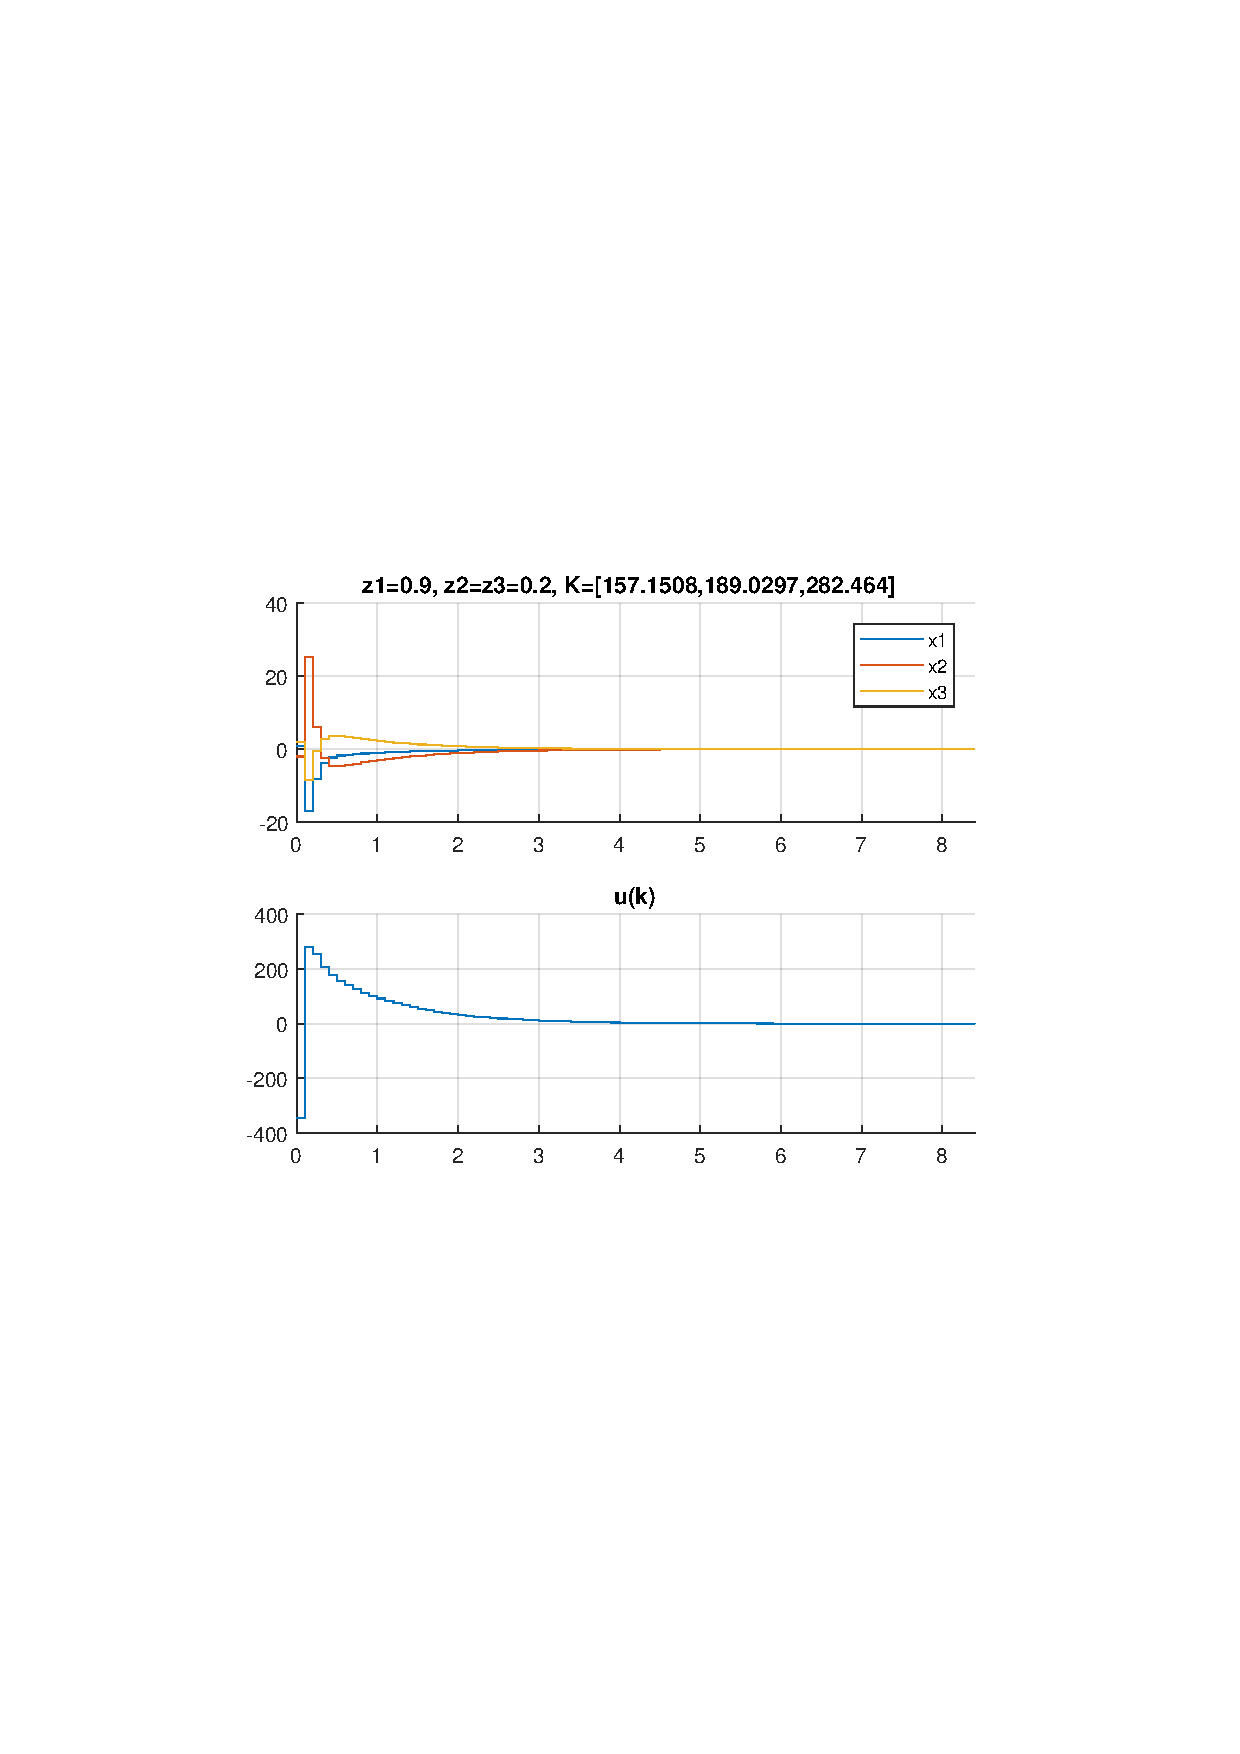
\includegraphics[clip, trim=0.5cm 9.5cm 0.5cm 9.5cm, width=1.00\textwidth]{../rys/zad3b_rys14.pdf}
\label{fig:rys3.2.14}
\caption{2.14}
\end{figure}
}
\vbox{
\begin{figure}[H]
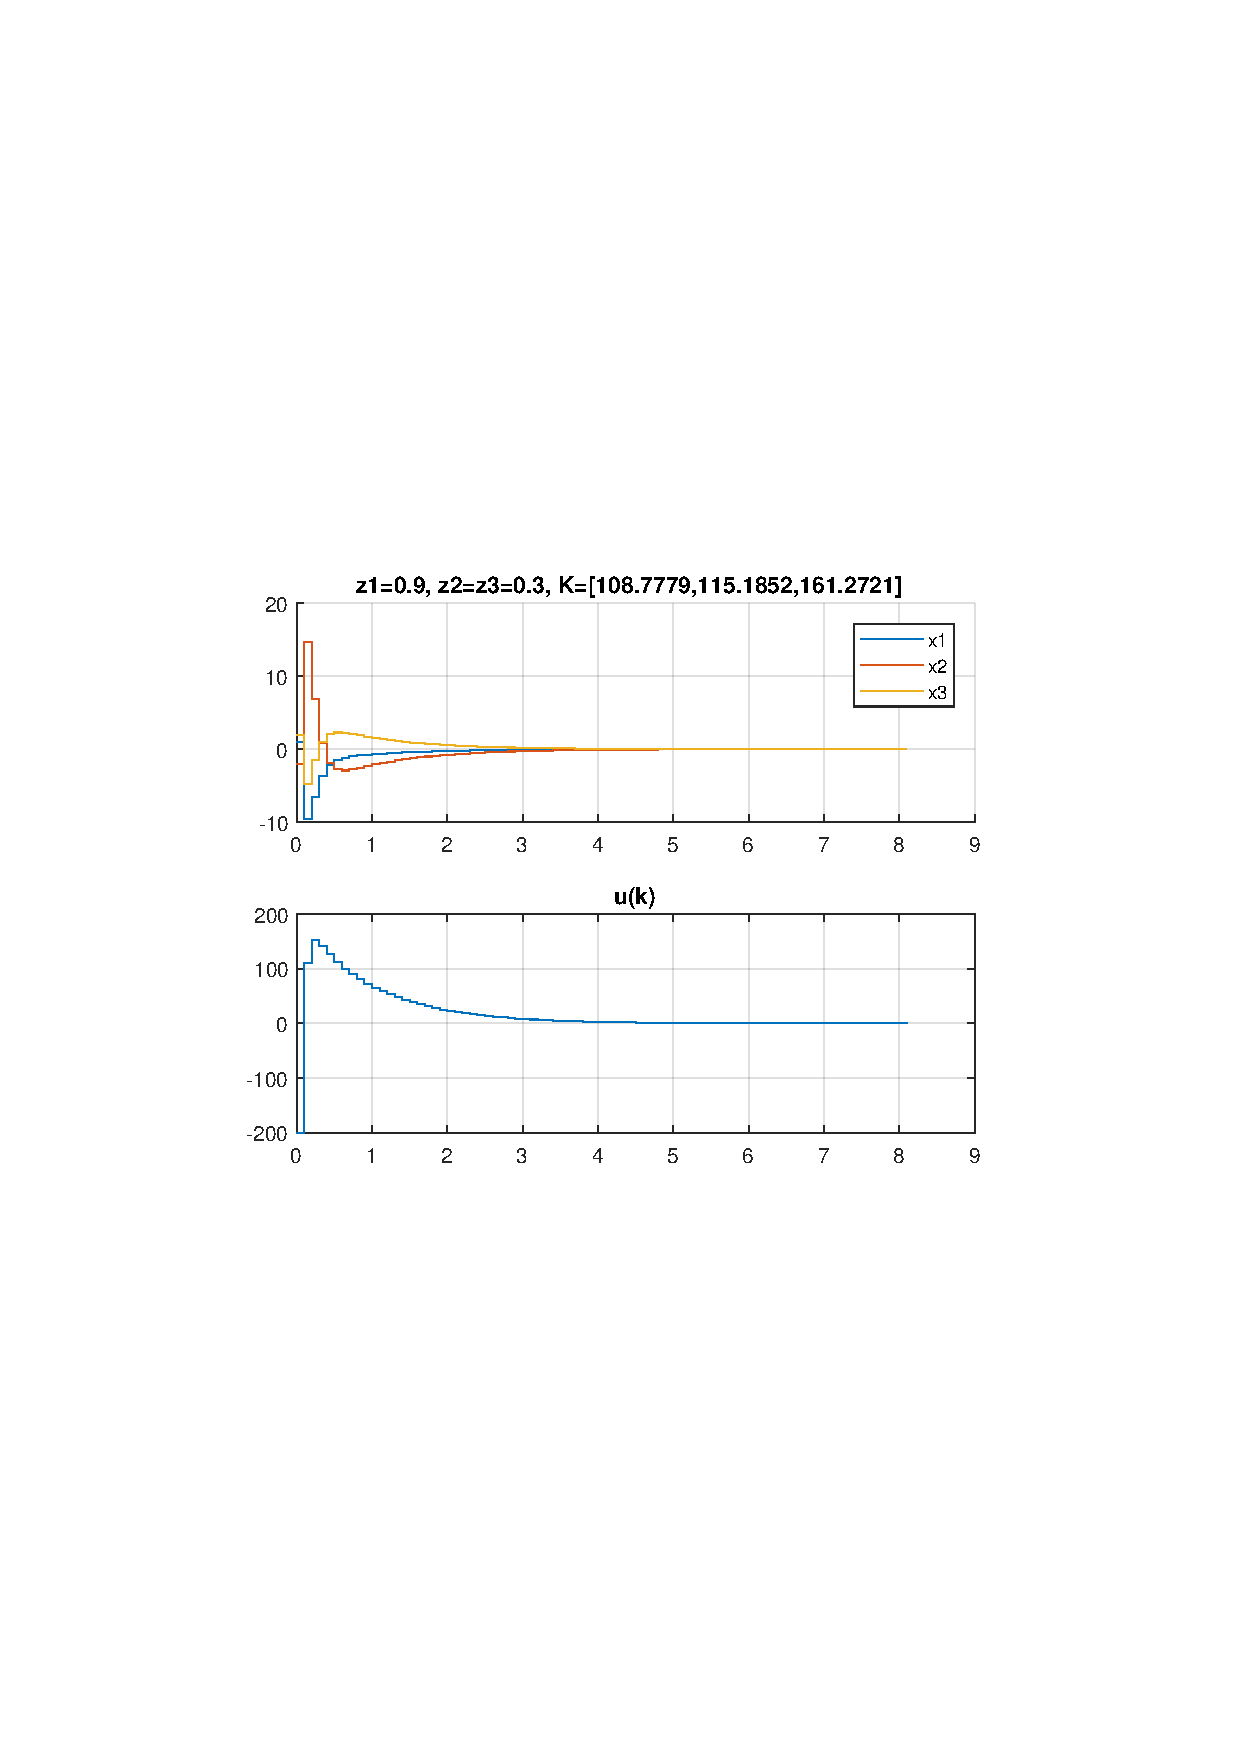
\includegraphics[clip, trim=0.5cm 9.5cm 0.5cm 9.5cm, width=1.00\textwidth]{../rys/zad3b_rys15.pdf}
\label{fig:rys3.2.15}
\caption{2.15}
\end{figure}

\begin{figure}[H]
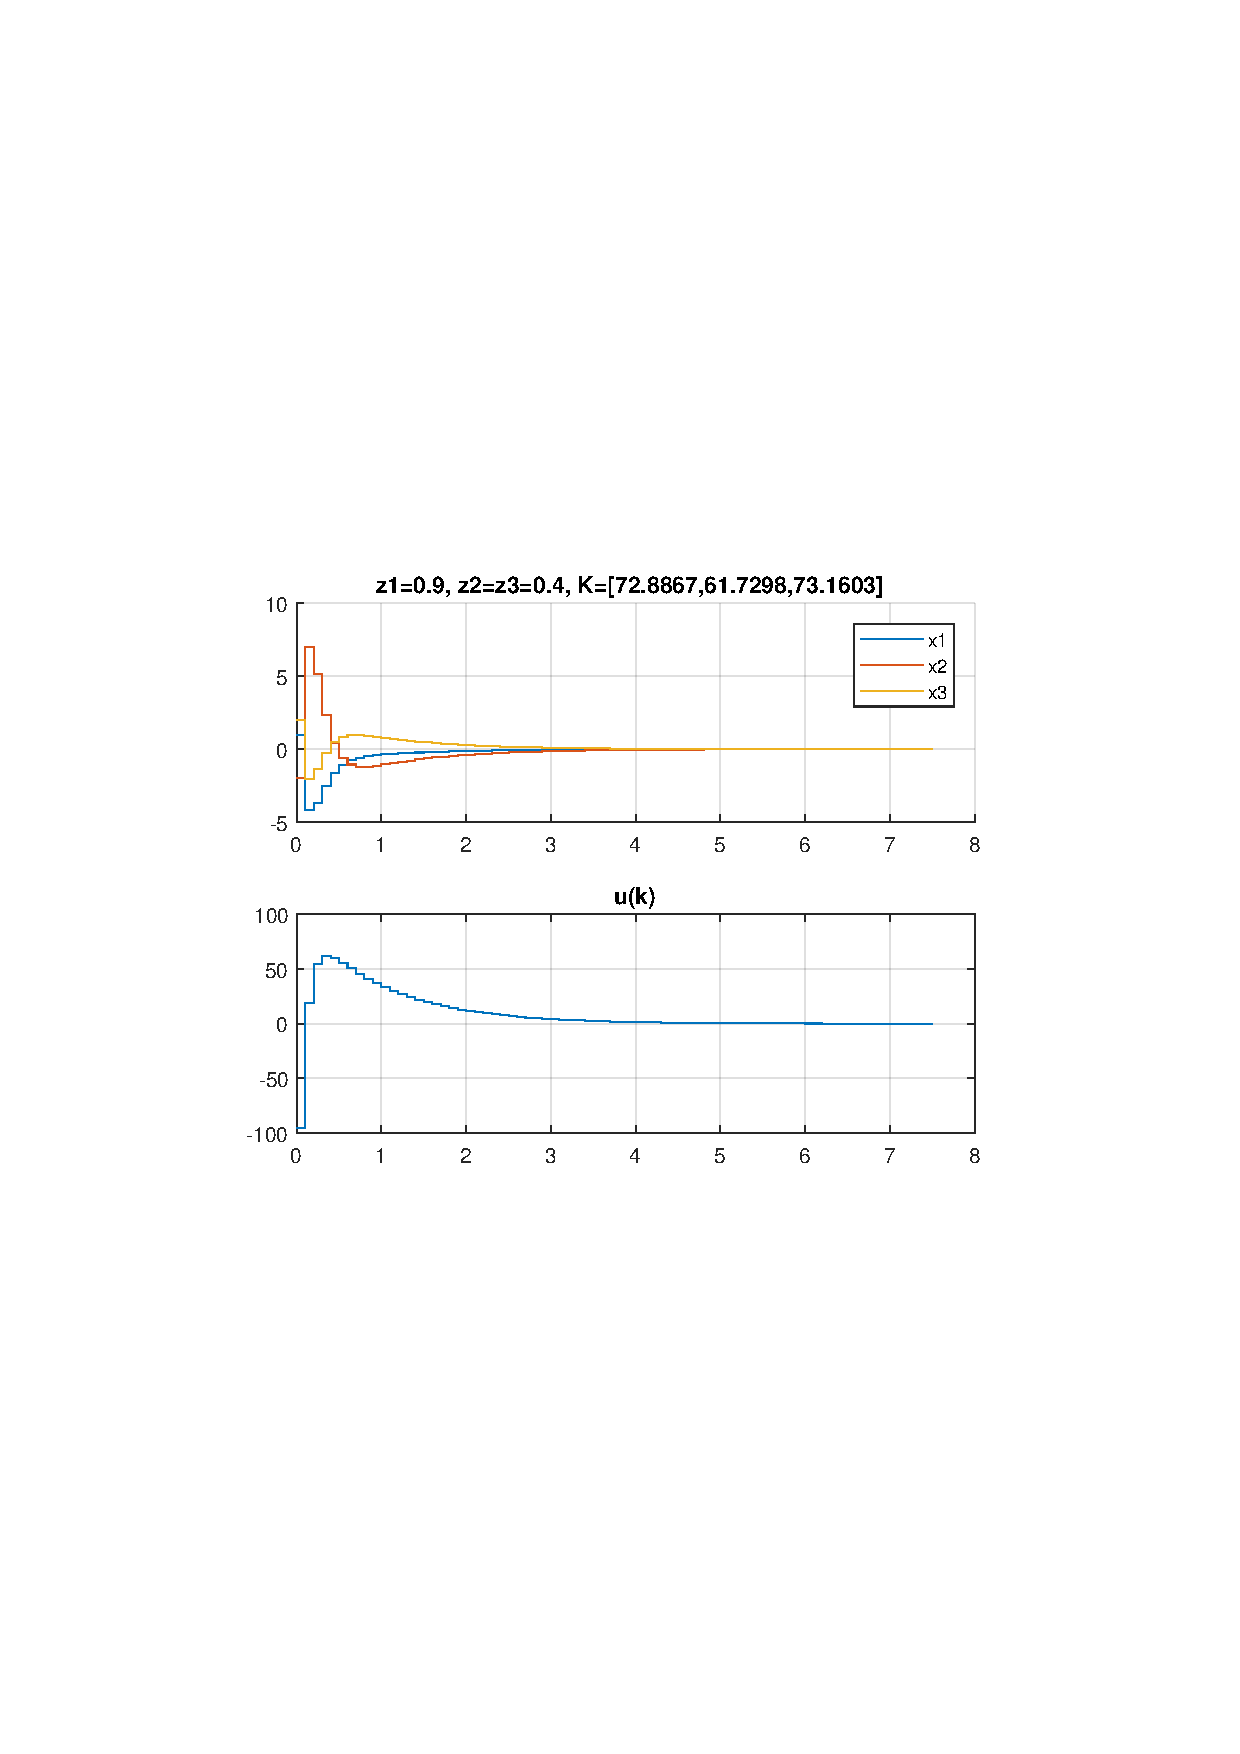
\includegraphics[clip, trim=0.5cm 9.5cm 0.5cm 9.5cm, width=1.00\textwidth]{../rys/zad3b_rys16.pdf}
\label{fig:rys3.2.16}
\caption{2.16}
\end{figure}
}
\vbox{
\subsubsection{Wnioski}
Układy o $z_1=0.6, z_2=z_3=0.3$ oraz $z_1=0.6, z_2=z_3=0.4$ stabilizują się szybko i mają małe przeregulowania. Tak dopasowany regulator dobrze spełnia swoje zadanie. Występują tu większe przeregulowania niż w wybranym układzie o jednakowych biegunach, jednak stabilizacja przebiega szybciej.
}
\subsection{Model}
\begin{figure}[H]
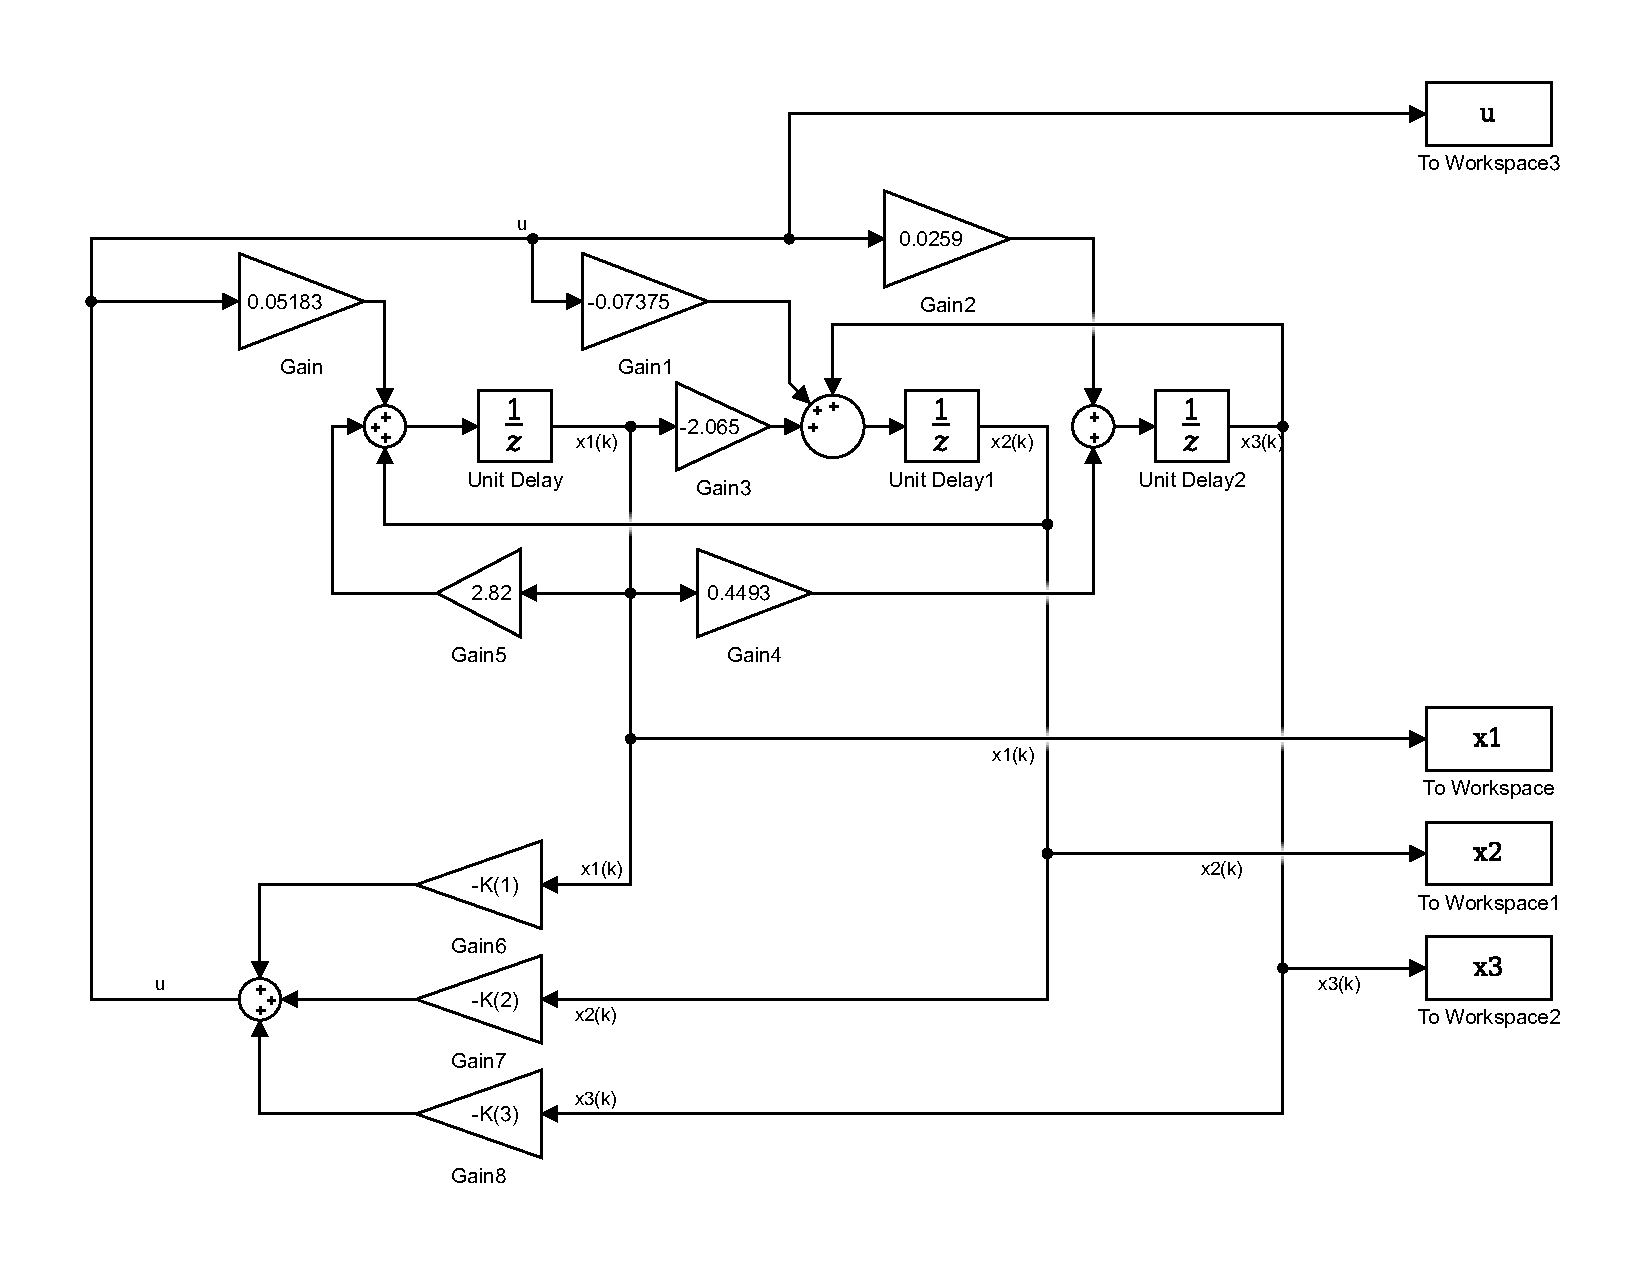
\includegraphics[clip, trim=0.5cm 0.5cm 0.5cm 0.5cm, width=1.00\textwidth]{../rys/zad3_model.pdf}
\label{fig:zad3mod}
\caption{Model układu zamkniętego}
\end{figure}
\newpage
\section{Zadanie 4}
\subsection{Treść}
Zaprojektować obserwator zredukowanego rzędu o biegunach $z_{o1}, z{_o2}$. Narysować strukturę
obserwatora i układu regulacji z obserwatorem. Do symulacji należy przyjąć zerowy stan 
początkowy dla obserwatora oraz niezerowy stan początkowy obiektu (jak wyżej).
Zastosować lepszy z dwóch regulatorów zaprojektowanych w punkcie 3. Położenie
biegunów obserwatora należy dobrać w taki sposób, aby obserwator był:\\
a) wolny,\\
b) szybki.\\
Należy zamieścić przebiegi zmiennych stanu i sterowania otrzymane podczas
eksperymentów dla obydwu przypadków.
\subsection{Obserwator zredukowanego rzędu}
\begin{figure}[H]
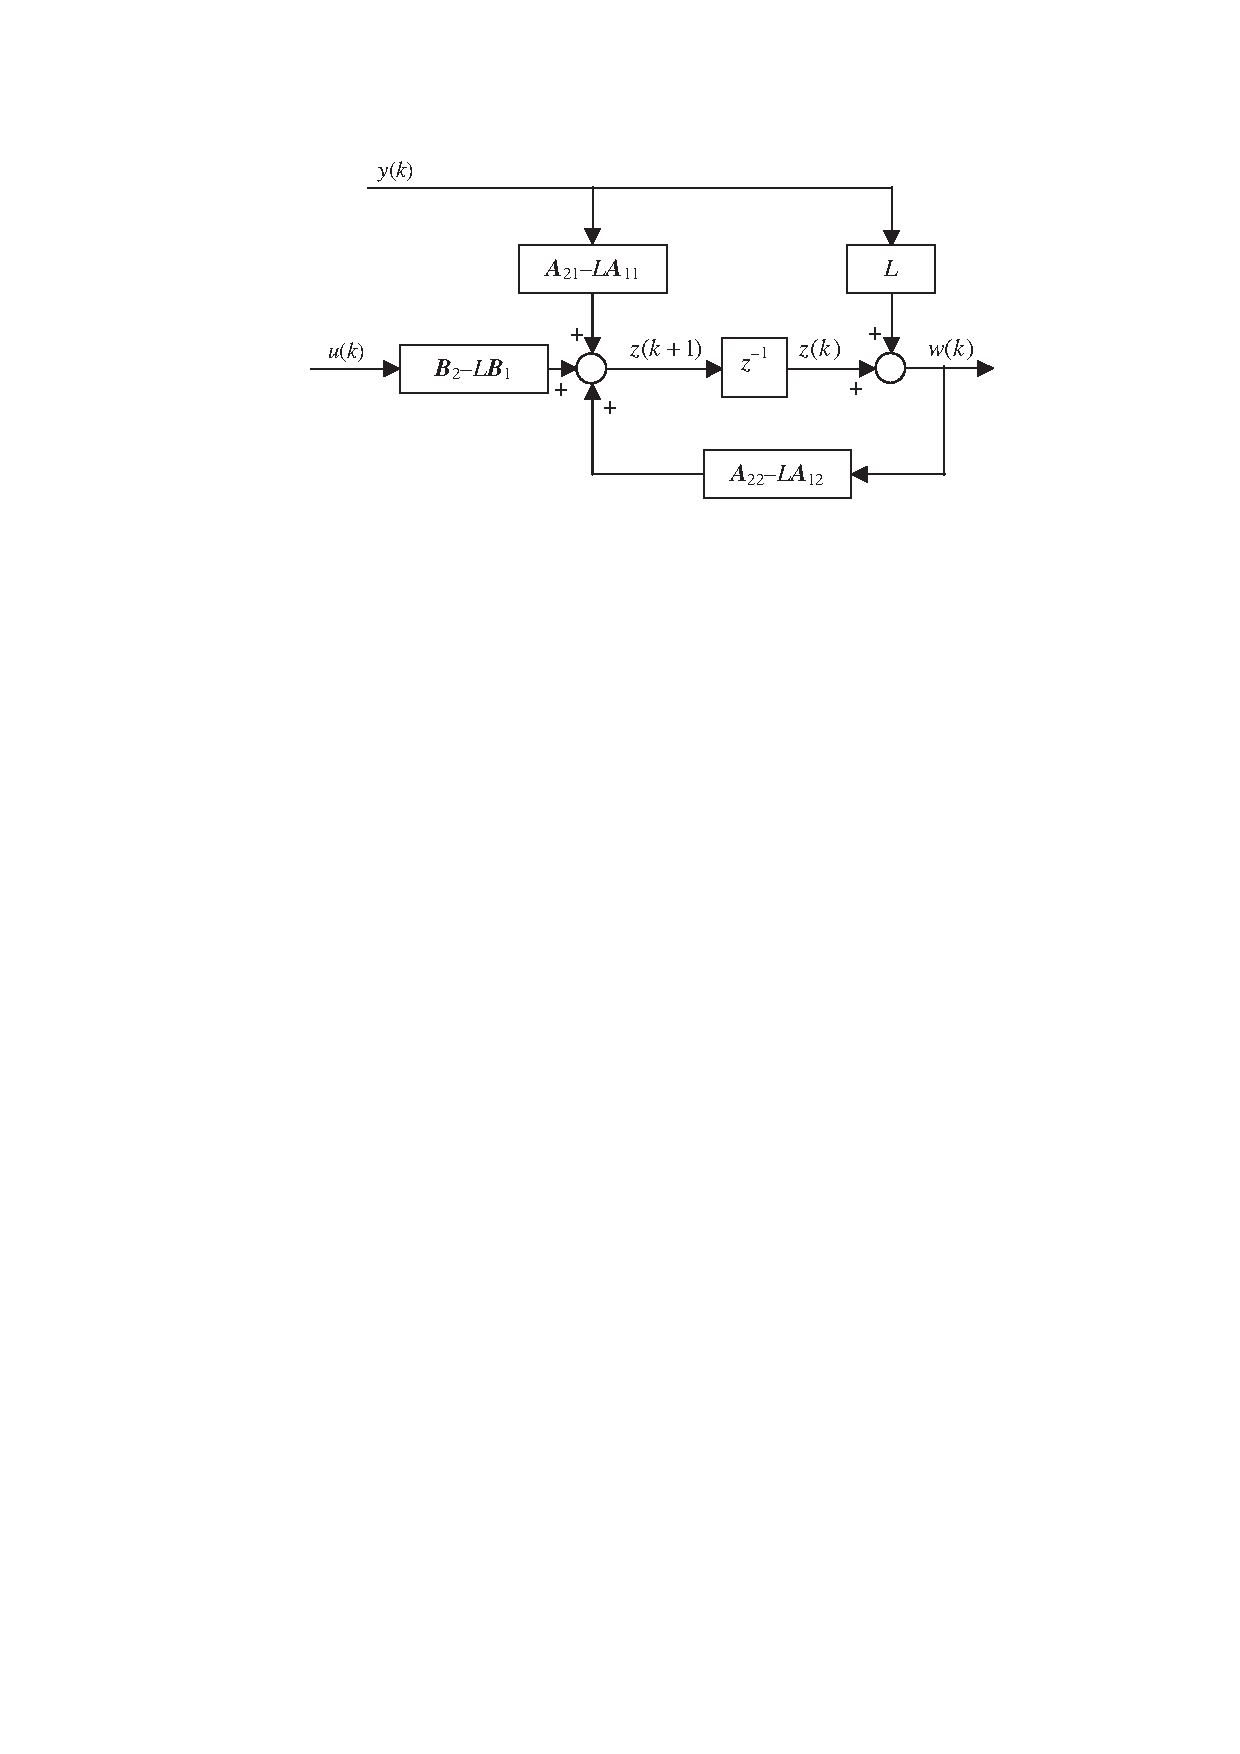
\includegraphics[clip, trim=0.5cm 0cm 0.5cm 0cm, width=1.00\textwidth]{../rys/obserwator.pdf}
\label{fig:zad4obs}
\caption{Struktura dyskretnego obserwatora zredukowanego rzędu}
\end{figure}
\vspace{0.5cm}

\subsection{Rozwiązanie}
\subsubsection{Wzór}
$$
x(k)=\left[\begin{array}{c} x_1(k)\\ w(k) \end{array}\right]=\left[\begin{array}{c} y(k)\\ w(k) \end{array}\right]
$$
$$
y(k)=x_1(k), w(k)=\left[\begin{array}{c} x_2(k)\\ x_3(k) \end{array}\right]
$$
$$
z(k)=w(k)-Ly(k)
$$
$$
z(k+1)=(A_{22}-LA_{12})(z(k)+Ly(k))+(A_{21}-LA{11})y(k)+(B_2-LB_1)u(k)
$$

Przyjmuję oznaczenia:
$$
A=\left[\begin{array}{ccc} a_{1} & 1 & 0\\ a_{2} & 0 & 1\\ a_{3} & 0 & 0 \end{array}\right]
$$

$$
B=\left[\begin{array}{c} b_{1}\\ b_{2}\\ b_{3} \end{array}\right], L=\left[\begin{array}{c} l_{1}\\ l_{2} \end{array}\right]
$$

Na podstawie powyższych wzorów przy pomocy matlaba wyznaczyłem następujące równania:

$$
z(k)=\left[\begin{array}{c} x_{2}-l_{1}\,x_{1}\\ x_{3}-l_{2}\,x_{1} \end{array}\right]
$$
$$
z(k+1)=\left[\begin{array}{c} x_{3}-l_{1}\,x_{2}+u\,\left(b_{2}-b_{1}\,l_{1}\right)+x_{1}\,\left(a_{2}-a_{1}\,l_{1}\right)\\ u\,\left(b_{3}-b_{1}\,l_{2}\right)-l_{2}\,x_{2}+x_{1}\,\left(a_{3}-a_{1}\,l_{2}\right) \end{array}\right]
$$

\subsubsection{Model obserwatora}
\begin{figure}[H]
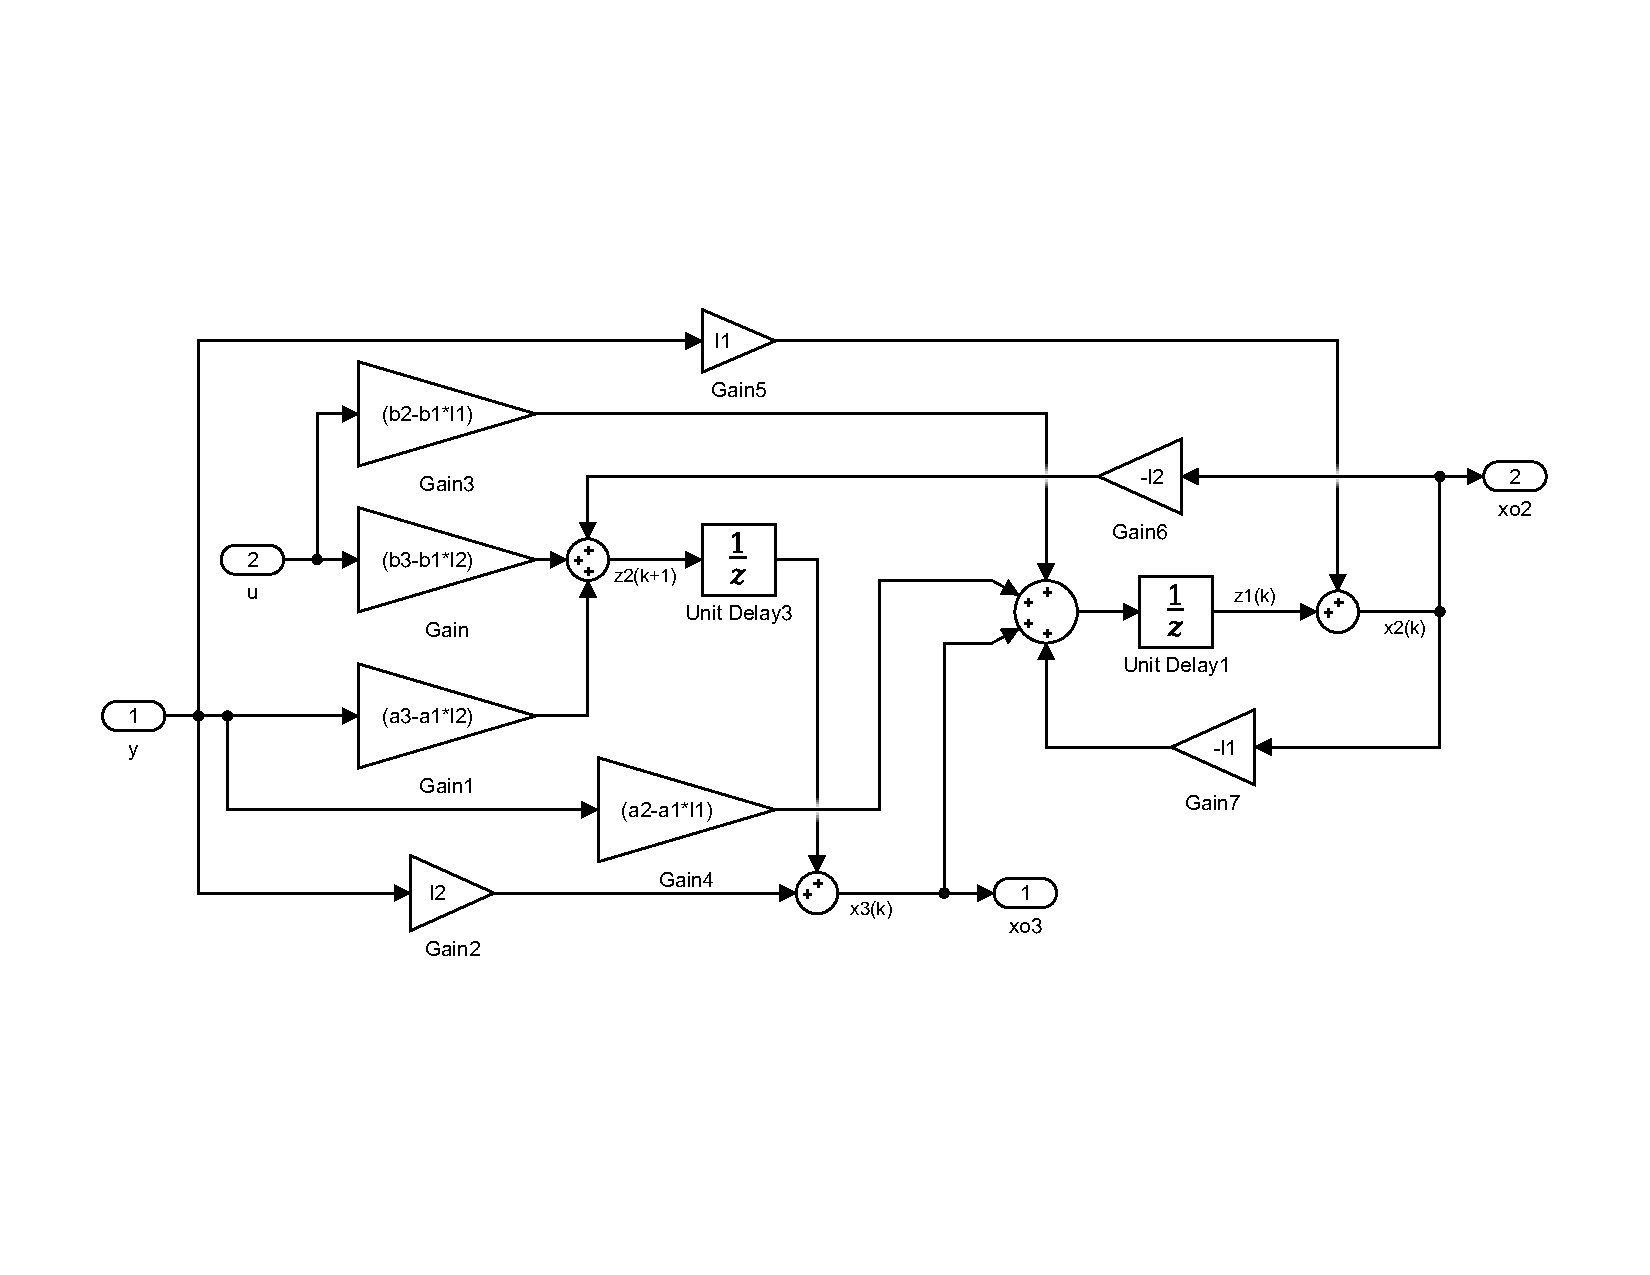
\includegraphics[clip, trim=0cm 4cm 0cm 4cm, width=1.00\textwidth]{../rys/zad4_obserwator.pdf}
\label{fig:zad4obs}
\caption{Zrealizowany obserwator}
\end{figure}
\newpage
\subsubsection{Struktura układu regulacji z obserwatorem}
\begin{figure}[H]
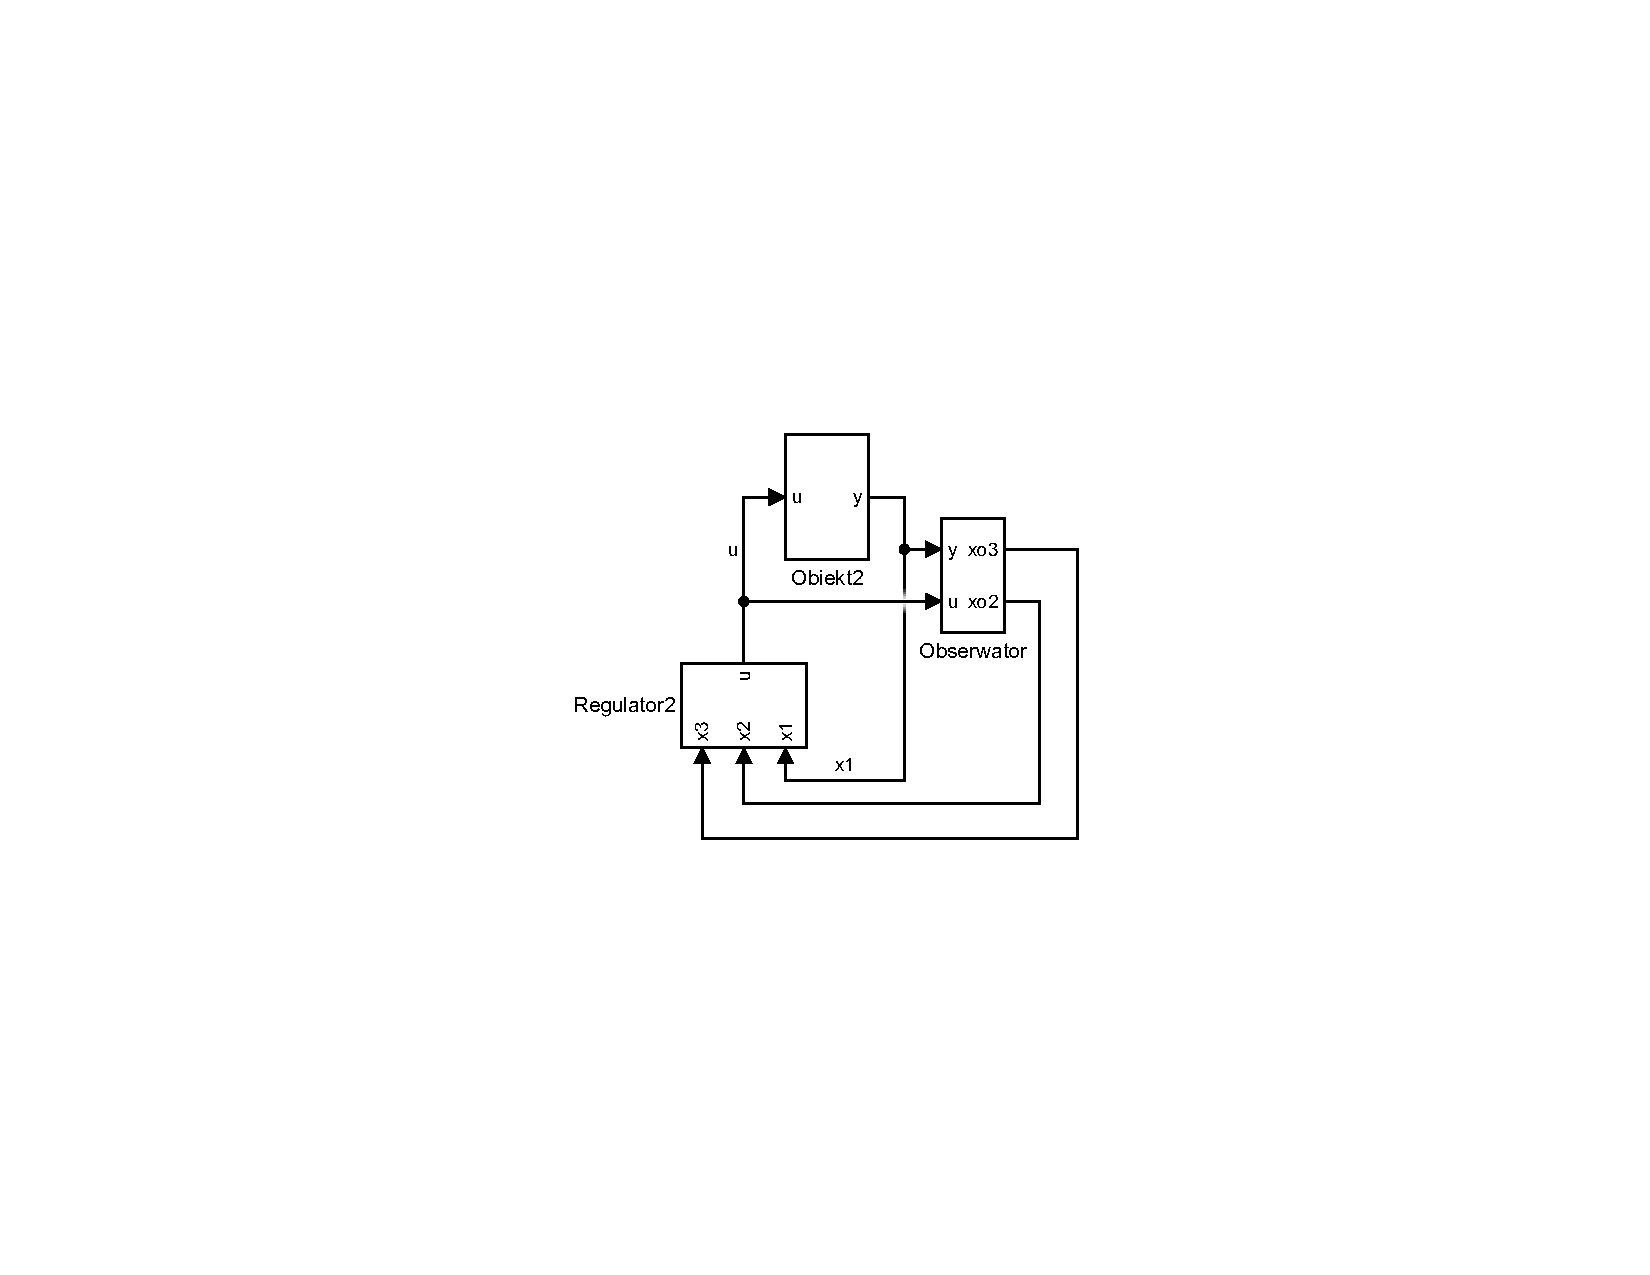
\includegraphics[clip, trim=9cm 7cm 9cm 7cm, width=1.00\textwidth]{../rys/zad4_regobs.pdf}
\label{fig:zad4regobs}
\caption{Struktura układu}
\end{figure}
\subsubsection{Wykresy}
\begin{figure}[H]
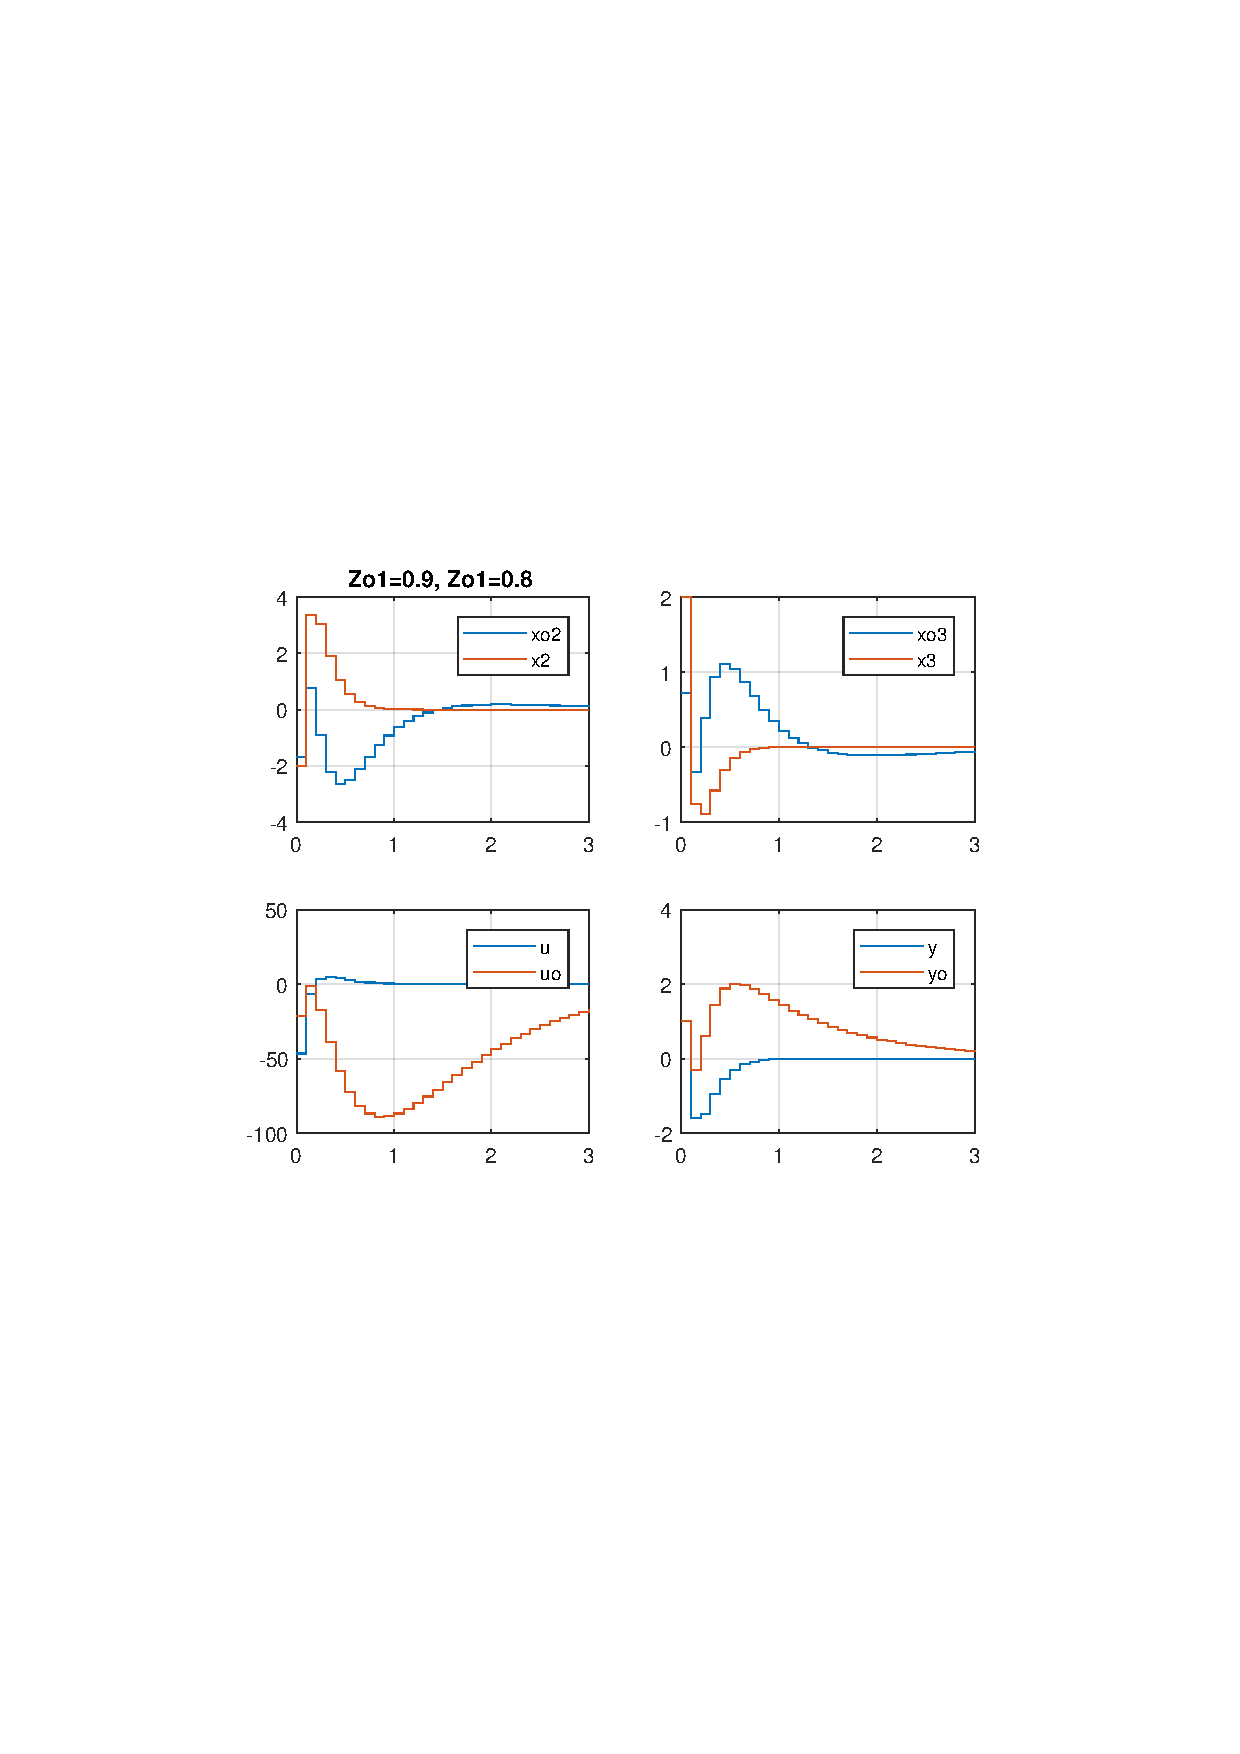
\includegraphics[clip, trim=2cm 10cm 2cm 9.5cm, width=1.00\textwidth]{../rys/zad4_rys1.pdf}
\label{fig:rys4.1}
\caption{4.1}
\end{figure}

\begin{figure}[H]
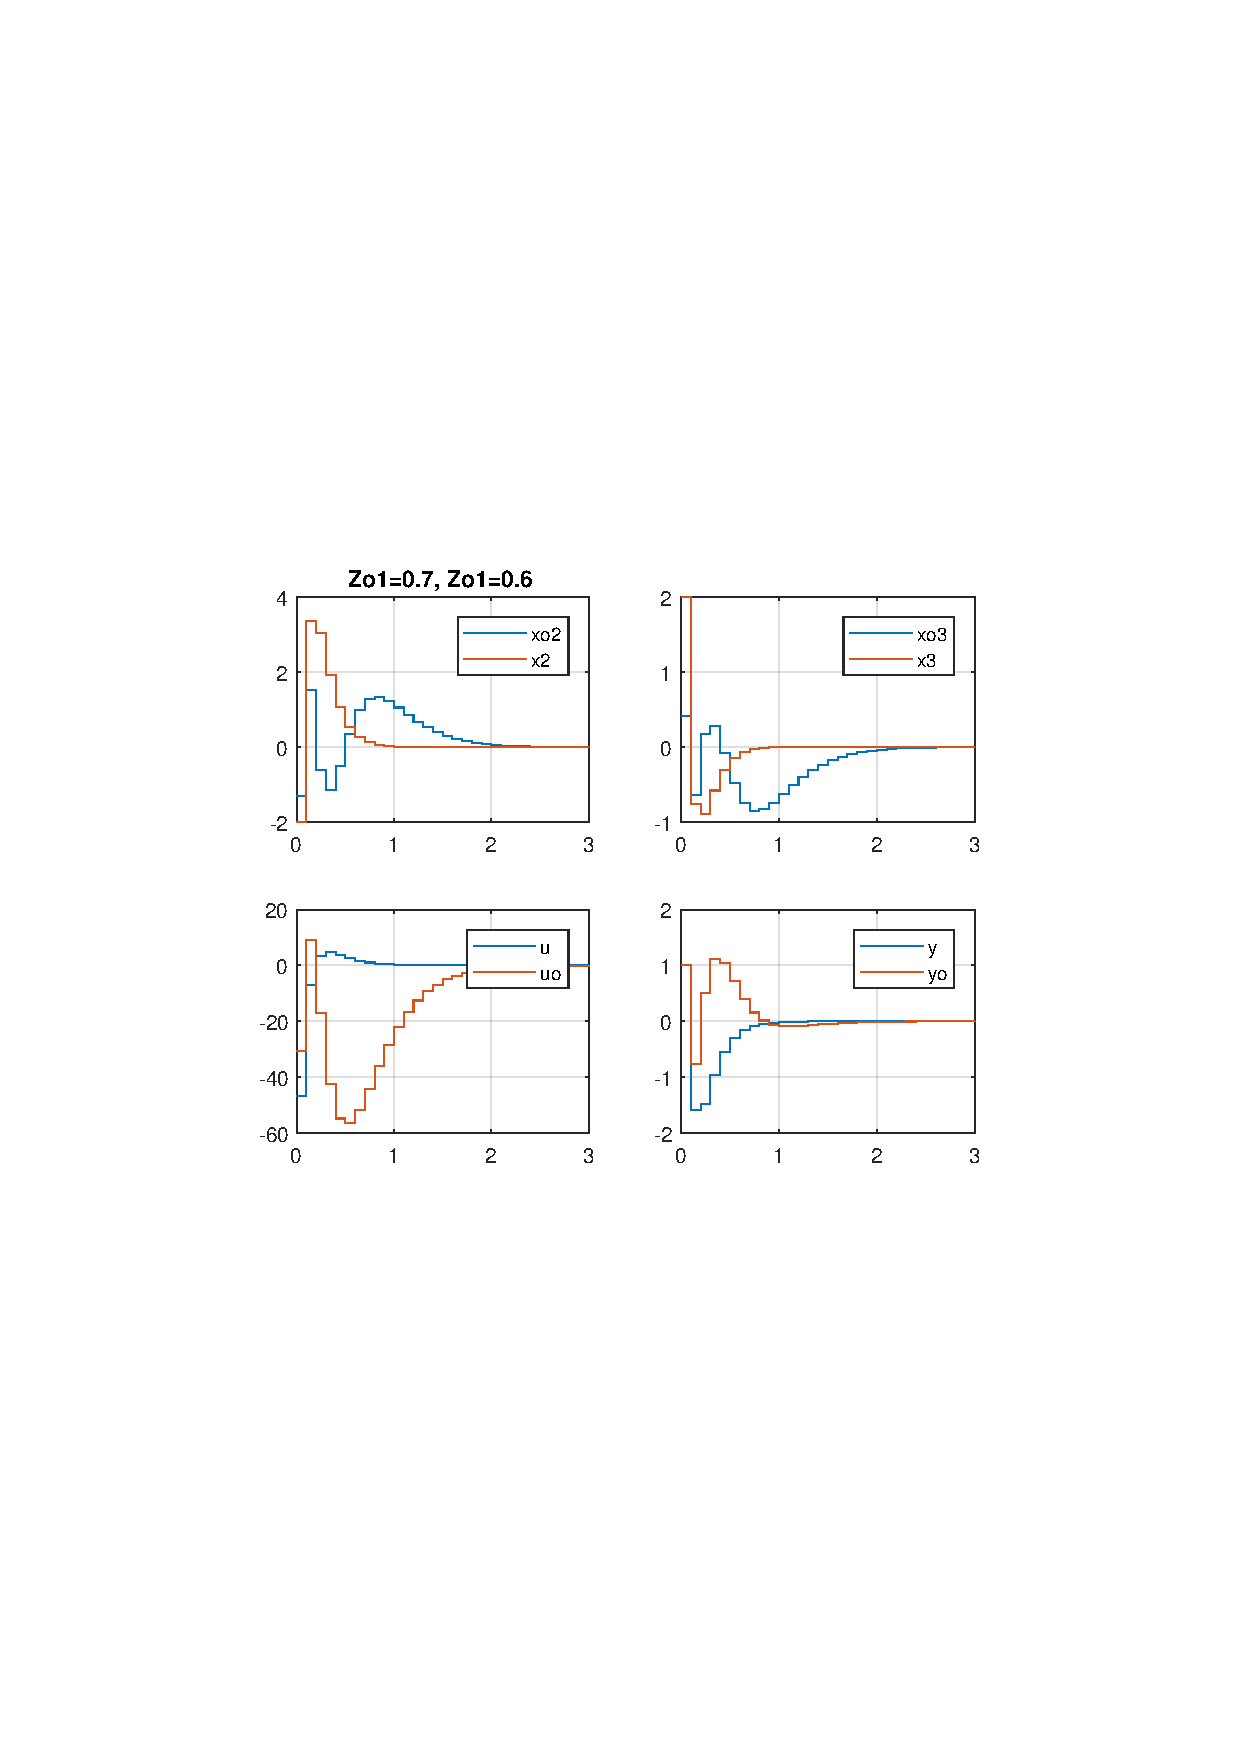
\includegraphics[clip, trim=2cm 10cm 2cm 9.5cm, width=1.00\textwidth]{../rys/zad4_rys2.pdf}
\label{fig:rys4.2}
\caption{4.2}
\end{figure}

\begin{figure}[H]
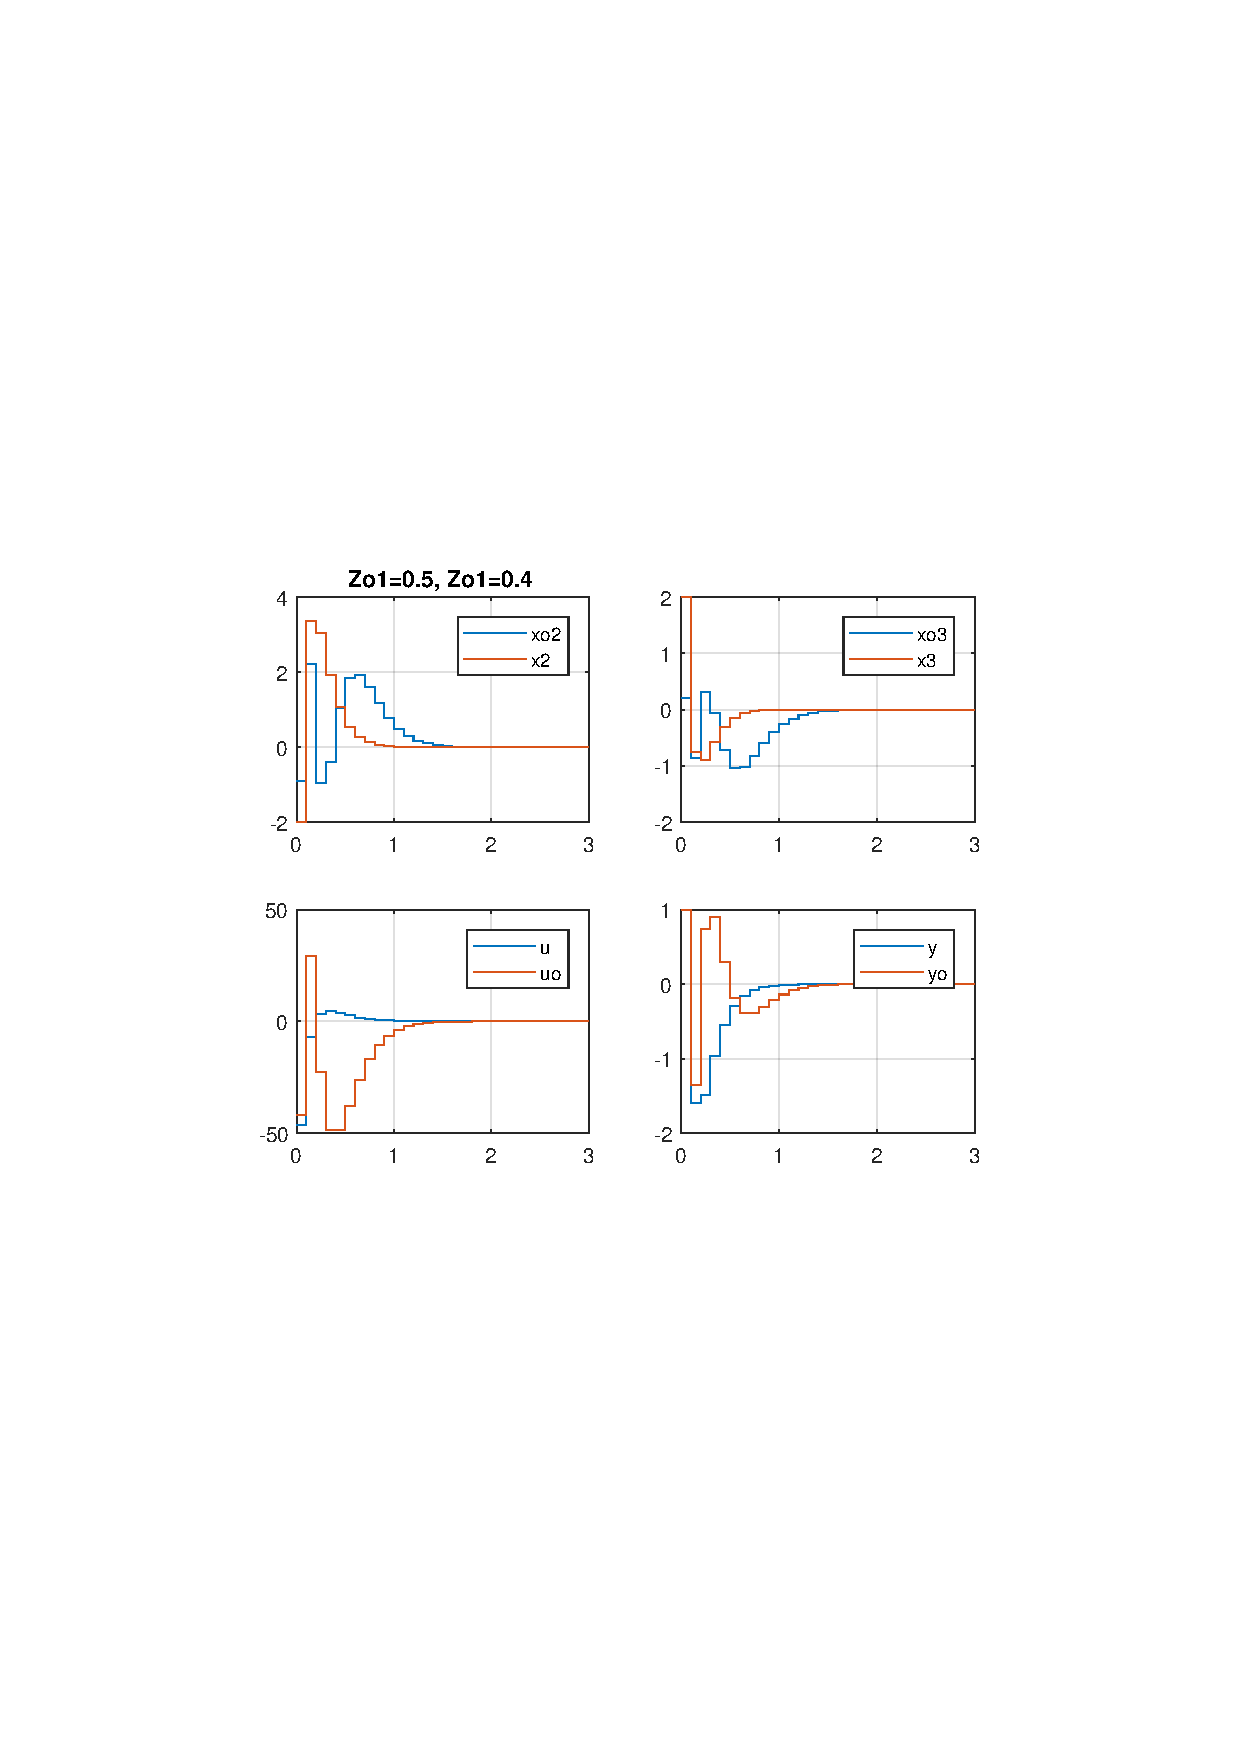
\includegraphics[clip, trim=2cm 10cm 2cm 9.5cm, width=1.00\textwidth]{../rys/zad4_rys3.pdf}
\label{fig:rys4.3}
\caption{4.3}
\end{figure}

\begin{figure}[H]
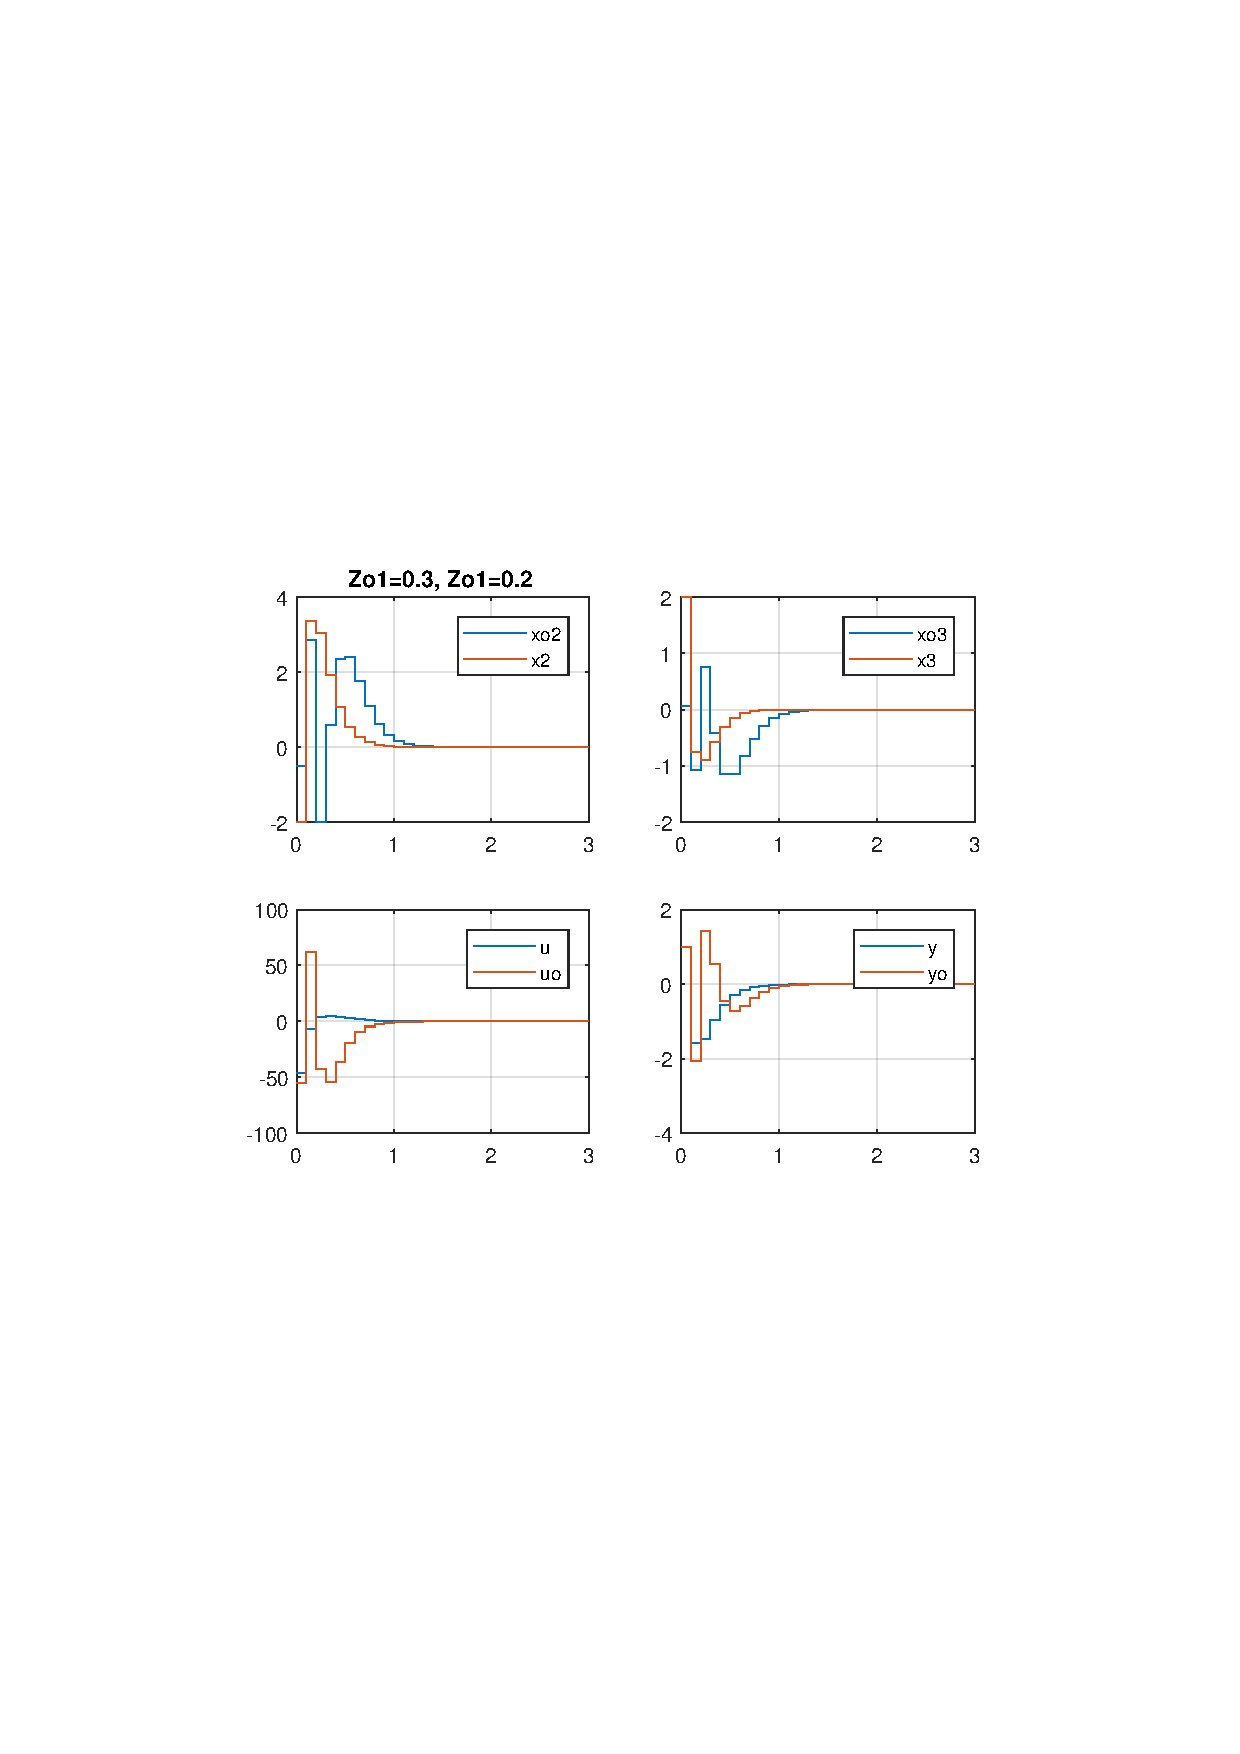
\includegraphics[clip, trim=2cm 10cm 2cm 9.5cm, width=1.00\textwidth]{../rys/zad4_rys4.pdf}
\label{fig:rys4.4}
\caption{4.4}
\end{figure}

\begin{figure}[H]
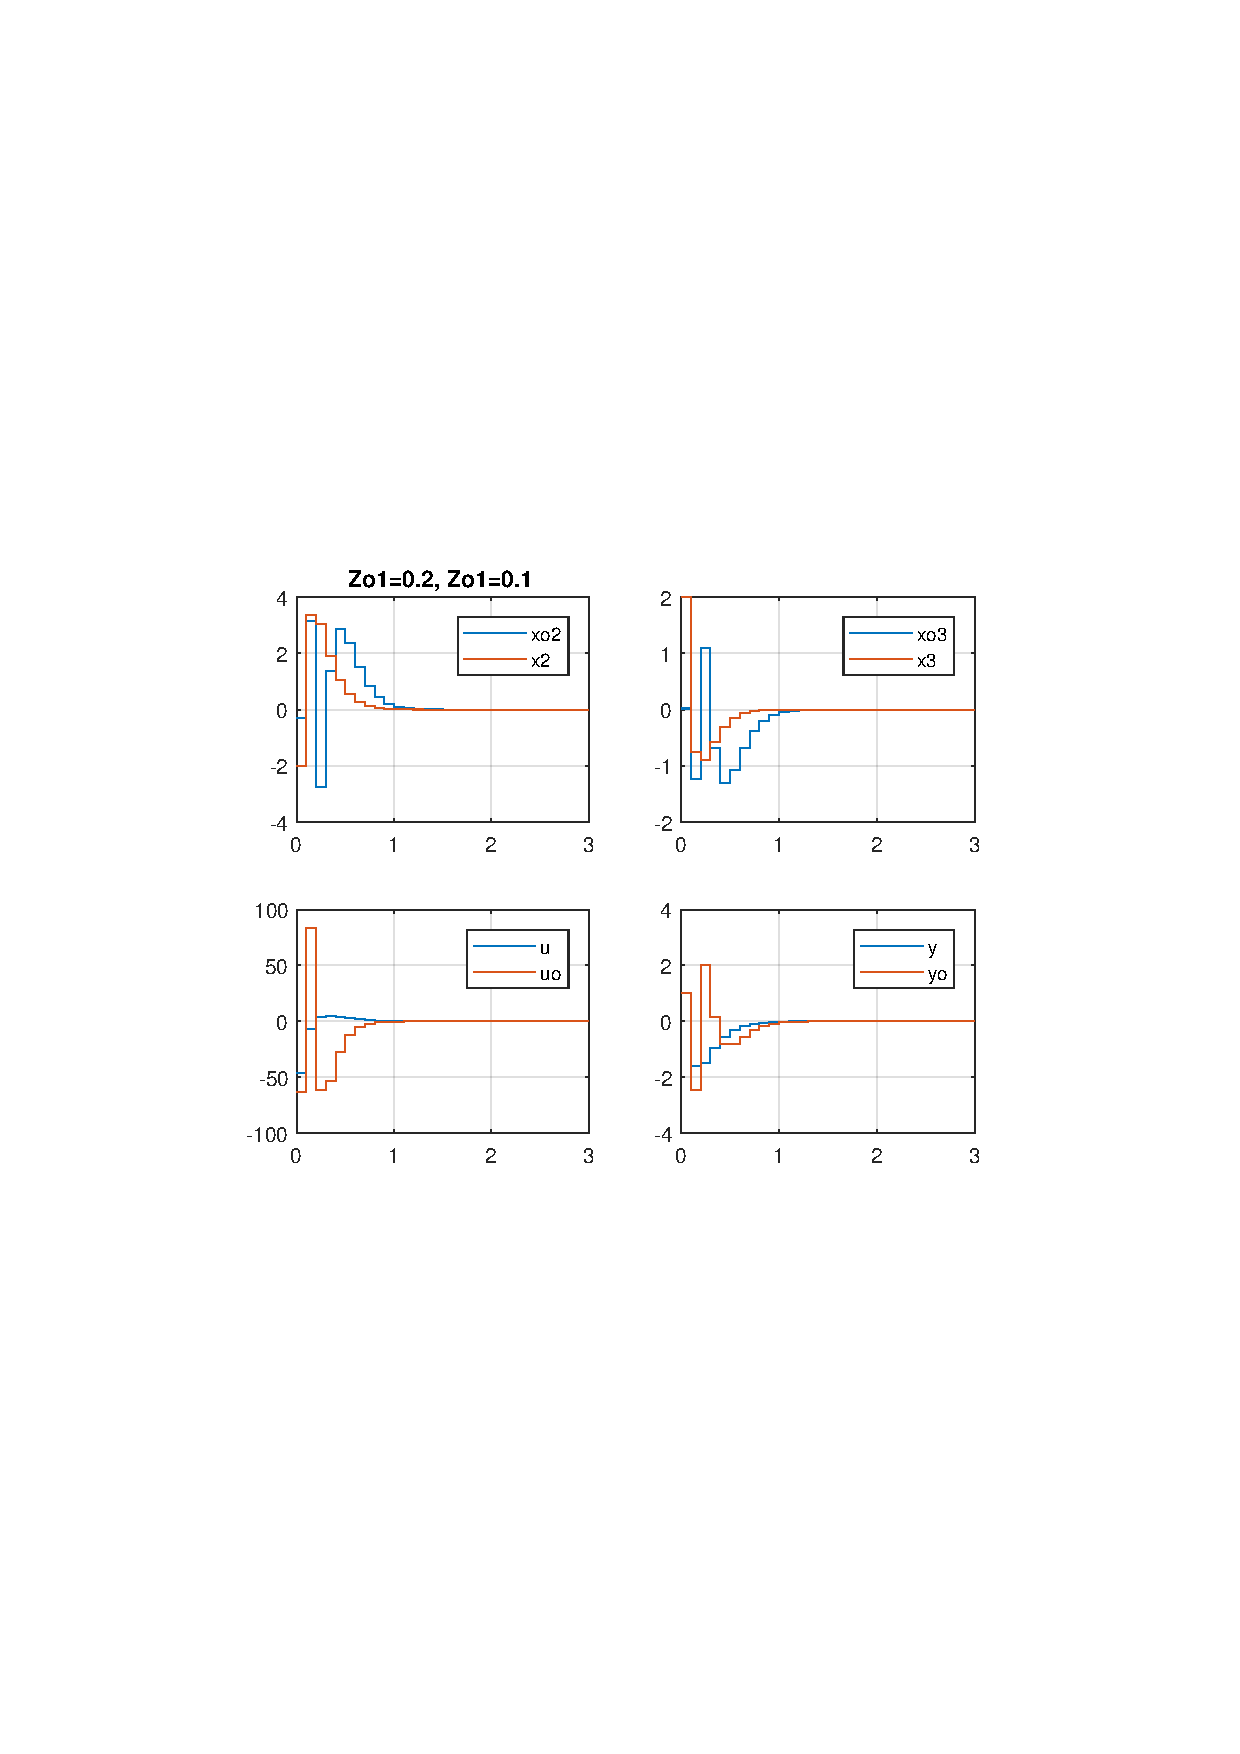
\includegraphics[clip, trim=2cm 10cm 2cm 9.5cm, width=1.00\textwidth]{../rys/zad4_rys5.pdf}
\label{fig:rys4.5}
\caption{4.5}
\end{figure}
\subsubsection{Wnioski}
Z otrzymanych wykresów wynika, że przy doborze obserwatora należy tak dobrać bieguny, aby osiągnąć kompromis pomiędzy szybkością działania, a brakiem przeregulowań. Szybszy obserwator, czyli ten o biegunach bliższych zera, ma większe przeregulowania niż wolny.
Zatem wybór położenia biegunów jest uwarunkowany tym co jest ważniejsze w danym projekcie.

\end{document}